\documentclass[utf8, diplomski, lmodern]{fer}

% font
\renewcommand{\familydefault}{\sfdefault}  % sans-serif main

%\usepackage[cm]{sfmath}  % bolje nego mathastext
%\SetSymbolFont{largesymbols}{normal}{OMX}{iwona}{m}{n}

%\usepackage[italic]{mathastext}  % sfmath je bolje (manji indeksi)


%\usepackage{inconsolata}					% sans-serif monospace
\usepackage[scaled]{beramono}				% sans-serif monospace


%\usepackage[math]{iwona}
%\usepackage[math]{kurier}

%\newcommand*{\scale}[2][4]{\scalebox{#1}{$#2$}} % \Scale[0.5]{y = \sin^2 x}
%\usepackage{scalerel}


\usepackage[T1]{fontenc}  % accented characters, copy from pdf, ...

\raggedright						% bez desnog poravnavanja

\usepackage{caption}
\captionsetup{%
	justification=raggedright,
}
\usepackage{etoolbox}
\makeatletter
	\patchcmd{\@dottedtocline}
	{\rightskip\@tocrmarg}
	{\rightskip\@tocrmarg plus 4em \hyphenpenalty\@M}
	{}{}
\makeatother
\setlength{\parindent}{1em}	 % uvlačenje ulomaka
\usepackage{indentfirst}	 % uvlačenje prvog ulomka
\setlength{\parskip}{0.5em}	 % razmak između ulomaka

\usepackage{listings}  % listings
\renewcommand{\lstlistingname}{Ispis}

\usepackage[multiple]{footmisc}	 % višestruke fusnote

\usepackage[hidelinks]{hyperref}
\renewcommand*{\UrlFont}{\footnotesize}

% colors

\usepackage{xcolor}
\usepackage{color}

\hypersetup{
	colorlinks,
	linkcolor={blue!60!green!50!black},  % xcolor package
	citecolor={green!40!black},
	urlcolor={blue!75!green!30!black}
}
\definecolor{bluekeywords}{rgb}{0.13,0.13,1}  % color package
\definecolor{greencomments}{rgb}{0,0.5,0}
\definecolor{redstrings}{rgb}{0.9,0,0}

\DeclareTextFontCommand{\emphasize}{\bfseries}

\newtheorem{theorem}{Teorem}[section]
\newtheorem{definition}{Definicija}[section]

\usepackage{enumitem}  % \begin{enumerate}[topsep=0pt,itemsep=0pt,partopsep=0pt]

% redefinition of left and right to make spacing consistent
\let\originalleft\left
\let\originalright\right
\def\left#1{\mathopen{}\originalleft#1}
\def\right#1{\originalright#1\mathclose{}}

\usepackage{amsmath}
\usepackage{mathtools}  % \coloneqq
%\usepackage{bm}
%\usepackage[utopia]{mathdesign}
\usepackage[OMLmathsfit]{isomath}  % \DeclareMathAlphabet ...

\usepackage{mathtools}  % smashoperator
\usepackage{commath}  % calculus, perentheses
\usepackage{stmaryrd}  % \llbracket for \rrbracket, ...


%\usepackage[croatian]{babel}		% teorem
%\newtheorem{definition}{Definicija}[section]
%\newtheorem{theorem}{Teorem}[section]
%\newtheorem{corollary}{Korolar}[theorem]

\DeclareMathAlphabet{\mathbbmsl}{U}{bbm}{m}{sl}
\DeclareMathAlphabet{\mathbbmb}{U}{bbm}{b}{it}
\DeclareMathAlphabet{\mathbbmssit}{U}{bbmss}{m}{it}


% common set?, distribution
\newcommand{\commset}[1]{\mathbbmb{#1}}
\newcommand{\distrib}[1]{\mathcal{#1}}

% sans-serif blackboard-bold
\newcommand{\mathsfbbit}[1]{\mathbbmssit{#1}}

% variable
\let\vec\relax
\let\set\relax
\newcommand{\vec}[1]{\mathbfit{#1}}
\newcommand{\mat}[1]{\vec{#1}}
\newcommand{\ten}[1]{\vec{#1}}
\newcommand{\set}[1]{\mathbbmsl{#1}}

% constant
\newcommand{\const}[1]{\mathrm{#1}}
\newcommand{\cvec}[1]{\mathbf{#1}}
\newcommand{\cmat}[1]{\cvec{#1}}
\newcommand{\cten}[1]{\cvec{#1}}
\newcommand{\cset}[1]{\mathbb{#1}}

% random variable
\newcommand{\rvar}[1]{{\color{green!50!blue!40!black}\mathsfit{#1}}}
\newcommand{\rvec}[1]{{\color{green!50!blue!40!black}\mathsfbfit{#1}}}
\newcommand{\rmat}[1]{\rvec{#1}}
\newcommand{\rten}[1]{\rvec{#1}}
\newcommand{\rset}[1]{{\color{green!50!blue!40!black}\mathsfbbit{#1}}}

% linear algebra
\newcommand{\transpose}{\mathsf T}

% calculus - commath: od, pd, md, dif
% parentheses - commath: del, cbr, sbr, envert, enVert

% named functions
\DeclareMathOperator{\softplus}{softplus}
\DeclareMathOperator{\softmax}{softmax}
\DeclareMathOperator{\logistic}{\sigma}
\DeclareMathOperator{\sgn}{sgn}
\DeclareMathOperator{\diag}{diag}

% operators
\DeclareMathOperator*{\argmin}{arg\,min} % thin space
\DeclareMathOperator*{\argmax}{arg\,max}
\let\P\relax
\DeclareMathOperator*{\P}{\mathrm{P}}
\DeclareMathOperator*{\p}{\mathrm{p}}
\DeclareMathOperator*{\E}{\mathrm{I\kern-.282em E}}
\DeclareMathOperator*{\D}{\mathrm{I\kern-.282em D}}
\DeclareMathOperator*{\Cov}{\mathrm{Cov}}
%\let\H\relax
\renewcommand{\H}{\mathrm{H}}
\newcommand{\I}{\mathrm{I}}
\DeclareMathOperator*{\Dklsym}{D_{\mathrm{KL}}}

% bracket operators
\newcommand{\enangle}[1]{\mathinner{\left\langle{#1}\right\rangle}}
\newcommand{\enbbracket}[1]{\mathinner{\left\llbracket{#1}\right\rrbracket}}
\newcommand{\braket}[2]{\enangle{{#1}|{#2}}}

% parentheses from commath redefined to improve spacing because (left and right were redefined)
\renewcommand{\del}[1]{\left(#1\right)}
\renewcommand{\sbr}[1]{\left[#1\right]}
\renewcommand{\cbr}[1]{\left\{#1\right\}}
\renewcommand{\intoo}[1]{\mathinner{\del{#1}}}
\renewcommand{\intcc}[1]{\mathinner{\sbr{#1}}}
\renewcommand{\intco}[1]{\mathinner{\left[#1\right)}}
\renewcommand{\intoc}[1]{\mathinner{\left(#1\right]}}

% special
\newcommand{\funcdef}[3]{#1 \colon #2 \to #3}
\newcommand{\Dkl}[2]{\Dklsym\del{#1\;\middle\|\;#2}}
\newcommand{\C}{\cset{C}}
\newcommand{\R}{\cset{R}}
\newcommand{\Z}{\cset{Z}}
\newcommand{\N}{\cset{N}}
\newcommand{\dirac}{\delta}
\newcommand{\ind}[2]{#1_{\sbr{#2}}}

% operators
\newcommand{\bidot}{\mkern1.5mu{..}\mkern1.5mu}
\newcommand\sheq{\mkern1.5mu{=}\mkern1.5mu}
%\renewcommand{\dots}{...}
\usepackage{booktabs}  % from the tamplate; table quality enhancement

\usepackage{multirow}
\usepackage{tabularx}

%\usepackage{floatrow} 				% centriranje svih slika
\usepackage{float}					% figure [H]
\usepackage{graphicx} 				% includegraphics
\usepackage{caption}			% subfigure
\usepackage{subcaption}			% subfigure
\usepackage[export]{adjustbox} 	% http://ctan.org/pkg/adjustbox

\usepackage[section]{placeins}  % [section] for \FloatBarrier before every section 

\graphicspath{ {./figures/} }		% mapa sa slikama
%\let\oldincludegraphics\includegraphics
%\renewcommand{\includegraphics}[2][]{\oldincludegraphics[#1,max width=0.9\linewidth]{#2}}

%\usepackage{flafter} % floats after the first reference

\usepackage{tikz} 					% dijagrami
\usepackage{pgfplots}
\usetikzlibrary{fit,automata,arrows,positioning,calc,petri,topaths,arrows.meta}
	
\pgfplotsset{every axis/.append style={
		axis x line=middle,    	% put the x axis in the middle
		axis y line=middle,    	% put the y axis in the middle
		axis line style={->},  	% arrows on the axis
		xlabel={$x$},          	% default put x on x-axis
		ylabel={$y$},          	% default put y on y-axis
		samples=100,
		axis equal,
}} % axis style

\tikzset{
	>={Triangle[length=2mm,width=1.4mm]},
	dedge/.style={arrows=->, black, thick},
}
% PGMs
\tikzstyle{textnode} = [minimum size=5mm, node distance=9mm]
\tikzstyle{pnode} = [circle, minimum size=10mm, thick, draw=black, node distance=9mm]
\tikzstyle{greypnode} = [pnode, fill=black!5]
% https://github.com/jluttine/tikz-bayesnet
\tikzstyle{wrap} = [inner sep=0pt, fit=#1]
\tikzstyle{plate} = [draw, rectangle, rounded corners=0.5ex, thick, fit=#1]
\tikzstyle{caption} = [font=\footnotesize, node distance=0]
\tikzstyle{plate caption} = [caption, node distance=0, inner sep=0pt,
below left=5pt and 0pt of #1.south east]
\newcommand{\plate}[4][]{
	\node[wrap=#3] (#2-wrap) {};
	\node[plate caption=#2-wrap] (#2-caption) {#4};
	\node[plate=(#2-wrap)(#2-caption), #1] (#2) {};
}
% ANNs
\tikzstyle{nnode} = [circle, minimum size=10mm, thick, draw=black, node distance=5mm]
\tikzstyle{nrect} = [rectangle, minimum size=5mm, thick, draw=black, node distance=5mm, rounded corners=0.1ex]
\usepackage{dirtree}

\usepackage[]{algorithmic}

\usepackage{setspace}  % line spacing

%\usepackage{pythontex}


\usepackage[symbols,nopostdot,nonumberlist,section]{glossaries-extra}

%\renewcommand{\glossarypreamble}{\footnotesize}

\newglossarystyle{supergroup}{%
	\setglossarystyle{super}%
	\renewcommand*{\glsgroupskip}{}%
	\renewcommand{\glossentry}[2]{%
		\tabularnewline%
		\multicolumn{2}{p{\textwidth}}{%
			\raggedright\glsentryitem{##1}\glstarget{##1}{\glossentryname{##1}}%
		}% 
		\vspace{2mm}%
		\tabularnewline%
	}%
	\renewcommand{\subglossentry}[3]{%
		\glssubentryitem{##2}%
		\glstarget{##2}{\glossentryname{##2}}&%
		\raggedright\glossentrydesc{##2}\glspostdescription\space##3\tabularnewline%
	}%
}
\newcommand{\test}[1]{ \def\tst{#1} \ifx\tst\empty \typeout{optional argument was omitted} \else \typeout{optional argument was given: '#1'} \fi}
\newcommand{\glsgroup}[3]{%
	\newglossaryentry{#1}{type=symbols, name={{\large \textbf{#2}} \def\temp{#3}\ifx\temp\empty\else\vspace{2mm}\newline #3\fi}, description={}}
}
\newcommand{\glsent}[4]{\newglossaryentry{{#1:#2}}{sort={#2},type=symbols,name={#3},description={#4},parent={#1}}}
\newcommand{\glsentm}[4]{\glsent{#1}{#2}{\ensuremath{\displaystyle#3}}{#4}}

%\setglossarypreamble[symbols]{Ovaj odjeljak sadrži popis velikog broja oznaka koje se koriste u ovom radu. Za neke skupine oznaka napisana su kratka objašnjenja koja dodatno pojašnjavaju i opravdavaju neke oznake. Pojmovi koje označavaju neke oznake detaljnije su objašnjeni u poglavlju~\ref{chap:osnovni-pojmovi}.}

% Objekti
\glsgroup{o}{Objekti}
{Varijable se označavaju kosim slovima sa serifima, većina konstanti uspravnim slovima sa serifima, a slučajne varijable kosim slovima bez serifa. Vektori se označavaju malim podebljanim slovima, matrice i višedimenzionalni nizovi (tenzori) velikim podebljanim slovima, a skupovi slovima s udvostručenim linijama. Za svaku vrstu objekta mogu se koristiti i latinska i grčka slova.}
\glsentm{o}{var}{a,\,A,\,\theta}
	{Varijabla (najčešće skalar)}
\glsentm{o}{vec}{\vec a,\,\vec\theta}
	{Vektor ili niz (najčešće vektor stupac)}
\glsentm{o}{mat}{\vec A,\,\vec\Theta}
	{Matrica ili višedimenzionalni niz}
\glsentm{o}{set}{\set A}
	{Skup ili multiskup}
\glsentm{o}{const}{\const a,\,\const A,\,\const\theta}
	{Konstanta}
\glsentm{o}{cvec}{\cvec a,\,\cvec\theta}
	{Konstanta vektor ili niz}
\glsentm{o}{cmat}{\cvec A,\,\cvec\Theta}
	{Konstanta matrica ili višedimenzionalni niz}
\glsentm{o}{cset}{\cset A,\,\cset\Theta}
	{Kostanta skup}
\glsentm{o}{rvar}{\rvar a,\,\rvar A,\,\rvar\theta}
	{Slučajna varijabla}
\glsentm{o}{rvec}{\rvec a,\,\rvec\theta}
	{Slučajni vektor ili niz}
\glsentm{o}{rmat}{\rvec A,\,\rvec\Theta}
	{Slučajna matrica ili višedimenzionalni niz}
\glsentm{o}{rset}{\rset A}
	{Slučajni skup ili multiskup}
\glsentm{o}{text}{\text{a},\,\text{riječ}}
	{Oznaka koja ne predstavlja matematički objekt}

% Konstante
\glsgroup{k}{Konstante}{}
\glsentm{k}{emptyset}{\cbr{}}
	{Prazni skup}
\glsentm{k}{e}{\const e}
	{Konstanta za koju vrijedi $\od{}{x}\const e^x=\const e^x$}
\glsentm{k}{pi}{\pi}
	{Opseg kruga promjera $1$}
\glsentm{k}{nulvek}{\cvec 0}
	{Nul-vektor}
\glsentm{k}{kanvek}{\cvec e_i}
	{$i$-ti vektor kanonske baze}
\glsentm{k}{jedvek}{\cvec 1}
	{Zbroj svih vektora kanonske baze}
\glsentm{k}{mati}{\cvec I,\,\cvec I_n}
	{Matrica identiteta (s $n$ redaka i stupaca)}
\glsentm{k}{cset}{\N,\Z,\R,\C}
	{Poznati skup}
\glsentm{k}{Rpos}{\R_{\geq 0},\,\R_{> 0}}
	{Skup nenegativnih/pozitivnih realnih brojeva}

% Skupovi i nizovi
\glsgroup{sn}{Definiranje skupova i nizova}{}
\glsentm{sn}{range}{a\bidot b}
	{Kraći zapis za $a,..,b$}
\glsentm{sn}{setrange}{\cbr{a\bidot b}}
	{Skup cijelih brojeva od $a$ do $b$}
\glsentm{sn}{setdefset}{\cbr{f(a)\colon P(a)},\, \cbr{f(a)}_{P(a)}}
	{Skup čiji su elementi definirani preko funkcije $f$ i predikata $P$}
\glsentm{sn}{setdefsetimp}{\cbr{f(a)}_{a}}
	{Skup čiji su elementi definirani preko funkcije $f$ i varijabli $a$ iz implicitno određenog skupa}
\glsentm{sn}{setdefn}{\cbr{a_1\bidot a_n},\,\cbr{a_i}_{i=1\bidot n}}
	{Skup s $n$ elemenata}
\glsentm{sn}{rowvec}{\sbr{x_1,\bidot,x_n}}
	{Vektor redak}
\glsentm{sn}{ndarrdef}{\sbr{a_i}_{i}, \sbr{a_{i,j}}_{i,j}, \sbr{a_{i,j,k}}_{i,j,k}}
	{Višedimenzionalni niz s implicitnim ili neodređenim brojem elemenata}
\glsentm{sn}{intco}{\intco{a,b}}
	{Poluzatvoreni interval}
%\glsentm{sn}{colvec}{\del{x_1,\bidot,x_n}}
%	{$n$-torka}

% Donji i gornji indeks
\glsgroup{i}{Donji i gornji indeks}
{U donjem i gornjem indeksu oznake mogu biti oznake drugih matematičkih objekata ili slova ili riječi koje ne predstavljaju matematičke objekte. Redni brojevi elemenata vektora ili višedimenzionalnih nizova se, ako nije određeno drugačije, pišu u donjem indeksu oznake vektora u uglatim zagradama. Npr. $i$-ti element vektora $\vec a=\sbr{a_1,.., a_n}^\tp$ je $\vec a_\ind{i}=a_i$. Indeksi kod $n$-dimenzionalnih nizova mogu biti i vektori iz $\N^{n}$, ili kombinacije vektora manje dimenzije sa skalarima.}
\glsentm{i}{gdindeks}{a_\text{d}^\text{g}}
	{Varijabla s oznakama u donjem i gornjem indeksu}
\glsentm{i}{vecelem}{\vec{a}_\ind{i}}
	{$i$-ti element vektora $\vec{a}$}
\glsentm{i}{subvec}{\vec{a}_\ind{i_1:i_2}}
	{Vektor kojeg čine elementi $\vec{a}_\ind{i_1}, \vec{a}_\ind{i_1+1},.., \vec{a}_{\sbr{i_2}}$}
\glsentm{i}{subvecsk}{\vec{a}_\ind{(i_1\bidot i_n)}}
	{Vektor kojeg čine elementi $\vec{a}_\ind{i_1}, \vec{a}_\ind{i_2},.., \vec{a}_{\sbr{i_n}}$}
\glsentm{i}{matelem}{\vec{A}_\ind{i,j}}
	{Element $i,j$ matrice $\vec A$}
\glsentm{i}{matrow}{\vec{A}_\ind{i,:}}
	{$i$-ti redak matrice $\vec A$}
\glsentm{i}{asubmat}{\vec{A}_\ind{:,i_1:i_2,j}}
	{2-D odsječak 3-D niza $\vec A$}
\glsentm{i}{aet}{\vec{A}_\ind{\vec i}}
	{Element $\vec{A}_\ind{\vec i_\ind{1},\bidot,\vec i_\ind{n}}$ $n$-D niza}
\glsentm{i}{ast}{\vec{A}_\ind{\vec i_1:\vec i_2}}
	{Podniz $\vec{A}_\ind{{\vec i_1}_\ind{1}:{\vec i_2}_\ind{1},\bidot,{\vec i_1}_\ind{n}:{\vec i_2}_\ind{n}}$ $n$-D niza}
\glsentm{i}{astp}{\vec{A}_\ind{\vec i_1:\vec i_2;:}}
	{Podniz $\vec{A}_\ind{{\vec i_1}_\ind{1}:{\vec i_2}_\ind{1},\bidot,{\vec i_1}_\ind{n-1}:{\vec i_2}_\ind{n-1},:}$ $n$-D niza}

% Operacije linearne algebre i operacije s nizovima
\glsgroup{l}{Operacije linearne algebre i operacije s nizovima} {} 
\glsentm{l}{scalprod}{\braket{\vec a}{\vec b},\,\vec{a}^\tp\vec{b}}
	{Skalarni produkt}
\glsentm{l}{outprod}{\vec{a}\vec{b}^\tp}
	{Vanjski produkt}
\glsentm{l}{hadprod}{\vec a \odot \vec b}
	{Umnožak po elementima; Hadamardov produkt}
\glsentm{l}{haddiv}{\vec a \oslash \vec b}
	{Dijeljenje po elementima}
\glsentm{l}{hadpow}{\vec a^{\odot b}}
	{Potenciranje po elementima}
\glsentm{l}{matmul}{\vec A \vec B}
	{Matrično množenje}
\glsentm{l}{matinv}{\vec A^{-1}}
	{Inverz matrice}
\glsentm{l}{transp}{\vec A^\tp}
	{Transponiranje}
\glsentm{l}{diag}{\diag\del{\vec{a}}}
	{Dijagonalna matrica kojoj dijagonalu čini vektor $\vec a$}
\glsentm{l}{det}{\det\vec{A}}
	{Determinanta matrice $\vec A$}
\glsentm{l}{vecl2norm}{\enVert{\vec a}_2}
	{$\const L^2$-norma vektora $\vec a$}
\glsentm{l}{vecnorm}{\enVert{\vec a}_p}
	{$\const L^p$-norma vektora $\vec a$}
\glsentm{l}{matnorm}{\enVert{\vec A}_p}
	{Matrična $\const L^p$-norma matrice $\vec A$}
\glsentm{l}{frobnorm}{\enVert{\vec A}_\text{F}}
	{Frobeniusova norma matrice $\vec A$}
\glsentm{l}{func}{f(\vec a)}
	{Ako $f$ nije drugačije definirana i inače označava funkciju $\R\to\R$, onda se primjenjuje po elementima}
\glsentm{l}{conc}{\vec a\concat\vec b}
	{Konkatenacija vektora (stupaca) $\vec a\in\R^n$ i $\vec b\in\R^m$ u vektor iz $\R^{n+m}$}
\glsentm{l}{conc1}{\vec A\concat\vec B}
	{Konkatenacija nizova po prvoj dimenziji}
\glsentm{l}{dconc}{\vec A\concat'\vec B}
	{Konkatenacija nizova po zadnjoj dimenziji}
\glsentm{l}{vec}{\vecfunc(\vec A)}
	{Funkcija koja preslikava niz iz $\R^{d_1\times\dots\times d_n}$ u $\R^{d_1\dots d_n}$}
\glsentm{l}{vdim}{\dim(\vec a)}
	{Dimenzija vektora}
\glsentm{l}{dim}{\dim(\vec A)}
	{Vektor dimenzija niza; $\sbr{d_1,\bidot,d_n}$ za $\vec A\in\R^{d_1\times\dots\times d_n}$}

% Diferencijalni račun
\glsgroup{d}{Diferencijalni račun}{}
\glsentm{d}{od}{\od{y}{x},\,\od{}{x}f(x)}
	{Derivacija $y=f(x)$ po $x$}
\glsentm{d}{pd}{\pd{y}{x},\,\pd{}{x}f(x)}			
	{Parcijalna derivacija $y=f(x)$ po $x$}
\glsentm{d}{grad}{\nabla_{\vec x}{y},\,\nabla_{\vec x}{f(x)},\,\del{\pd{y}{\vec x}}^\tp} 	
	{Gradijent $y=f(\vec x)$ po $\vec x$}
\glsentm{d}{gradmat}{\nabla_{\vec X}{y},\,\nabla_{\vec X}{f(x)}}	
	{Gradijent $y=f(\vec x)$ po $\vec X$}
\glsentm{d}{hess}{\frac{\partial^2y}{\partial\vec x\partial\vec x^\tp},\,\vec H_{f}(\vec x),\,\vec H}
	{Hessijan iz $\R^{n\times n}$ za $\funcdef{f}{\R^n}{\R}$ i $y=f(\vec x)$}
\glsentm{d}{jacobi}{\pd{\vec y}{\vec x},\,\vec J_{f}(\vec x),\,\vec J}
	{Jakobijeva matrica iz $\R^{m\times n}$ za $\funcdef{f}{\R^n}{\R^m}$ i $\vec y=f(\vec x)$}
\glsentm{d}{int}{\int_{\set A}f(x)\dif x,\,\int_{x\in\set A}f(x)}
	{Određeni integral funkcije $f(x)$ po $x\in\set A$}
\glsentm{d}{int2}{\int f(x)\dif x,\,\int_x f(x)} 
	{Određeni integral funkcije $f(x)$ po $x\in\set A$, gdje je $\set A$ implicitan}

% Teorija vjerojatnosti
\glsgroup{tv}{Teorija vjerojatnosti}
{Svakoj slučajnoj varijabli $\rvar a$ jednoznačno je dodijeljena jedna razdioba $\p(\rvar a)$ (ili $\P(\rvar a)$) i funkcija gustoće vjerojatnosti (koja može biti poopćena funkcija) $p_{\rvar a}(a)=\p(\rvar a=a)$. $\P(A)$ označava vjerojatnost događaja $A$, a $P_{\rvar a}$ funkciju vjerojatnosti slučajne varijable $\rvar a$. Mogući su i kraći zapisi $\p(a)$ i $\P(a)$, gdje se po slovu koje označava vrijednost pretpostavlja slučajna varijabla označena istim slovom bez serifa. Mogu se koristiti i druge oznake za funkciju vjerojatnosti ili funkciju gustoće vjerojatnosti.}
%TODO move to new page if too high
\glsentm{tv}{rvarcond}{(\rvar a\mid\rvar b= b),\,(\rvar a\mid b)}{Uvjetna slučajna varijabla}
\glsentm{tv}{rvarjoint}{(\rvar a,\rvar b)}{Združena slučajna varijabla}
\glsentm{tv}{indep}{\rvar a\perp\rvar b}{\textit{Slučajne varijable $\rvar a$ i $\rvar b$ su nezavisne}}
\glsentm{tv}{dep}{\rvar a\not\perp\rvar b}{\textit{Slučajne varijable $\rvar a$ i $\rvar b$ su zavisne}}
\glsentm{tv}{condindep}{\rvar a\perp\rvar b\mid\rvar c}{\textit{Slučajne varijable $\rvar a$ i $\rvar b$ su uvjetno nezavisne uz poznat ishod slučajne varijable $\rvar c$}}
\glsentm{tv}{conddep}{\rvar a\not\perp\rvar b\mid\rvar c}{\textit{Slučajne varijable $\rvar a$ i $\rvar b$ su uvjetno zavisne uz poznat ishod slučajne varijable $\rvar c$}}
\glsentm{tv}{distr}{p,\,q}{Razdioba ili funkcija gustoće vjerojatnosti}
\glsentm{tv}{event}{\set A}{Događaj}
\glsentm{tv}{eventpred}{\cbr{R(\rvar a)}} {Događaj definiran predikatorm slučajne varijable $\rvar a$}
\glsentm{tv}{prob}{\P(\cbr{R(\rvar a)}),\,\P(R(\rvar a))} {Vjerojatnost događaja $\cbr{R(\rvar a)}$}
\glsentm{tv}{distrrvar}{\P(\rvar a),\,\p(\rvar a),\,\mathcal{D}} {Razdioba slučajne varijable $\rvar a$; $\P$ ako je $\rvar a$ diskretna slučajna varijabla, a $\p$ ako nije ili ako se ne zna}
\glsentm{tv}{probel}{\P(\rvar a= a),\,P_{\rvar a}(a),\,\P(a)} {Vjerojatnost događaja $\cbr{\rvar a=a}$}
\glsentm{tv}{probdens}{\p(\rvar a= a),\,p_{\rvar a}(a),\,\p(a)} {Gustoća vjerojatnosti događaja $\cbr{\rvar a=a}$}
\glsentm{tv}{pdfcond}{p_{\rvar a\mid b}(a),\,\p(a\mid b)} {Gustoća vjerojatnosti događaja $\cbr{\rvar a=a\mid\rvar b=b}$}
\glsentm{tv}{pdfjoint}{p_{\rvar a,\rvar b}(a,b),\,\p(a,b)} {Gustoća vjerojatnosti događaja $\cbr{\rvar a=a,\rvar b=b}$}
\glsentm{tv}{hasdistrib}{\rvar a \sim q,\, \p(\rvar a)=q} {\textit{Slučajna varijabla $\rvar a$ ima razdiobu $q$}}
\glsentm{tv}{hasdistribset}{\rvar a \sim \set A} 	{\textit{Slučajna varijabla $\rvar a$ ima takvu razdiobu da svi elementi (multi)skupa $\set A$ imaju vjerojatnost proporcionalnu višestrukosti ($\frac{1}{\envert{\set A}}$ za običan skup)}}
\glsentm{tv}{fromdistrib}{a\sim q} {\textit{$a$ se izvlači iz razidiobe $q$}}
\glsentm{tv}{fromrvar}{a\sim \rvar a,\,a\sim \p(\rvar a)} {\textit{$a$ se izvlači iz razidobe $\p(\rvar a)$}}
\glsentm{tv}{E}{\E_{a\sim\rvar a} f(a),\,\E_{\rvar a} f(a)} {Očekivanje funkcije slučajne varijable $\rvar a$}
\glsentm{tv}{D}{\D_{a\sim\rvar a} f(a),\,\D_{\rvar a} f(a)} {Disperzija (varijanca) funkcije slučajne varijable $\rvar a$}
\glsentm{tv}{Cov}{\Cov(\rvar a,\rvar b)}		{Kovarijanca}
\glsentm{tv}{Gauss}{\mathcal{N}(\mu, \sigma^2)} {Normalna razdioba s učekivanjem $\mu$ i varijancom $\sigma^2$}
\glsentm{tv}{unif}{\mathcal{U}(\set A)}
	{Uniformna razdioba nad skupom $\set A$}

% Teorija informacije
\glsgroup{ti}{Teorija informacije}{}
\glsentm{ti}{I}{\I(\set A)}
	{Sadržaj informacije događaja $\set A$}
\glsentm{ti}{entropy}{\H(\rvar a)}
	{Entropija}
\glsentm{ti}{diffent}{\h(\rvar a)}
	{Diferencijalna entropija}
\glsentm{ti}{mutinf}{\I(\rvar a,\rvar b)}
	{Međusobna informacija}
\glsentm{ti}{condent}{\H(\rvar a\mid\rvar b)}
	{Uvjetna entropija}
\glsentm{ti}{crossent}{\H_{\rvar b}(\rvar a)}
	{Unakrsna entropija}
\glsentm{ti}{Dkl}{\Dkl{\rvar a}{\rvar b}}
	{Kullback-Leiblerova divergencija (relativna entropija)}

% Grafovi
\glsgroup{g}{Grafovi}{}
\glsentm{g}{pa}{\pa_G(a)}
	{Skup čvorova roditelja čvora $a$ u grafu $G$}
\glsentm{g}{ch}{\ch_G(a)}
	{Skup čvorova djece čvora $a$ u grafu $G$}
\glsentm{g}{pred}{\pred_G(a)}
	{Skup čvorova prethodnika čvora $a$ u grafu $G$}
\glsentm{g}{succ}{\succ_G(a)}
	{Skup čvorova nasljednika čvora $a$ u grafu $G$}

% Ostalo
\glsgroup{f}{Ostale matematičke oznake}{}
\glsentm{f}{funcset}{\set A\to\set B}
	{Skup funkcija s domenom $\set A$ i kodomenom $\set B$}
\glsentm{f}{func}{\funcdef{f}{\set A}{\set B}}
	{Funkcija s domenom $\set A$ i kodomenom $\set B$}
\glsentm{f}{funcdef}{x\mapsto g(x)}
	{Definicija funkcije; funkcija koja preslikava $x$ iz domene u $g(x)$ iz kodomene}
\glsentm{f}{fadd}{f+g}
	{Zbroj funkcija}
\glsentm{f}{fmul}{fg}
	{Umnožak funkcija}
\glsentm{f}{conv}{f*g}
	{Konvolucija funkcija}
\glsentm{f}{fscalprod}{\braket{f}{g}}
	{Skalarni produkt funkcija}
\glsentm{f}{card}{\envert{\set A}}
	{Kardinalitet skupa}
\glsentm{f}{dirac}{\dirac\del{\cdot}}
	{Diracova delta}
\glsentm{f}{doublebracket}{\enbbracket{\cdot}}
	{Iversonova uglata zagrada; $\enbbracket{P}=\begin{cases} 1, & P \equiv \top \\ 0, & P \equiv \bot \end{cases}$}
\glsentm{f}{mod}{\modfunc(a,b)}
	{Ostatak pri dijeljenju cijelih brojeva; $\modfunc(a,b)\coloneqq a-\lfloor a/b\rfloor b$}

% Riječi
\glsgroup{r}{Fraze}{}
\glsent{r}{dv}{dimenzija vektora}
	{Broj komponenata ili kardinalitet baze vektorskog prostora}
\glsent{r}{ndv}{$n$-dimenzionalni vektor}
	{Vektor s dimenzijom $n$}
\glsent{r}{idv}{$i$-ta komponenta vektora $\vec a$}
	{$\vec a_{[i]}$}
\glsent{r}{ndn}{$n$-dimenzionalni niz}
	{Niz (engl. \textit{array}) iz $\R^{d_1\times\dots\times d_n}$, tj. postoji $\funcdef{f}{\cbr{1..d_1}\times\dots\times\cbr{1..d_n}}{\R}$ tako da za svaku $n$-torku $\vec i$ iz njene domene vrijedi $\vec A_\ind{\vec i} = f(\vec i)$}
\glsent{r}{idn}{$i$-ta dimenzija niza}
	{$d_i$, ako je niz iz $\R^{d_1\times\dots\times d_n}$}
\glsent{r}{nd}{$n$-D}
	{$n$-dimenzionalan}
\usepackage[toc]{appendix}


\begin{document}

\thesisnumber{1728}
\title{Nadzirani pristupi za procjenu nesigurnosti predikcija dubokih modela}
\author{Ivan Grubišić}
\maketitle

% Ispis stranice s napomenom o umetanju izvornika rada. Uklonite naredbu \izvornik ako želite izbaciti tu stranicu.
\izvornik
\subsection*{Nadzirani pristupi za procjenu nesigurnosti predikcija dubokih modela}

Procjena nesigurnosti predikcija vrlo je važan sastojak mnogih praktičnih primjena konvolucijskih modela računalnog vida. Do tog cilja možemo doći analizom višeznačnosti podataka, nesigurnosti odluke modela te vjerojatnosti da se podatak nalazi u distribuciji skupa za učenje. U ovom radu razmatramo pristupe koji procjenu nesigurnosti predikcija uče nadzirano, primjenom istih podataka na kojima se uči i promatrani model.

U okviru rada, potrebno je proučiti i ukratko opisati postojeće pristupe za procjenu nesigurnosti predikcija. Uhodati postupke procjene nesigurnosti dubokih konvolucijskih modela temeljene na nadziranom učenju. Validirati hiperparametre te prikazati i ocijeniti ostvarene rezultate na problemu semantičke segmentacije. Predložiti pravce budućeg razvoja.
Radu priložiti izvorni i izvršni kod razvijenih postupaka, ispitne slijedove i rezultate, uz potrebna objašnjenja i dokumentaciju. Citirati korištenu literaturu i navesti dobivenu pomoć.


% Dodavanje zahvale ili prazne stranice. Ako ne želite dodati zahvalu, naredbu ostavite radi prazne stranice.
\zahvala{zahvala}

\tableofcontents
%\listoffigures
%\listoftables

\newpage

\begingroup
\onehalfspacing
\printunsrtglossary[type=symbols,style=supergroup,title={Oznake}]
\endgroup



\chapter{Uvod}
Uvod rada. Nakon uvoda dolaze poglavlja u kojima se obrađuje tema.

duboko učenje

neizvjesnost modela

primjene procjene nesigurnosti

primjena na semantičkoj segmentaciji i procjeni dubine


\section{Struktura rada}



\chapter{Osnovni pojmovi}


\section{Teorija vjerojatnosti}

Jako važan pojam u strojnom učenju je nesigurnost ili neizvjesnost. Ona dolazi od šuma u mjerenju i iz konačnosti skupa podataka \citep{Bishop:2006:PRML}. Teorija vjerojatnosti nam omogućuje modeliranje nesigurnosti pronalaženje optimalnih zaključaka korištenjem dostupnih informacija.

Postoje dvije glavne interpretacije vjerojatnosti \citep{Murphy:2012:MLPP}. Jedna je \emph{frekventistička interpretacija} prema kojoj vjerojatnosti predstavljaju učestalosti različitih događaja ako se pokus ponavlja velik broj puta. Druga je \emph{bayesovska interpretacija} prema kojoj vjerojatnost izražava našu nesigurnost o ishodu pokusa. 
 
Ovo poglavlje daje kratak i matematički ne potpuno precizan pregled nekih od osnovnih pojmova i pravila vezanih uz vjerojatnost. Na strukturu ovog poglavlja imaju utjecaj \citet{Goodfellow:2016:DL,Murphy:2012:MLPP}.

\subsection{Slučajne varijable i razdiobe}

Neizvjesnost neke pojave modeliramo \emph{slučajnom varijablom}. Slučajnoj varijabli dodijeljena je \emph{razdioba} koja definira skup vrijednosti koje slučajna varijabla može poprimiti i vjerojatnosti ostvarivanja tih vrijednosti. Skup mogućih vrijednosti neke slučajne varijable još se naziva i \emph{prostor elementarnih događaja}. \emph{Elementarni događaj} je element prostora elementarnih događaja i, ako je $\rvar x$ slučajna varijabla za koju se u nekom eksperimentu opaža vrijednost $x$, taj događaj ima zapis $\cbr{\rvar x = x}$, a njegova vjerojatnost se označava $\P(\cbr{\rvar x = x})$, $\P(\rvar x = x)$ ili $\P(x)$. \emph{Događaj} je skup vrijednosti i obično se izražava predikatom nad slučajnom varijablom: $\cbr{R(\rvar x)}=\cbr{x\colon R(x)}$. Ako je $\set X$ prostor elementarnih događaja slučajne varijable $\rvar x$, onda $\P(\rvar x\in \set X)=1$. Funkcija 
\begin{align*}
\fullfunction{P_{\rvar x}}{\set X}{\intcc{0,1}}{x}{\P(\rvar x=x)}
\end{align*}
je \emph{funkcija vjerojatnosti} (engl. \textit{probability mass function}, \textit{pmf}).

Razlikujemo diskretne i kontinuirane slučajne varijable. Prostor elementarnih događaja diskretne slučajne varijable je prebrojiv skup. Razdioba kontinuirane slučajne varijable $\rvar x$ koja poprima vrijednosti iz skupa $\set X$ je određena \emph{funkcijom gustoće vjerojatnosti} (engl. \textit{probability density function}, \textit{pdf})
\begin{align*}
\fullfunction{p_{\rvar x}}{\set X }{\intco{0,\infty}}{x}{\p(x)}
\end{align*}
za koju vrijedi
\begin{align}
\P(\rvar x\in \set A) = \int_{\set A} p_{\rvar x}(x)\dif x
\end{align}
za svaki $\set A\subset\set X$.

Funkciju gustoće vjerojatnosti možemo smatrati i \emph{poopćenom funkcijom}\footnote{\url{https://en.wikipedia.org/wiki/Distribution_(mathematics)}}. To nam omogućuje da funkcijom gustoće predstavljamo razdiobe za koje neki elementarni događaji imaju vjerojatnost veću od $0$. Diskretnu razdiobu onda možda možemo predstaviti funkcijom gustoće vjerojatnosti 
\begin{align} \label{eq:dirac-density}
p_{\rvar x}(x)=\sum_{x'\in\set X} \P(\rvar x=x) \dirac(x-x')  \text{,}
\end{align}
gdje je $\set X$ prostor elementarnih događaja slučajne varijable $\rvar x$, a $\delta$ Diracova delta, poopćena funkcija za koju vrijedi $\dirac(x)=0$ za $x\neq0$ i $\int_x\dirac(x)\dif x=1$. Diracova delta se može promatrati kao limes funkcije gustoće Gaussove razdiobe:
\begin{align*}
\delta(x)=\lim_{\sigma\to 0}\frac{1}{\sqrt{2\pi}\sigma}\exp\del{\frac{x^2}{2\sigma^2}}.
\end{align*}
Ako je $\rvar x$ vektor $\rvec x = (\rvar x_1,..,\rvar x_n)$, mora vrijediti
\begin{align}
\dirac(\vec x)\coloneqq\prod_i\dirac(x_i) \text{.}
\end{align}
Onda $n$-struki integral gustoće definirane izrazom \eqref{eq:dirac-density} ima vrijednost $1$. 

%npr. definirati i funkciju gustoće vjerojatnosti $p_{\rvar x}(x) = \frac{1}{2}\delta(x)+\frac{1}{2}$ definiranom na domeni $\intcc{0,1}$.

Razdioba slučajne varijable $\rvar x$ će se u ovom radu označavati s $\P(\rvar x)$ ako je diskretna, a s $\p(\rvar x)$ ako je kontinuirana ili neodređena. Funkcija (gustoće) vjerojatnosti će se označavati bez oznake slučajne varijable u indeksu ako je po slovu vrijednosti jasno o kojoj se varijabli radi. Druge oznake koje se koriste opisane su u popisu oznaka na početku rada. Na nekim mjestima će, radi kratkoće, riječ \textit{razdioba} imati značenje \textit{funkcija gustoće} ili \textit{funkcija vjerojatnosti}.

\subsection{Združena, uvjetna i marginalna vjerojatnost i osnovna pravila vjerojatnosti}

Dvije razdiobe su iste ako imaju iste funkcije gustoće vjerojatnosti. Dvije slučajne varijable, i ako imaju istu razdiobu, ne moraju biti iste jer se mogu razlikovati po odnosima s drugim slučajnim varijablama.

Možemo razmatrati više slučajnih varijable zajedno (združenu slučajnu varijablu) i njihovu \emph{združenu razdiobu} $\p(\rvar x,\rvar y)$. Događaji onda imaju oblik $\cbr{R(\rvar x,\rvar y)}$. Elementarni događaj onda ima oblik $\cbr{\rvar x=x, \rvar y=y}$. Dalje će se izrazi pravila vjerojatnosti odnositi samo na elemntarne događaje. Npr. $x, y$ će skraćeno označavati $\cbr{\rvar x=x, \rvar y=y}$ kada je jasno po slovima o kojim se slučajnim varijablama radi. Ista pravila vjerojatnosti vrijede i za općenitije događaje jer za svaki događaj možemo definirati indikatorsku slučajnu varijablu kojoj je taj događaj elementarni događaj: $\rvar e_i = \enbbracket{R_i(\rvar x, \rvar y)}$. Takve slučajne varijable imaju skup elementarnih događaja $\cbr{0,1}$ i za njih vrijede ista pravila.

\emph{Uvjetna vjerojatnost} je vjerojatnost nekog događaja ako je poznato da se neki drugi događaj ostvario. Ovako je definirana uvjetna vjerojatnost događaja $\cbr{\rvar x=x}$ ako je poznato da se ostvario događaj $\cbr{\rvar y=y}$:
\begin{align} \label{eq:uvjetna-vj}
\p(x\mid y) \coloneqq \frac{\p(x,y)}{\p(y)}  \text{.}
\end{align}

Združena vjerojatnost se može rastaviti \emph{pravilom umnoška}: 
\begin{align}
\p(x,y) = \p(x\mid y)\p(y) \text{.}
\end{align}
Općenitije, pravilo umnoška za $n$ slučajnih varijabli $\rvar x_1,..,\rvar x_n$ izgleda ovako:
\begin{align} \label{eq:pravilo-umnoska}
\p(x_1,..,x_n) 
&=\p(x_1)\p(x_2\mid x_1)\cdots\p(x_n\mid x_1,..,x_{n-1})  \\
&=\p(x_1)\prod_{i=2\bidot n}\p(x_i\mid x_1,..,x_{i-1})  \text{.}
\end{align}

\emph{Marginalna vjerojatnost} slučajne varijable $\rvar x$ je $\p(x)=\p(\rvar x=x,\rvar y\in\set Y)$, gdje je $\set Y$ prostor elementarnih događaja slučajne varijable $\rvar y$. Izraženo gustoćom vjerojatnosti (\emph{pravilo zbroja}, \emph{marginalizacija}):
\begin{align}
\p(x) = \int_{\set Y}\p(x,y)\dif y = \int_{\set Y}\p(x\mid y)\p(y)\dif y \text{.}
\end{align}

Dvije slučajne varijable koje imaju istu razdiobu ne moraju biti u istom odnosu prema drugim slučajnim varijablama. Npr. ako $\rvar x_1\sim q_1$, $\rvar x_2\sim q_1$ i $\rvar y\sim q_2$, ne mora vrijediti $\p(\rvar x_1, \rvar y) = \p(\rvar x_2, \rvar y)$.

Rastavljanjem lijeve strane jednadžbe~\eqref{eq:pravilo-umnoska} na umnožak $\p(x\mid y)\p(y)$ dobivamo \emph{Bayesovo pravilo}:
\begin{align}
\p(x\mid y) = \frac{\p(y\mid x)\p(x)}{\p(y)} \text{,}
\end{align}
što možemo i ovako zapisati:
\begin{align}
\p(x\mid y) = \frac{\p(y\mid x)\p(x)}{\int\p(y\mid x)\p(x)\dif x} \text{,}
\end{align}
gdje se nazivnik integrira po svim vrijednostima.

\subsection{Nezavisnost, uvjetna nezavisnost i uvjetna zavisnost}

Kada su dvije slučajne varijable $\rvar x$ i $\rvar y$ \emph{zavisne}, što se označava $\rvar x\not\perp\rvar y$, znanje o ishodu jedne utječe na znanje o ishodu druge, tj. uvjetna razdioba $\p\del{\rvar x\mid\rvar y = y}$ ovisi o ishodu $y$. \textit{Znanje o ishodu} ne mora značiti da je ishod poznat. Dovoljna je promjena znanja o razdiobi koja može biti posljedica opažanja neke treće slučajne varijable. Slučajne varijable $\rvar x$ i $\rvar y$ su \emph{nezavisne}, što se označava $\rvar x\perp\rvar y$, akko za svaki par $(x, y)$ vrijedi
\begin{align}
\p(x,y)=\p(x)\p(y) \text{,}
\end{align}
ili, ekvivalentno,
\begin{align}
\p(x\mid y) = \p(x) \text{.}
\end{align}
Znanje o ishodu jedne slučajne varijable onda ne utječe na znanje o ishodu druge.

Slučajne varijable $\rvar x$ i $\rvar y$, koje mogu biti zavisne, su uz znanje o ishodu slučajne varijable $\rvar z$ \emph{uvjetno nezavisne}, što se označava $\rvar x\perp\rvar y\mid\rvar z$, akko su slučajne varijable $\del{\rvar x\mid\rvar z=z}$ i $\del{\rvar y\mid\rvar z=z}$ nezavisne za svaki mogući ishod $z$. Onda za svaku trojku $(x,y,z)$ vrijedi
\begin{align}
\p(x,y\mid z) = \p(x\mid z)\p(y\mid z) \text{,}
\end{align}
 ili, ekvivalentno,
\begin{align}
\p(x\mid y,z) = \p(x\mid z) \text{.}
\end{align}

Isto tako, slučajne varijable $\rvar x$ i $\rvar y$ koje su nezavisne mogu biti \emph{uvjetno zavisne} uz znanje o ishodu neke slučajne varijable $\rvar z$. Općenito, dvije slučajne varijable ne moraju biti ni uvjetno zavisne ni uvjetno nezavisne jer neki ishodi treće slučajne varijable mogu utjecati na njihovu zavisnost, a neki ne. Također se može govoriti i o zavisnosti ili nezavisnosti pojedinih događaja.

\subsection{Očekivanje, varijanca i kovarijanca}

\emph{Očekivanje} (prvi moment) slučajne varijable definirano je ovako:
\begin{align}
\E\rvar x \coloneqq \int x\p(x)\dif x \text{,}
\end{align}
gdje se integrira po prostoru elementarnih događaja. Još se označava ovako: $\mu_{\rvar x}$. Očekivanje funkcije slučajne varijable zapisujemo ovako:
\begin{align}
\E_{x\sim\rvar x} f(x) \coloneqq \E f(\rvar x) = \int f(x)\p(x)\dif x \text{.}
\end{align}
Ako je po oznaci jasno o kojoj se slučajnoj varijabli radi, možemo kraće pisati $\E_{\rvar x} f(x)$. Očekivanje ima svojstvo linearnosti:
\begin{align}
\E\sbr{\alpha f(\rvar x)+\beta g(\rvar x)} = \alpha\E f(\rvar x)+\beta\E g(\rvar x) \text{.}
\end{align}

\emph{Varijanca} (disperzija, drugi centralni moment) slučajne varijable definirana je ovako:
\begin{align}
\D\rvar x \coloneqq \E\sbr{\del{\rvar x-\E \rvar x}^2} = \int (x-\E \rvar x)^2 \p(x)\dif x \text{.}
\end{align}
Varijanca se može izraziti preko drugog momenta $\E{\rvar x}^2$ i kvadrata očekivanja $\del{\E\rvar x}^2$:
\begin{align}
\D\rvar x 
&= \E\sbr{\del{\rvar x-\E \rvar x}^2} = \E\sbr{\del{{\rvar x}^2-2x\E \rvar x+\del{\E\rvar x}^2}} \\
&= \E{\rvar x}^2-2\del{\E\rvar x}^2+\del{\E\rvar x}^2 = \E{\rvar x}^2 - \del{\E\rvar x}^2  \text{.}
\end{align}
Drugi korijen varijance je standardna devijacija $\sigma_{\rvar x}$.

\emph{Kovarijanca} para slučajnih varijabli definirana je ovako:
\begin{align}
\Cov\del{\rvar x,\rvar y} \coloneqq \E\sbr{\del{\rvar x-\E\rvar x}\del{\rvar y-\E\rvar y}} = \E{\rvar x\rvar y} - \del{\E\rvar x}\del{\E\rvar y} \text{.}
\end{align}
\emph{Kovarijacijska matrica} slučajnog vektora $\rvec x\in\R^n$ je matrica tipa $n\times n$ takva da:
\begin{align}
\Cov\del{\rvec x}_{\ind{i,j}} = \Cov\del{\rvec x_\ind{i}, \rvec x_\ind{j}} \text{.}
\end{align}
Dijagonalni elementi te matrice su $\Cov\del{\rvec x}_\ind{i,i} = \D\rvec x_\ind{i}$.

\subsection{Funkcije slučajnih varijabli}

Neka je odnos između slučajnih varijabli $\rvar x$ i $\rvar y$ definiran funkcijom $f$ koja ishode jedne slučajne varijable deterministički preslikava u ishode druge, što se označava ovako: $\rvar y = f(\rvar x)$.  Ako su $\rvar x$ i $\rvar y$ diskretne slučajne varijable, onda je razdioba slučajne varijable $\rvar y$ definirana ovako:
\begin{align}
	P_{\rvar y}(y) = \sum_{x\colon f(x)=y} P_\rvar{x}(x) \text{.}
\end{align} 
Ako su $\rvar x$ i $\rvar y$ kontinuirane slučajne varijable s vrijednostima iz $\R$ i $f$ je injektivna, može se pokazati \citep{Elezovic:2007:VSSV} da vrijedi
\begin{align}
p_{\rvar y}(y) = p_\rvar{x}(x) \envert{\od{x}{y}} \text{.}
\end{align} 
To se može poopćiti i na vektore. Onda je $p_{\rvec y}(\vec y)=\envert{\det\pd{\vec x}{\vec y}}$ \citep{Murphy:2012:MLPP}.

%Neka je $c_{\rvar x}(x) := \int_{-\infty}^{x} p_{\rvar x}(x') \dif{x'}$.
%Vrijednosti iz intervala $\intoo{x, x+\epsilon}$ na kojem je $f$ monotono rastuća preslikavaju se u interval $\intoo{f(x), f(x+\epsilon)}$ (granice su obrnute ako je monotono padajuća) i vrijedi $c_{\rvar x}(x+\epsilon)-c_{\rvar x}(x) = c_{\rvar y}(f(x)+\epsilon)-c_{\rvar y}(f(x))$.

Neka je $\rvar z$ zbroj slučajnih varijabli $\rvar x$ i $\rvar y$. Onda vrijedi
\begin{align}
	p_{\rvar z}(z) = \int p_{\rvar x,\rvar y}(x, z-x)\dif x \text{.}
\end{align}
Ako su $\rvar x$ i $\rvar y$ nezavisne, onda to postaje konvolucija:
\begin{align}
p_{\rvar z}(z) = \int p_{\rvar x}(x)p_{\rvar y}(z-x)\dif x \eqqcolon (p_{\rvar x}*p_{\rvar y})(z) \text{.}
\end{align}

\subsection{Primjeri razdioba}

\emph{Bernoullijeva razdioba} je binarna razdioba s prostorom elementarnih događaja koji je obično $\{0,1\}$. Ona je onda određena parametrom $\mu\in\intcc{0,1}$ i ima ova svojstva:
\begin{align}
	\P(x) &= \mu \enbbracket{x=1} + (1-\mu) \enbbracket{x=0} = \mu^x(1-\mu)^{1-x}, \\
	\E \rvar x &= \mu, \\
	\D \rvar x &= \mu(1-\mu) \text{.}
\end{align}

\emph{Kategorička razdioba} je poopćenje Bernoullijeve razdiobe na konačan prostor elementarnih događaja koji može imati više od $2$ vrijednosti. Ako prostor elementarnih događaja ima kardinalitet $n$, razdioba je određena vektorom $\vec p\in\intcc{0,1}^{n-1}$ za koji vrijedi $\sum_i p_\ind{i}\leq 1$. Prostor elementarnih događaja ne mora biti skup $\cbr{1\bidot n}$ pa je kategorička razdioba najopćenitija diskretna razdioba nad konačnim skupom elementarnih događaja.

\emph{Eksponencijalna razdioba} je kontinuirana razdioba s domenom $\R_{\geq0}$. Ona je definirana parametrom $\lambda\in\R_{>0}$ ili $\beta=\lambda^{-1}$ i ima ova svojstva:
\begin{align}
\p(x) &= \lambda\exp(-\lambda x) \\
\E \rvar x &= \lambda^{-1}, \\
\D \rvar x &= \lambda^{-2} \text{.}
\end{align}

\emph{Laplaceova razdioba} je kontinuirana razdioba definirana parametrima $\beta\in\R_{>0}$ i $\mu \in \R$ i ima ova svojstva:
\begin{align}
\p(x) &= \frac{1}{2\beta}\exp\del{-\frac{\envert{x}}{\beta}} \\
\E \rvar x &= \mu, \\
\D \rvar x &= \beta^2 \text{.}
\end{align}

\emph{Gaussova (normalna) razdioba} je kontinuirana razdioba definirana parametrima $\mu\in\R$ i $\sigma \in \R_{>0}$ i ima ova svojstva:
\begin{align}
\p(x) &= \frac{1}{\sqrt{2\pi\sigma^2}}\exp\del{\frac{\del{x-\mu}^2}{2\sigma^2}} \\
\E \rvar x &= \mu, \\
\D \rvar x &= \sigma^2 \text{.}
\end{align}
Neka je $\rvar z_n = \frac{\sum_{i=1}^n \del{\rvar x_i-\mu}}{\sigma\sqrt{n}}$ normalizirani zbroj $n$ nezavisnih slučanih varijabli $\rvar x_i$ koje imaju jednaku razdiobu s očekivanjem $\mu$ i varijancom $\sigma^2$. Prema centralnom graničnom teoremu, $\rvar z_n$ u razdiobi konvergira prema Gaussovoj razdiobi kada $n\to\infty$, tj.
\begin{align}
\lim_{n\to\infty} \P(\rvar z_n<z) = \int_{-\infty}^{z} p_{\mathcal{N}(0,1)}(z')\dif{z'} \text{.}
\end{align}
$p_{\mathcal{N}(0,1)}$ označava funkciju gustoće normalne razdiobu s $\mu=0$ i $\sigma=1$. To je detaljnije objašnjeno i dokazano npr. u \citep{Elezovic:2007:VSSV}. Centralni granični teorem je ilustriran na slici~\ref{fig:clt}.

\begin{figure}
	\centering
	\includegraphics[width=1.0\textwidth]{clt}
	\caption{Ilustracija centralnog graničnog teorema. Grafovi za različite brojeve pribrojnika $n$ prikazuju funkcije gustoće vjerojatnosti normaliziranih zbrojeva nezavisnih slučajnih varijabli s razdiobom prikazanom prvim grafom. Zadnji graf prikazuje funkciju gustoće Gaussove razdiobe s očekivanjem $0$ i varijancom $1$.}
	\label{fig:clt}
\end{figure}

\emph{Višedimenzionalna Gaussova razdioba} je kontinuirana razdioba definirana parametrima $\vec\mu\in\R^n$ i pozitivno definitnom matricom $\vec\Sigma$ i ima ova svojstva:
\begin{align}
\p(\vec x) &= \frac{1}{(2\pi)^{\frac{n}{2}}\det(\vec\Sigma)^\frac{1}{2}} \exp\del{-\frac{1}{2}\del{\vec x-\vec\mu}^\tp \vec\Sigma^{-1} \del{\vec x-\vec\mu}^\tp} \\
\E \rvec x &= \vec\mu, \\
\Cov(\rvec x) &= \vec\Sigma \text{.}
\end{align}
Ako su $\vec\rvar x_\ind{i}$ nezavisne, $\vec\Sigma$ će biti dijagonalna matrica, ali mora vrijediti obrnuto.

\section{Teorija informacije} \label{sec:teorija-informacije}

Jedan od osnovnih pojmova u teoriji informacije je \emph{sadržaj informacije} koji događaj preslikava u nenegativan realni broj:
\begin{align}
\I(x\in\set A)\coloneqq\log_b \frac{1}{\P(x\in\set A)} = -\log_b \P(x\in\set A) \text{.}
\end{align}
Događaji koji imaju manju vjerojatnost sadrže više informacije. Ako je vjerojatnost nekog događaja $1$, njegov sadržaj informacije je $0$. $b$ je najčešće $2$ ili $e$.

Sadržaj informacije odgovara minimalnom broju simbola (bitova ako $b=2$) potrebnih za kodiranje elementarnih događaja prefiksnim kodom za koji je očekivanje duljine poruke minimalno \citep{Olah:2015:VIT}. Kod prefiksnog koda nijedna kodna riječ nije prefiks neke druge kodne riječi. Takav kod se može prenositi kao niz združenih kodnih riječi bez posebnog simbola za označavanje granica između kodnih riječi. Donja granica očekivanja duljine poruke kod optimalnog koda naziva se \emph{entropija}:
\begin{align}\label{eq:entropy}
\H(\rvar x) \coloneqq  \E_{\rvar x}\I(\rvar x=x) = -\E_{\rvar x}\log_b \P(x) \text{.}
\end{align}
Ona iskazuje neizvjesnost diskretne slučajne varijable. Entropija će biti $0$ ako je vjerojatnost nekog elementarnog događaja $1$, a najveća će biti kada svi elementarni događaji imaju istu vjerojatnost: $\H(\rvar x)=\log_b n$, gdje je $n$ broj elementarnih događaja. 

Entropija kontinuirane slučajne varijable je beskonačna. Ako se u izrazu \eqref{eq:entropy} vjerojatnost zamijeni gustoćom vjerojatnosti, onda on predstavlja \emph{diferencijalnu entropiju}, jedan od analoga\footnote{\url{https://en.wikipedia.org/wiki/Differential_entropy}} entropije za kontinuirane varijable koji nema neka od svojstava koja ima entropija.

\emph{Unakrsna entropija} je mjera koja iskazuje donju granicu očekivanja duljine poruke kodirane optimalnim kodom za razdiobu $\P(\rvar y)$ dok izvor poruka ima  razdiobu $\P(\rvar x)$. Ovako je definirana:
\begin{align}
\H_{\rvar y}(\rvar x)\coloneqq \E_{\rvar x}\I(\rvar y=x) = -\E_{\rvar x}\log_b P_{\rvar y}(x) \text{.}
\end{align}
Za $\P(\rvar y) = \P(\rvar x)$ je $\H_{\rvar y}(\rvar x) = \H_{\rvar x}(\rvar x)=\H(\rvar x)$. Za unakrsnu entropiju se često koristi oznaka $\H(\rvar x,\rvar y)$, ali ista oznaka se koristi i za entropiju združene slučajne varijable $(\rvar x,\rvar y)$. Po uzoru na \citet{Olah:2015:VIT}, ovdje koristimo oznaku $\H_{\rvar y}(\rvar x)$.

Kao mjera razlike između dviju razdioba često se koristi \emph{relativna entropija} ili \emph{Kullback-Leiblerova divergencija} (KL-divergencija):
\begin{align}
	\Dkl{\rvar x}{\rvar y} \coloneqq \H_{\rvar y}(\rvar x) - \H(\rvar x) = \E_{\rvar x} \log_b\frac{P_{\rvar x}(x)}{P_{\rvar y}(x)} \text{.}
	\label{eq:dkl}
\end{align}
Ona je uvijek pozitivna i mjeri koliko simbola više se u prosjeku koristi ako se opaža razdioba $\P(\rvar x)$, a događaji se kodiraju kodom optimalnim za razdiobu $\P(\rvar y)$. KL-divergencija će biti $0$ akko $\rvar x$ i $\rvar y$ imaju iste razdiobe. To je ilustrirano slikom~\ref{fig:dkl}. KL-divergencija, kao ni unakrsna entropija, nije simetrična (slika~\ref{fig:dkl-asymmetry}), tj. općenito $\Dkl{\rvar x}{\rvar y}\neq\Dkl{\rvar y}{\rvar x}$ i $\H_{\rvar y}(\rvar x)\neq\H_{\rvar x}(\rvar y)$. KL-divergencija je izrazom \eqref{eq:dkl} definirana i za kontinuirane slučajne varijable ako se funkcije vjerojatnosti zamijene funkcijama gustoće vjerojatnosti. Ona divergira kada postoji $x$ za koji $P_{\rvar x}(x)>0$ i $P_{\rvar y}(x)=0$ ili, u slučaju kontinuiranih razdioba, $p_{\rvar x}(x)>0$ i $p_{\rvar y}(x)=0$.

\begin{figure}
	\centering
	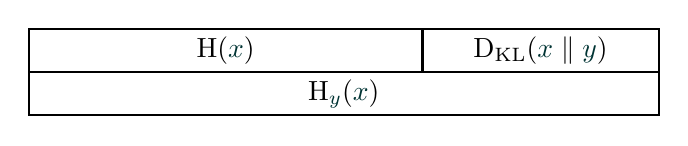
\begin{tikzpicture}
	\draw[thick] (0,0) rectangle (8,3.5ex) node[pos=.5] {$\H_{\rvar y}(\rvar x)$};
	\draw[thick] (0,3.5ex) rectangle (5,7ex) node[pos=.5] {$\H(\rvar x)$};
	\draw[thick] (5,3.5ex) rectangle (8,7ex) node[pos=.5] {$\Dkl{\rvar x}{\rvar y}$};
	\end{tikzpicture}
	\caption{Odnos entropije, unakrsne entropije i KL-divergencije.}
	\label{fig:dkl}
\end{figure}

\begin{figure}
	\centering
	\includegraphics[width=1.0\textwidth]{dkl-asymmetry}
	\caption{Asimetričnost KL-divergencije. $p$ je fiksna razdioba (funkcija gustoće), a $q*$ je Gaussova razdioba koja ju aproksimira minimizacijom KL-divergencije $\Dkl{q}{p}$ (lijevo) ili $\Dkl{p}{q}$ (desno). U donjem retku grafovi prikazuju podintegralne funkcije odgovarajućih KL-divergencija. Kod njih zbrojevi predznačenih površina obojanih područja odgovaraju KL-divergencijama $\Dkl{q}{p}$ (zeleno) ili $\Dkl{p}{q}$ (crveno). Optimalna aproksimirajuća razdioba desno ima veliku gustoću gdje god razdioba $p$ ima veliku gustoću. Lijevo optimalna aproksimirajuća razdioba nema veliku gustoću gdje razdioba $p$ nema veliku gustoću. Da je razmak između komponenata razdiobe $p$ malo manji, i lijeva razdioba $q^*$ bi pokrila oba moda i bila sličnija desnoj. Slika je napravljena po uzoru na sliku~3.6 u \citet{Goodfellow:2016:DL}.}
	\label{fig:dkl-asymmetry}
\end{figure}

\emph{Međusobna informacija} je mjera zavisnosti između slučajnih varijabli. Definirana je ovako:
\begin{align}
\I\del{\rvar x;\rvar y} \coloneqq \E_{\rvar x, \rvar y} \log_b\frac{P_{\rvar x, \rvar y}(x, y)}{P_{\rvar x}(x)P_{\rvar y}(y)} \text{,}
\label{eq:mutinf}
\end{align}
a može se i na ove načine izraziti:
\begin{align}
\I(\rvar x;\rvar y)
&= \H(\rvar x)+\H(\rvar y)-\H(\rvar x, \rvar y) \\
&= \H(\rvar x)-\H(\rvar x\mid \rvar y) \\ 
&= \H(\rvar y)-\H(\rvar y\mid\rvar x) \text{,}
\label{eq:mutinf2}
\end{align}
gdje je
\begin{align}
\H(\rvar x\mid \rvar y) \coloneqq \E_{\rvar x} \H(\rvar y\mid \rvar x=x)
\label{eq:condentropy}
\end{align}
\emph{uvjetna entropija}. Ako su $\rvar x$ i $\rvar y$ nezavisne, njihova međusobna informacija će biti $0$. Ako npr. postoji surjekcija $f$ tako da $\rvar y=f(\rvar x)$, tj. poznavanje ishoda varijable $\rvar x$ jednoznačno određuje ishod varijable $\rvar y$, onda $\H(\rvar y\mid\rvar x)=0$ i $\I(\rvar x;\rvar y) = \H(\rvar y)$. Ako je $f$ bijekcija, onda $\I(\rvar x;\rvar y) = \H(\rvar x) = \H(\rvar y)$. Definirane veličine mogu se prikazati kao na slici~\ref{fig:entropije}. Isti odnosi vrijede ako se entropija zamijeni diferencijalnom entropijom.

\begin{figure}
\centering
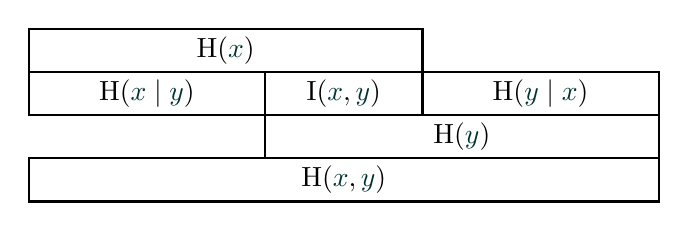
\begin{tikzpicture}
\draw[thick] (0,10.5ex) rectangle (5,14ex) node[pos=.5] {$\H(\rvar x)$};

\draw[thick] (0,7ex) rectangle (3,10.5ex) node[pos=.5] {$\H(\rvar x\mid\rvar y)$};	
\draw[thick] (3,7ex) rectangle (5,10.5ex) node[pos=.5] {$\I(\rvar x,\rvar y)$};
\draw[thick] (5,7ex) rectangle (8,10.5ex) node[pos=.5] {$\H(\rvar y\mid\rvar x)$};	
	
\draw[thick] (3,3.5ex) rectangle (8,7ex) node[pos=.5] {$\H(\rvar y)$};
\draw[thick] (0,0) rectangle (8,3.5ex) node[pos=.5] {$\H(\rvar x,\rvar y)$};
\end{tikzpicture}
\caption{Odnosi informacijsko-teorijskih veličina dviju slučajnih varijabli.}
\label{fig:entropije}
\end{figure}


\section{Optimizacija temeljena na gradijentu}

U ovom odjeljku su opisani osnovni optimizacijski algoritmi temeljeni na gradijentu i neki izvedeni algoritmi koji koriste doaatne heuristike. Oni su bitni u strojnom učenju (poglavlje \ref{chap:nsu}), posebno u dubokom učenju (poglavlje \ref{chap:dukm}). Primjena optimizacijskih algoritama u dubokom učenju opisana je u pododjeljku \ref{subsec:dukn-stoh-optimizacija}.

Neka je $\funcdef{f}{\R^n}{\R}$ funkcija čiji minumum s obzirom na parametre $\vec x$ želimo naći. Ona se u okolini točke $\vec x$, ako je dovoljno (beskonačno) puta derivabilna može izraziti Taylorovim redom:
\begin{align}
f(\vec x+\vec d) = f(\vec x) + \pd{}{\vec x}f(\vec x)\vec d + \frac{1}{2}\vec d^\tp{\tfrac{\partial^2y}{\partial\vec x\partial\vec x^\tp}}{\vec x}f(\vec x)\vec d + \cdots \text{.}
\end{align}
S drugačijim oznakama:
\begin{align} \label{eq:taylorov-red}
f(\vec x+\vec d) = f(\vec x) + \nabla_{\vec x}f(\vec x)^\tp\vec d + \frac{1}{2}\vec d^\tp\vec H_f(\vec x)\vec d + \cdots \text{.}
\end{align}

\subsection{Gradijentni spust i još neki algoritmi koje se temelje na njemu} \label{subsec:gradijenti-spust}

Ako je $\vec d$ ima malu normu, funkciju $f$ u okoline neke točke možemo dobro aproksimirati s prvih nekoliko članova Taylorovog reda. \emph{Gradijentni spust} je optimizacijski algoritam koji koristi linearnu aproksimaciju i iterativnim ažuriranjem parametara u smjeru gradijenta (\textit{najstrmijem} smjeru) traži minimum. Iteracija gradijentnog spusta ima ovakav oblik:
\begin{align} \label{eq:gs}
\vec x_i = \vec x_{i-1} - \eta\nabla_{\vec x}f(\vec x_{i-1}) \text{,}
\end{align}
gdje je $i$ redni broj iteracije, a $\eta$ \emph{veličina koraka} (\emph{stopa učenja} kod strojnog učenja) koja može biti konstanta ili može ovisiti o $i$.

Neka $\vec g=\nabla_{\vec x}f(\vec x)$ i $\vec H=\vec H_f(\vec x)$. Za dovoljno mal $\eta$
\begin{align} \label{eq:grad-delta-approx}
f(\vec x-\eta\vec g) = f(\vec x) - \eta\vec g^\tp\vec g - \frac{1}{2}\eta^2\vec g^\tp\vec H\vec g + \cdots
\end{align}
Uz neke blage uvjete koje mora zadovoljavati $f$ i dovoljno mal $\eta$, gradijentni spust konvergira, tj. proizvoljno se približi nekom lokalnom minimumu (ili stacionarnoj točki koja nije lokalni minimum, gdje $\nabla_{\vec x}f(\vec x)=\cvec 0$) ovisno o $\eta$. Jedan blagi uvjet može biti \emph{Lipschitz-kontinuiranost} funkcije $f$ ili njene derivacije \citep{Goodfellow:2016:DL}. Funkcija $f$ je Lipschitz-kontinuirana ako postoji konstanta $\lambda$ za koju za svaki par $(\vec x,\vec y)$ vrijedi:
\begin{align}
\envert{f(\vec x)-f(\vec y)} < \lambda\enVert{\vec x-\vec y} \text{.}
\end{align}
Najmanji takav $\lambda$ naziva se \emph{Lipschitzova konstanta}.

\subsubsection{Gradijentni spust s inercijom}

Jedna heuristika koja je često korisna kod optimizacije funkcija koje su nam zanimljive je simuliranje inercije. Jedan korak \emph{gradijentnog spusta s inercijom} (engl. \textit{momentum gradient descent}) ima ovakav oblik:
\begin{align}
\vec v_i &= \beta\vec v_{i-1} + \nabla_{\vec x}f(\vec x_{i-1}), \label{eq:gs-inercija-v}\\
\vec x_i &= \vec x_{i-1} - \eta\vec v_i \text{,}
\end{align}
gdje je $\beta\in\intco{0,1}$ faktor kojim se određuje \textit{otpor} proporcionalan \textit{brzini} $\vec v$, tj. otpor je proporcionalan faktoru $(1-\beta)$, što se bolje vidi ako se jednadžba~\eqref{eq:gs-inercija-v} izrazi ovako: 
\begin{align}
\vec v_i = \vec v_{i-1} - (1-\beta)\vec v_{i-1} + \nabla_{\vec x}f(\vec x_{i-1}) \text{.}
\end{align}
$\beta$ se obično odabire da bude bliže $1$. Uz $\beta=0$ dobiva se obični gradijentni spust, dobiva čestica koja klizi bez trenja. Uz dobro odabran $\beta$ prigušuju se pomaci koji nisu u smjeru gibanja $\vec v$. To omogućuje bržu konvergenciju i izbjegavanje malih lokalnih optimuma i drugih stacionarnih točaka. Svojstva gradijentnog spusta s inercijom su dobro objašnjena u \citet{GOH:2017:WMRW}.

Jedno poboljšanje gradijentnog spusta s inercijom je \emph{Nesterovljev postupak} \citep{Nesterov:2014:ILCOBC,Sutskever:2013:TRNN}:
\begin{align}
\vec v_i &= \beta\vec v_{i-1} + \nabla_{\vec x}f(\vec x_{i-1} - \eta\vec v_{i-1}), \\
\vec x_i &= \vec x_{i-1} - \eta\vec v_i \text{.}
\end{align}
Brzina se ažurira uz procjenu gradijenta u budućoj točki na temelju brzine iz prethodne iteracije. Onda se izračuna novi pomak uz tako ažuriranu brzinu.

\subsubsection{Primjeri algoritama koji koriste još neke heuristike}

Kod opisanih algoritama konvergenciju mogu usporavati područja u kojima gradijent ima male vrijednosti. Način na koji se ta pojava može poništiti je npr. da se gradijent podijeli s njegovom normom. Na taj način će pomaci ovisiti samo o stopi učenja, a ne o strmosti funkcije koja se minimizira. Algoritam \emph{RMSProp} (opisan npr. u \citet{Hinton:2012:NNMLLOMBG} ili \citet{Ruder:2016:OGDOA}) ostvaruje nešto slično. Iteracija RMSPropa izgleda ovako:
\begin{align}
\vec g_i &= \nabla_{\vec x}f(\vec x_{i-1}), \\
\vec r_i &= \rho\vec r_{i-1} + (1-\rho)\vec g_i^{\odot 2}, \\
\vec x_i &= \vec x_{i-1} - \eta\del{\epsilon\cvec 1+\vec r_i}^{\odot-\frac{1}{2}} \odot \vec g_i \text{,}
\end{align}
gdje je $\rho\in\intco{0,1}$ faktor koji određuje koliko se brzo ažurira pokretni prosjek gradijenta kvadriranog po elementima, a $\epsilon$ neka mala konstanta. $\rho$ se obično odabire da bude blizu $1$. Za $\rho=0$, ako se $\epsilon$ zanemari, dobiva se iteracija algoritma \emph{Rprop} \citep{Hinton:2012:NNMLLOMBG}: $\vec x_i = \vec x_{i-1} - \sgn\del{\nabla_{\vec x}f(\vec x_{i-1})}$. RMSPropu se još može dodati inercija.

Jedan algoritam koji često ubrzava učenje je \emph{Adam} \citep{Kingma:2014:AMSO}. On uključuje i inerciju i skaliranje. Ime Adam izvedeno je iz \textit{adaptive moment estimation}. Jedna iteracija tog algoritma izgleda ovako:
\begin{align}
\vec g_i &= \nabla_{\vec x}f(\vec x_{i-1}), \\
\vec v_i &= \beta_1\vec v_{i-1} + (1-\beta_1)\vec g_i, \\
\vec r_i &= \beta_2\vec r_{i-1} + (1-\beta_2)\vec g_i^{\odot 2}, \\
\vec v'_i &= \frac{1}{1-\beta_1^i}\vec v_i, \\
\vec r'_i &= \frac{1}{1-\beta_1^i}\vec r_i, \\
\vec x_i &= \vec x_{i-1} - \eta\del{\epsilon\cvec 1+\vec r_i^{\odot\frac{1}{2}}}^{\odot-1} \odot \nabla_{\vec x}f(\vec x_{i-1}) \text{,}
\end{align}
gdje je $\vec v_i$ pomični prosjek gradijenta, $\vec r_i$ pokretni prosjek kvadrata gradijenta po elementima, a $\epsilon$ mala konstanta. Parametar $\beta_1$ ima ulogu kao $\beta$ kao gradijentnog spusta s inercijom, a $\beta_2$ kao $\rho$ kod RMSPropa. Brzina $\vec v_i$ i pokretni prosjek kvadrata $\vec r_i$ se inicijaliziraju u $\cvec 0$ i u svakom koraku se skaliraju obrnuto proporcionalno udjelu gradijenta u odnosu na inicijalnu vrijednost $\cvec 0$ u pokretnom prosjeku radi poništavanja pristranosti procjena. Za velik $i$ ti faktori skaliranja približavaju se $1$.

\subsection{Postupci drugog reda}

Ovaj pododjeljak se temelji na \citet{Goodfellow:2016:DL}.

Ako koristimo kvadratnu aproksimaciju~\eqref{eq:grad-delta-approx}, možemo pokušati pronaći optimalni $\eta$ koji ju minimizira. $\eta$ za koji $\pd{}{\eta}f(\vec x-\eta\vec g)=0$ će, ako $\vec g^\tp\vec H\vec g>0$ dati minimum u smjeru gradijenta kvadratne aproksimacije funkcije $f$ u točki $\vec x$. Dobije se:
\begin{align}
\eta = \frac{\vec g^\tp \vec g}{\vec g^\tp\vec H\vec g} \text{.}
\end{align}
Ako je $\funcdef{f}{\R^n}{\R}$ konveksna (pozitivno definitna) kvadratna funkcija, izmijenjeni algoritam gradijentnog spusta, koji ovako određuje veličinu koraka, minimum pronalazi u najviše $n$ koraka. 

Postupak drugog reda koji se ne ograničava na pomake u smjeru gradijenta je \emph{Newton-Raphsonov postupak}. Deriviranjem desne strane jednadžbe~\eqref{eq:taylorov-red} po $\vec d$ i izjednačavanjem s $\cvec 0$ dobiva se:
\begin{align}
\cvec 0 = \nabla_{\vec x}f(\vec x)^\tp + \vec d^\tp\vec H_f(\vec x) + \cdots \text{.}
\end{align}
Uz kvadratnu aproksimaciju i kraće oznake $\vec g=\nabla_{\vec x}f(\vec x)$ i $\vec H=\vec H_f(\vec x)$: $\vec H\vec d = \vec g$. Slijedi da je pomak $\vec d$ koji daje stacionarnu točku aproksimacije
\begin{align}
\vec d = \vec H^{-1}\vec g \text{.}
\end{align}
Za nekvadratne funkcije, koje imaju pozitivno definitnu Hesseovu matricu u svakoj točki, može se iterativno primjenjivati
\begin{align}
\vec x_{i+1} = \vec x_i - \eta\vec H_f(\vec x_i)\nabla_{\vec x}f(\vec x_i)
\end{align}
s $\eta<1$.


\iffalse
\section{Računski grafovi}

Ovaj odjeljak definira \emph{računski graf} i opisuje grafički jezik za prikaz računskih grafova koji će se koristiti od poglavlja~\ref{chap:dukm}.

Računaski graf neke funkcije je usmjereni aciklički graf gdje čvorovi koji nemaju djecu predstavljaju varijable (parametre), ostali čvorovi predstavljaju operacije koje ovise varijablama ili rezultatima drugih operacija, a bridovi povezuju ulaze operacija s operacijama.

Ako je funkcija koju prikazujemo $f\colon x\mapsto y$ kompozicija $n$ funkcija: $f=f_n\circ\dots\circ f_2\circ f_1$, nju moćemo prikazati
\fi

\iffalse
\section{Pravila diferencijalnog računa}

\fi



\chapter{Statističko modeliranje}


\section{Probabilistički grafički modeli}

Neka su $\rvar x_1, .., \rvar x_n$ slučajne varijable čiju združenu razdiobu razmatramo. Želimo na temelju opežanih varijabli korištenjem pravila vjerojatnosti \emph{zaključivati} o razdiobama nekih neopažanih varijabli. Općenito, zaključivanje se provodi uvjetovanjem po opažanim varijablama i marginalizacijom po varijablama koje nas ne zanimaju izravno \citep{Murphy:2012:MLPP}:
\begin{align}
\p(\vec x_\text{q}\mid\vec x_\text{o}) 
= \frac{\p(\vec x_\text{q},\vec x_\text{o})}{\p(\vec x_\text{o})} 
= \frac{\int\p(\vec x_\text{q},\vec x_\text{n},\vec x_\text{o})\dif\vec x_\text{n}}{\int\p(\vec x_\text{q},\vec x_\text{n},\vec x_\text{o})\dif(\vec x_\text{q},\vec x_\text{n})} \text{.}
\label{eq:pgm-zakljucivanje-bayes}
\end{align}
Ovdje je $\rvec x_\text{q}$ niz varijabli o kojima želimo zaključivati (varijable upita), $\rvec x_\text{o}$ niz opažanih varijabli, a $\rvec x_\text{n}$ niz varijabli \textit{smetnje} (\textit{nuisance}).

Zavisnosti između slučajnih varijabli otežavaju modeliranje i zaključivanje -- potrebno je više podataka i zaključivanje je računski zahtjevnije. Obično možemo pretpostaviti uvjetne zavisnosti između slučajnih varijabli, što se može predstaviti neusmjerenim ili usmjerenim grafom. Prema definiciji na Wikipediji \footnote{\url{https://en.wikipedia.org/wiki/Graphical_model}}, \emph{probabilistički grafički model} ili \emph{grafički model} je probabilistički model koji se može prikazati grafom koji izražava strukturu uvjetnih zavisnosti među slučajnim varijablama. U tom grafu čvorovi označavaju slučajne varijable, a bridovi zavisnosti. Umjereni bridovi označavaju modeliranje uvjetne zavisnosti, a neusmjereni združeno modeliranje. Ako je graf grafičkog modela usmjeren i acikličan, on se naziva \emph{Bayesova mreža} ili \emph{Bayesovski model}, a ako je neusmjeren, naziva se \emph{Markovljeva mreža} ili \emph{Markovljevo slučajno polje} (engl. \textit{Markov random field}, \textit{MRF}). U nastavku ovog odjeljka naglasak će biti na Bayesovim mrežama.

Združena razdioba se prema pravilu umnoška (jednadžba~\eqref{eq:pravilo-umnoska}) može npr. ovako izraziti:
\begin{align}
\p(x_1,..,x_n) 
&= \p(x_1)\p(x_2\mid x_1)\cdots\p(x_n\mid x_1,..,x_{n-1}) \\
&= \prod_i\p(x_i\mid x_1,\bidot,x_{i-1}) \text{.}
\label{eq:pgm-pravilo-umnoska}
\end{align} 
Prema tome, svaki probabilistički grafički model ima ekvivalentnu Bayesovu mrežu. Ako uzmemo $n=4$, graf koji odgovara faktorizaciji u jednadžbi~\eqref{eq:pgm-pravilo-umnoska} prikazan je na slici~\ref{fig:bayesova-mreza}.

\begin{figure}
	\centering
	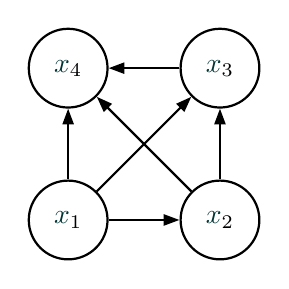
\begin{tikzpicture}
	\node[pnode] (x1) [] {$\rvar x_1$};
	\node[pnode] (x2) [right=of x1] {$\rvar x_2$};
	\node[pnode] (x3) [above=of x2] {$\rvar x_3$};
	\node[pnode] (x4) [above=of x1] {$\rvar x_4$};
	\path (x1) edge [dedge] (x2);	
	\path (x1) edge [dedge] (x3);	
	\path (x1) edge [dedge] (x4);
	\path (x2) edge [dedge] (x3);	
	\path (x2) edge [dedge] (x4);
	\path (x3) edge [dedge] (x4);	
	\end{tikzpicture}
	\caption{Prikaz grafičkog modela s faktorizacijom $\p(x_1,x_2,x_3,x_4)=\p(x_1)\p(x_2\mid x_1)\p(x_3\mid x_1,x_2)\p(x_4\mid x_1,x_2,x_3)$.}
	\label{fig:bayesova-mreza}
\end{figure}

Pretpostavljanjem uvjetnih nezavisnosti, neki bridovi grafa $G$ se mogu ukloniti pa za varijable (čvorove grafa) vrijedi \emph{uređajno Markovljevo svojstvo}:
\begin{align}
\rvar x\perp \pred_G(\rvar x) \setminus \pa_G(\rvar x) \mid \pa_G(\rvar x).
\end{align}
Jednadžba~\eqref{eq:pgm-pravilo-umnoska} onda prelazi u 
\begin{align}
\p(x_1,..,x_n) 
= \prod_i\p\del{x_i \midmid \bigcap_{\rvar x_j\in\pa_G(\rvar x_i)}\cbr{\rvar x_j=x_j}} \text{.}
\end{align} 
To omogućuje primjenu efikasnijih algoritama za zaključivanje \citep{Murphy:2012:MLPP}.
Na slici~\ref{fig:bm-kanonski} prikazani su osnovni slučajevi odnosa između triju slučajnih varijabli povezanih zavisnostima koje mogu biti dio većeg grafa. Oni su detaljnije objašnjeni npr. u \citet{Bishop:2006:PRML} i \citet{Alpaydin:2014:IML}. 

\begin{figure}
	\centering
	\begin{subfigure}[t]{0.48\textwidth}
		\centering
		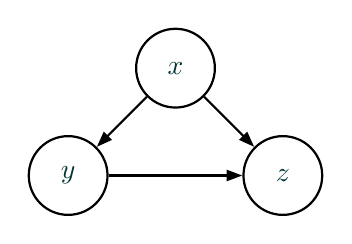
\begin{tikzpicture}
		\node[pnode] (x) [] {$\rvar x$};
		\node[pnode] (y) [below left=of x] {$\rvar y$};
		\node[pnode] (z) [below right=of x] {$\rvar z$};
		\path (x) edge [dedge] (y);	
		\path (x) edge [dedge] (z);
		\path (y) edge [dedge] (z);
		\end{tikzpicture}
		\caption{Grafički model s faktorizacijom $\p(x,y,z) = \p(x)\p(y\mid x)\p(z\mid x,y)$.}
		\label{subfig:bm-kanonski-a}
	\end{subfigure}
	~
	\begin{subfigure}[t]{0.48\textwidth}
		\centering
		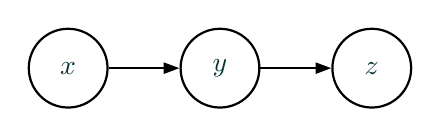
\begin{tikzpicture}
		\node[pnode] (x) [] {$\rvar x$};
		\node[pnode] (y) [right=of x] {$\rvar y$};
		\node[pnode] (z) [right=of y] {$\rvar z$};
		\path (x) edge [dedge] (y);	
		\path (y) edge [dedge] (z);
		\end{tikzpicture}
		\caption{Uz $\rvar x\perp\rvar z\mid\rvar y$ faktorizacija postaje $\p(x,y,z) = \p(x)\p(y\mid x)\p(z\mid y)$ (lanac).}
		\label{subfig:bm-kanonski-head-to-tail}
	\end{subfigure}
	\vskip\baselineskip
	\begin{subfigure}[t]{0.48\textwidth}
		\centering
		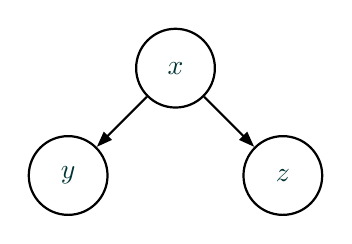
\begin{tikzpicture}
		\node[pnode] (x) [] {$\rvar x$};
		\node[pnode] (y) [below left=of x] {$\rvar y$};
		\node[pnode] (z) [below right=of x] {$\rvar z$};
		\path (x) edge [dedge] (y);	
		\path (x) edge [dedge] (z);
		\end{tikzpicture}
		\caption{Uz $\rvar y\perp\rvar z\mid\rvar x$ faktorizacija postaje $\p(x,y,z) = \p(x)\p(y\mid x)\p(z\mid x)$ (račvanje).}
		\label{subfig:bm-kanonski-tail-to-tail}
	\end{subfigure}
	~
	\begin{subfigure}[t]{0.48\textwidth}
		\centering
		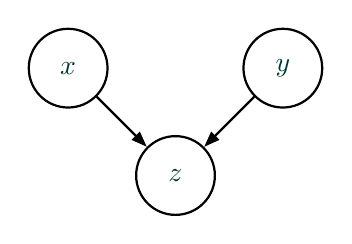
\begin{tikzpicture}
		\node[pnode] (z) [] {$\rvar z$};
		\node[pnode] (x) [above left=of z] {$\rvar x$};
		\node[pnode] (y) [above right=of z] {$\rvar y$};
		\path (x) edge [dedge] (z);	
		\path (y) edge [dedge] (z);
		\end{tikzpicture}
		\caption{Uz $\rvar x\perp\rvar y$ faktorizacija postaje $\p(x,y,z) = \p(x)\p(y)\p(z\mid x,y)$ (sraz). Ovdje također vrijedi $\rvar x\not\perp\rvar y\mid \rvar z$.}
		\label{subfig:bm-kanonski-head-to-head}
	\end{subfigure}
	\caption{Osnovni slučajevi uvjetne nezavisnosti. Slike \subref{subfig:bm-kanonski-head-to-tail}, \subref{subfig:bm-kanonski-tail-to-tail} i \subref{subfig:bm-kanonski-head-to-head} prikazuju grafove dobivene uvođenjem pretpostavki uvjetne nezavisnosti za grafički model s $3$ slučajne varijable prikazan na slici \subref{subfig:bm-kanonski-a}.}
	\label{fig:bm-kanonski}
\end{figure}

Na slici~\ref{fig:bm-regresija} prikazan je primjer na kojem se koriste još neke oznake: sivi čvorovi označavaju opažane varijable, četverokut označava veći broj podgrafova s istom strukturom.

\begin{figure}
	\centering
	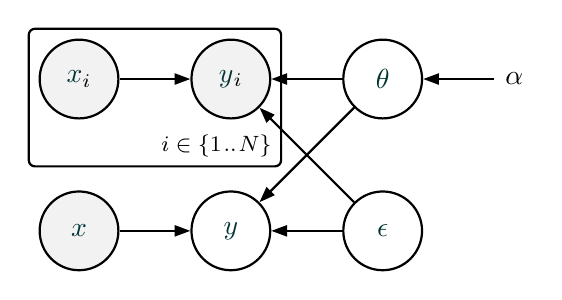
\begin{tikzpicture}
	\node[pnode] (t) [] {$\rvec \theta$};
	\node[textnode] (a) [right=of t] {$\alpha$};
	\node[pnode] (e) [below=of t] {$\rvar\epsilon$};
	\node[greypnode] (yi) [left=of t] {$\rvar y_i$};
	\node[greypnode] (xi) [left=of yi] {$\rvec x_i$};
	\node[pnode] (y) [left=of e] {$\rvar y$};	
	\node[greypnode] (x) [left=of y] {$\rvec x$};
	\path (a) edge [dedge] (t);	
	\path (t) edge [dedge] (yi);	
	\path (t) edge [dedge] (y);
	\path (e) edge [dedge] (yi);	
	\path (e) edge [dedge] (y);
	\path (xi) edge [dedge] (yi);
	\path (x) edge [dedge] (y);
	\plate{}{(xi)(yi)}{$i \in \cbr{1\bidot N}$};
	\end{tikzpicture}
	\caption{Primjer grafičkog modela s faktorizacijom 
		$\p(\vec x, y,\vec x_1\bidot\vec x_N,y_1\bidot y_N,\vec\theta,\epsilon) 
		= \p(\vec\theta)\p(\epsilon)p_{\rvec x}(\vec x)p_{\rvec y\mid\rvec x,\rvec\theta,\rvar\epsilon}(y\mid\vec x,\vec\theta,\epsilon) \prod_i\del{p_{\rvec x}(\vec x_i)p_{\rvec y\mid\rvec x,\rvec\theta,\rvar\epsilon}(y_i\mid\vec x_i,\vec\theta,\epsilon)}$. Graf prikazuje model regresije, gdje su $\rvec\theta$ nepoznati parametri, $\rvec x_i$ i $\rvec y_i$ opažani parovi ulaza i izlaza, $\rvec x$ opažani ulaz s nepoznati izlazom, a $\rvar\epsilon$ homoskedastički šum, tj. šum koji ne ovisi o ulazu. Na slici je još eksplicitno prikazana deterministička varijabla $\alpha$ koja je parametar razdiobe $\p(\rvec\theta)=\p(\rvec\theta\mid\alpha)$. Slika je napravljena po uzoru na sliku~14.7 u \citet{Alpaydin:2014:IML}.}
	\label{fig:bm-regresija}
\end{figure}

Općenitije, o uvjetnoj nezavisnosti podskupova varijabli govori svojstvo \emph{d-separacije}. Kažemo da je staza (podgraf sa strukturom lanca) $P$ grafa $G$ \emph{d-odvojena} skupom čvorova $\set E$ akko $P$ sadrži barem jedno od sljedećeg \citep{Murphy:2012:MLPP}:
\begin{enumerate}
	\item lanac $\rvar a\rightarrow\rvar b\rightarrow\rvar c$, gdje $\rvar b\in E$
	\item račvanje $\rvar a\leftarrow\rvar b\rightarrow\rvar c$, gdje $\rvar b\in E$
	\item sraz $\rvar a\rightarrow\rvar b\leftarrow\rvar c$, gdje $\forall \rvar b'\in\cbr{\rvar b}\cup\succ_G(\rvar b), \rvar b'\notin E$.
\end{enumerate}
Kažemo da skup čvorova $\set E$ d-odvaja čvorove $\rvar x$ i $\rvar y$ akko su sve staze između njih d-odvojene. Vrijedi $\rvar x\perp\rvar y \mid \set E$ akko skup čvorova $\set E$ d-odvaja čvorove $\rvar x$ i $\rvar y$. To se može poopćiti na skupove čvorova. Skup čvorova opažanjem kojega neki čvor postaje neovisan o ostatku grafa naziva se \emph{Markoveljev pokrivač} (engl. \textit{Markov blanket}). Markovljev pokrivač čvora $\rvar x$ je
\begin{align}
\pa_G(\rvar x)\cup\ch_G(\rvar x)\cup\bigcup_{\rvar y\in\ch_G(\rvar x)}\pa_G(\rvar y)
\end{align}

U navedenim knjigama opisani su algoritmi koji se koriste za efikasno zaključivanje iskorištavanjem strukture grafa.


\section{Procjena parametara i zaključivanje}

\subsection{Procjenitelji i točkaste procjene parametara}

Ovaj pododjeljak se temelji na \citet{Elezovic:2007:VSSV}.

Neka je $\rvar x$ slučajna varijabla i $\p(\rvar x)$ njena razdioba s nama nepoznatim parametrom $\theta$. Taj parametar možemo procijeniti na temelju opaženih vrijednosti $x_1,..,x_n$ slučajne varijable $\rvar x$, za što definiramo funkciju $g$ koja daje procjenu parametara
\begin{align}
\hat{\theta}=f(x_1,..,x_N) \text{.}
\end{align}
Ako kao parametre takve funkcije uzmemo \emph{uzorak}, tj. skup slučajnih varijabli $\rset D=\del{\rvar x_1,..,\rvar x_N}$, gdje pretpostavljamo da su $\rvar x_1,..,\rvar x_N$ međusobno nezavisne i imaju istu razdiobu kao $\rvar x$, dobivamo slučajnu varijablu
\begin{align}
\hat{\rvar\theta}=f(\rset D) \text{.}
\end{align}
Takva slučajna varijabla naziva se \emph{statistika}. Ako je $\theta$ nepoznati parametar razdiobe $\p(\rvar x)$, onda kažemo da je ta statistika $\hat{\rvar\theta}$ \emph{procjenitelj} parametra $\theta$, a njen ishod $\hat{\theta}$ \emph{procjena} parametra $\theta$.

\subsection{Svojstva i pogreška procjenitelja}

\emph{Pristranost} procjenitelja $\hat{\rvar\theta}$ je definirana izrazom $\E\hat{\rvar\theta} - \theta$, gdje je $\theta$ stvarna vrijednost parametra koji se procjenjuje. Ona mjeri koliko procjenitelj griješi neovisno o ishodu uzorka. Kažemo da je procjenitelj parametra $\theta$ \emph{nepristran} ako vrijedi
\begin{align}
\E\hat{\rvar\theta} = \theta \text{.}
\end{align}

\emph{Varijanca} procjenitelja $\hat{\rvar\theta}$ je definirana izrazom $\D\hat{\rvar\theta}$. Ona mjeri koliko procijenitelj griješi ovisno variranju uzorka. 
%Neka je $\rset D$ uzorak od $n$ slučajnih varijabli. Ako su $\hat{\rvar\theta}_1(\rset D)$ i $\hat{\rvar\theta}_2(\rset D)$ dva nepristrana procjenitelja za $\theta$, kažemo da je $\hat{\rvar\theta}_1$ \emph{bolji} od $\hat{\rvar\theta}_2$ ako
%\begin{align}
%\D \hat{\rvar\theta}_1 < \D\hat{\rvar\theta}_2 \text{.}
%\end{align}
Neka $N$ u oznaci ${\rset D}_N$ označava veličinu uzorka. Nepristrani procjenitelj $\hat{\rvar\theta}$ je \emph{valjan} ako 
\begin{align}
\lim_{N\to\infty} \D\sbr{\hat{\rvar\theta}(\rset D_N)} = 0  \text{.}
\end{align}

Može se pokazati da je očekivanje srednje kvadratne pogreške procjenitelja jednaka zbroju njegove varijance i kvadrata njegove pristranosti \citep{Snajder:2014:SU}, tj. 
\begin{align}
\E\sbr{\del{\hat{\rvar\theta}-\theta}^2} = \D\hat{\rvar\theta} + \del{\E\hat{\rvar\theta}}^2  \text{.}
\end{align}

\subsection{Procjenitelj maksimalne izglednosti}

\emph{Procjenitelj maksimalne izglednosti} (\emph{ML-procjenitelj}, engl. \textit{maximum likelihood}) uzorku dodjeljuje parametre maksimiziraju vjerojatnost uzorka, tj. imaju najveću \emph{izglednost}:
\begin{align}
\rvec\theta_\text{ML} = \argmax_{\vec\theta} \p(\rset{D}\mid\vec\theta) \text{.}
\end{align}
Zbog pretpostavke međusobne nezavisnosti primjera vrijedi
\begin{align}
 \p(\set{D}\mid\vec\theta) = \prod_{\vec d\in\set{D}} \p(\vec d\mid\vec\theta) \text{.}
\end{align}

Za razliku od generativnih, diskriminativni modeli ne modeliraju razdiobu ulaznih primjera, nego samo uvjetnu razdiobu $\p(\vec y\mid \vec x, \set{D})$ pa kod njih razdioba ulaznih primjera ne ovisi o $\vec\theta$, tj. $\p(\vec x\mid\vec\theta) = \p(\vec x)$. Onda je izglednost
\begin{align}\label{eq:izglednost-diskr}
\p(\set{D}\mid\vec\theta) 
= \prod_{(\vec x,\vec y)\in\set{D}} \p(\vec y\mid\vec x,\vec\theta)\p(\vec x\mid\vec\theta) 
= \p(\vec x) \prod_{(\vec x,\vec y)\in\set{D}} \p(\vec y\mid\vec x,\vec\theta) \text{.}
\end{align}
Faktor $\p(\vec x)$ ne ovisi o parametrima i može se zanemariti pri optimizaciji.

\subsection{Procjenitelj maksimalne aposteriorne vjerojatnosti}

\emph{Procjenitelj maksimalne aposteriorne vjerojatnosti} (\emph{MAP-procjenitelj}, engl. \textit{maximum a posteriori estimator}) u obzir uzima \emph{apriornu razdiobu} $\p(\rvec\theta)$ koja predstavlja dodatne pretpostavke za razdiobu parametara. Apriorna razdioba parametara pojednostavljuje model dajući prednost nekim hipotezama i posebno je korisna kada ima malo podataka. Apriorna razdioba može biti definirana nekim hiperparametrima ali oni ovdje nisu prikazani. Po Bayesovom pravilu, \emph{aposteriorna vjerojatnost} parametara je
\begin{equation} \label{eq:posterior-bayes}
\p(\vec\theta\mid\set D) 
 = \frac{\p(\set{D}\mid\vec\theta)\p(\vec\theta)}{\p(\set{D})}
 = \frac{\p(\set{D}\mid\vec\theta)\p(\vec\theta)}{\int \p(\set{D}\mid\vec\theta')\p(\vec\theta')\dif\vec\theta'} \text{.}
\end{equation}
Maksimizacijom aposteriorne vjerojatnosti dobivaju se parametri
\begin{equation}
 \rvec\theta_\text{MAP} = \argmax_{\vec\theta} \p(\vec\theta\mid\rset D) = \argmax_{\vec\theta} \p(\rset{D}\mid\vec\theta)\p(\vec\theta) \text{.}
\end{equation}
Ovdje nije potrebno normalizirati aposteriornu vjerojatnost izračunavanjem \emph{marginalne izglednosti} (engl. \textit{marginal likelihood}, \textit{evidence}) $\p(\set{D})$ u nazivniku na desnoj strani jednadžbe~\eqref{eq:posterior-bayes} jer ona ne ovisi $\vec\theta$, nego samo o modelu $\set H$. Odabirom uniformne (neinformativne) apriorne razdiobe MAP-procjenitelj postaje ekvivalentan ML-procjenitelju.

Poželjno je da $\p(\set{D}\mid\vec\theta)$ i $\p(\vec\theta)$ kao funkcije parametra $\vec\theta$ imaju takav algebarski oblik da njihov umnožak ima sličan oblik i može se analitički izračunati. Ako $\p(\rvec\theta)$ i $\p(\rvec\theta\mid\set D)$ imaju isti algebarski oblik, nazivaju se \emph{konjugatne razdiobe} \citep{Snajder:2014:SU}.
% TODo ^^

\subsection{Bayesovski procjenitelj i zaključivanje}

Prethodno opisani procjenitelji daju točkastu procjenu parametara i ne izražavaju nesigurnost procjene kojoj uzrok može biti npr. nedovoljna količina podataka ili šum u podacima za učenje. \emph{bayesovski procjenitelj} kao procjenu daje razdiobu nad hipotezama $\p(\rvec\theta\mid\set D)$ za koju je integriranjem po svim mogućim parametrima potrebno izračunati marginalnu izglednost $\p(\set{D})=\int\p(\set{D}\mid\vec\theta')\p(\vec\theta')\dif{\vec\theta'}$ iz nazivnika na desnoj strani jednadžbe~\eqref{eq:posterior-inference}. 

Kod složenijih modela često ne možemo odabrati konjugatnu apriornu razdiobu, a i funkcija izglednosti je sama po sebi već dovoljno složena da se, neovisno o apriornoj razdiobi, marginalna izglednost $\p(\set{D})$ ne može ni analitički ni numerički traktabilno računati. 

Vjerojatnost nekog primjera $\vec d$ procjenjuje se marginalizacijom po parametrima \citep{Neal:1995:BLNN}:
\begin{align}
\p(\vec d\mid\set D) 
= \int\p(\vec d\mid\vec\theta)\p(\vec\theta\mid\set D) \dif{\vec\theta}
= \E_{\rvec\theta\mid\set D}\p(\vec d\mid\rvec\theta) \text{,}
\end{align}
gdje je korištena uvjetna nezavisnost $\rvec d\perp\rset D\mid\rvec\theta$.

Kada se parametri točkasto procjenjuju, npr. MAP-procjeniteljem, točkasta procjena parametara $\hat{\vec\theta}$ aproksimira cijelu aposteriornu razdiobu, tj. $\p(\vec\theta\mid\set{D}) \approx \dirac(\hat{\vec\theta}-\vec\theta)$. Onda je
\begin{align}
\p(\vec d\mid\set D) 
\approx \int\p(\vec d\mid\vec\theta) \dirac(\hat{\vec\theta}-\vec\theta) \dif{\vec\theta} 
=\p(\vec d\mid\hat{\vec\theta}) \text{.}
\end{align}

Za diskriminativne modele se bayesovsko zaključivanje može izraziti ovako:
\begin{align*}
\p(\vec y\mid \vec x, \set{D})
&= \frac{\p(\vec x,\vec y\mid\set{D})}{\p(\vec x\mid\set{D})} \\
&= \frac{\int\p(\vec y\mid \vec x,\vec\theta)\p(\vec x\mid\vec\theta) \p(\vec\theta\mid\set D) \dif{\vec\theta}}{\int\p(\vec x\mid\vec\theta)\p(\vec\theta\mid\set D)\dif{\vec\theta}} \\
&= \frac{\p(\vec x)\int\p(\vec y\mid \vec x,\vec\theta)\p(\vec\theta\mid\set D) \dif{\vec\theta}}{\p(\vec x)\int\p(\vec\theta\mid\set D)\dif{\vec\theta}} \text{.}
\end{align*}
Poništavanjem $\p(\vec x)$ i integriranjem nazivnika dobiva se
\begin{align}
\p(\vec y\mid \vec x, \set{D})
= \int\p(\vec y\mid \vec x,\vec\theta)\p(\vec\theta\mid\set D) \dif{\vec\theta}
= \E_{\rvec\theta\mid\set D}\p(\vec y\mid\vec x,\rvec\theta) \text{.}
\end{align}

Kod regresije je često, ako pretpostavljamo da pogreška izlaza ima Gaussovu razdiobu, najbolja procjena hipoteze očekivanje po naučenoj razdiobi parametara \citep{Neal:1995:BLNN}: 
\begin{align}
h(\vec x)
= \E_{\rvec\theta\mid\set D} h(\vec x; \rvec\theta)
= \int h(\vec x; \vec\theta)\p(\vec\theta\mid\set D) \dif{\vec\theta} \text{.}
\end{align}
U tom slučaju se nesigurnost može izraziti disperzijom
 $\D_{\rvec\theta\mid\set D} h(\vec x; \rvec\theta)$.

 
\section{Monte Carlo aproksimacija}

Ovaj odjeljak se temelji na \citet{Goodfellow:2016:DL}.

\emph{Monte Carlo aproksimacija} je postupak procjenjivanja vrijednosti koje se mogu izraziti kao očekivanje neke funkcije neke slučajne varijable na temelju uzoraka. Ponekad nije moguće analitički ili numerički traktabilno ili efikasno izračunati neki integral (ili zbroj). Ako se on može ovako izraziti:
\begin{align}
s = \int\p(x)f(x)\dif x = \E f(\rvar x) \text{,}
\end{align}
može se procijeniti uzorkovanjem:
\begin{align}
\hat{\rvar s}_n = \frac{1}{n}\sum_{i=1}^n f(\rvar x_i) \text{.}
\end{align}
Procjenitelj $\hat{\rvar s}_n$ je nepristran ako su $\rvar x_i$ nezavisne i imaju istu razdiobu kao $\rvar x$ i valjan ako su varijance $f(\rvar x_i)$ ograničene. Vrijedi $\D\hat{\rvar s}_n = \frac{1}{n} \D f(\rvar x)$.

U širem smislu, postupci \textit{Monte Carlo} obuhvaćaju i generiranje uzoraka slučajne varijable čije se očekivanje procjenjuje.


\section{Aproksimacija razdioba i aproksimacijsko zaključivanje}

Ovaj odjeljak se uglavnom temelji na \citet{Blei:2017:VIRS} i malo na \citet{Yang:2017:UVLB}.

Važan problem u bayesovskoj statistici, gdje se zaključivanje temelji na izračunima koji uključuju aposteriornu razdiobu, je aproksimacija razdioba koje su zahtjevne za računanje. Kod složenijih Bayesovskih modela aposteriorna razdioba se ne može lako izračunati i treba koristiti aproksimacijske postupke od kojih su glavni \emph{varijacijski} postupci \citep{Jordan:1999:IVMGM} i postupci \emph{Monte Carlo} aproksimacije s uzorkovanjem pomoću \emph{Markovljevog lanca} (MCMC, engl. \textit{Markov chain Monte Carlo}). MCMC-postupci temelje se na definiranju stohastičkog procesa koji ima stacionarnu razdiobu jednaku razdiobi koja se aproksimira, omogućuju asimptotski egzaktno uzorkovanje velike klase razdioba. Varijacijski postupci temelje se na aproksimaciji razdiobe nekom jednostavnijom koja se pronalazi rješavanjem optimizacijskog problema, brži su i jednostavniji za ostvariti za složenije modele.

Razmatramo bayesovski model koji ima latentnu varijablu $\rvec z$ i vidljivu varijablu $\rvec x$. Model je prikazan na slici~\ref{fig:pgmzx} i opisan je ovom jednadžbom združene vjerojatnosti:
\begin{align*}
\p(\vec x, \vec z) = \p(\vec z)\p(\vec x\mid\vec z) \text{.}
\end{align*}
Zaključivanjem se određuje aposteriorna razdioba latentne varijable:
\begin{align} \label{eq:posterior-inference}
\p(\vec z\mid\vec x) = \frac{\p(\vec x,\vec z)}{\p(\vec x)} = \frac{\p(\vec x,\vec z)}{\int\p(\vec x, \vec z) \dif{\vec z}} \text{.}
\end{align}
na temelju opažanih vrijednosti slučajne varijable $\rvec x$ (podataka). Kod složenijih modela integriranje marginalne izglednosti u nazivniku nije traktabilno i aposteriorna razdioba se mora aproksimirati \emph{približnim (aproksimacijskim) zaključivanjem}.

\begin{figure}
	\centering
	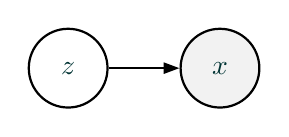
\begin{tikzpicture}
	\node[pnode] (z) [] {$\rvec z$};
	\node[greypnode] (x) [right=of z] {$\rvec x$};
	\path (z) edge [dedge] (x);
	\end{tikzpicture}
	\caption{Prikaz grafičkog modela sa skrivenom varijablom $\rvec z$ i opažanom varijablom $\rvec x$.}
	\label{fig:pgmzx}
\end{figure}


%\section{Postupci uzorkovanja}
%TODO
%1.3.1 \citet{Neal:1995:BLNN}.


\section{Varijacijsko zaključivanje}

Za razliku od uzorkovanja kod MCMC-postupaka, osnovna ideja kod varijacijskog zaključivanja je optimizacija. Prvo se odabire familija razdioba $\set{Q}=\cbr{\p(\tilde{\rvec z})}_{\tilde{\rvec z}}=\cbr{q_{\vec\phi}}_{\vec\phi}$ koje su lakše za računanje. Razdiobe iz $\set{Q}$ su parametrizirane tzv. \emph{varijacijskim parametrima} $\vec\phi$. Cilj je na temelju podataka kao zamjenu za aposteriornu razdiobu $\p(\vec z\mid\vec x)$ pronaći razdiobu iz $\set{Q}$ koja ju što bolje aproksimira. To možemo ostvariti minimizacijom Kullback-Leiblerove (KL) divergenciju s obzirom na stvarnu aposteriornu razdiobu po varijacijskim parametrima $\vec\phi$:
\begin{align}
q^* = \argmin_{\p(\tilde{\rvec z})\in\set Q} \Dkl{\tilde{\rvec z}}{(\rvec z\mid\vec x)} \text{.}
\end{align}
Naziv \emph{varijacijsko zaključivanje} dolazi od varijacijskog računa\footnote{\url{https://en.wikipedia.org/wiki/Calculus_of_variations}}, gdje se koriste varijacije, tj. male promjene u funkcijama i funkcionalima, kako bi se pronašli minimumi ili maksimumi funkcionala, preslikavanja iz skupa funkcija u $\R$, koji su često izraženi kao integrali koji uključuju funkcije i njihove derivacije.

Neka je $q$ oznaka funkcije gustoće vjerojatnosti aproksimacijske razdiobe: $q\coloneqq p_{\tilde{\rvec z}}$. Ako ciljnu funkciju ovako izrazimo:
\begin{align}
\Dkl{\tilde{\rvec z}}{(\rvec z\mid\vec x)} 
&= \E_{\tilde{\rvec z}} \ln\frac{q(\tilde{\vec z})}{p_{\rvec z\mid x}(\tilde{\vec z})} \nonumber \\
&= \E_{\tilde{\rvec z}}\ln q(\tilde{\vec z}) - \E_{\tilde{\rvec z}}\ln \p(\rvec z=\tilde{\vec z},\vec x) + \ln\p(\vec x) \text{,} \label{eq:dkl-split}
\end{align}
vidi se da se ona ne može lako izračunati jer zahtijeva računanje marginalne izglednosti $\p(\vec x)$ iz nazivnika u jednadžbi~\eqref{eq:posterior-inference} marginalizacijom po $\rvec z$. Marginalna izglednost ne ovisi o varijacijskim parametrima pa ju možemo zanemariti i maksimiziramo funkciju koja se naziva \emph{varijacijska donja granica} (engl. \textit{variational lower bound}) ili \emph{donja granica (logaritma) marginalne izglednosti} (engl. \textit{(log) evidence lower bound}, \textit{ELBO}):
\begin{align}
L_{\vec x}(\tilde{\rvec z}) 
\coloneqq \ln\p(\vec x) - \Dkl{\tilde{\rvec z}}{(\rvec z\mid\vec x)}
= \E_{\tilde{\rvec z}} \ln \p(\rvec z=\tilde{\vec z},\vec x) - \E_{\tilde{\rvec z}} \ln q(\tilde{\vec z})  \text{.} \label{eq:elbo}
\end{align}
Ona se može i ovako izraziti:
\begin{align}
L_{\vec x}(\tilde{\rvec z}) 
= \E_{\tilde{\rvec z}} \ln\p(\vec x\mid\rvec z=\tilde{\vec z}) - \Dkl{\tilde{\rvec z}}{\rvec z}  \text{.}
\end{align}
Maksimiziranje takve ciljne funkcije s obzirom na varijacijske parametre daje razdiobu $q^*=\p(\tilde{\rvec z}^*)$ koja dobro objašnjava podatke jer se potiče veće očekivanje logaritma izglednosti (prvi član), a ne razlikuje se previše od apriorne razdiobe jer se potiče manja KL-divergencija između varijacijske razdiobe i apriorne razdiobe \citep{Gal:2015:DBAA}.

Naziv \textit{donja granica marginalne izglednosti} dolazi od toga što su \citet{Jordan:1999:IVMGM} izveli nejednakost $\ln\p(\vec x) \geq L_{\vec x}(\tilde{\rvec z})$ preko Jensenove nejednakosti. Ta nejednakost slijedi i iz prethodne jednadžbe i nenegativnosti KL-divergencije:
\begin{align}
\ln\p(\vec x) = L_{\vec x}(\tilde{\rvec z}) + \Dkl{\tilde{\rvec z}}{(\rvec z\mid\rvec x)} \geq L_{\vec x}(\tilde{\rvec z}) \text{.}
\end{align}

\subsection{Metoda polja sredina}

Dodatno pojednostavljenje koje pomaže u modeliranju i optimizaciji je pretpostavljanje nezavisnosti između latentnih varijabli. Onda za varijacijsku razdiobu vrijedi ovakva faktorizacija:
\begin{align}
q(\tilde{\vec z}) = \prod_i q_i(\tilde{z}_i),
\end{align}
gdje su $q_i$ funkcije gustoće pojedinih slučajnih varijabli, a $\tilde{z}_i=\tilde{\vec z}_\ind{i}$. Kod \emph{metode polja sredina} pretpostalja se takva razdioba i obično se primjenjuje koordinatni spust za optimizaciju, s čime ima veze ime metode. To je detaljnije objašnjeno u \citet{Murphy:2012:MLPP}.

\iffalse
Neka je, radi kraćeg zapisa, $t(\tilde{\vec z}) \coloneqq \p(\rvec z=\tilde{\vec z},\rvec x=\vec x)$. Uz aproksimaciju polja sredina donja varijacijska granica postaje
\begin{align}
L_{\vec x}(\tilde{\rvec z}) 
&= \E_{\tilde{\rvec z}}\sbr{\ln t(\tilde{\vec z}) - \ln q(\tilde{\vec z})}
\\
&= \int\dif{\tilde{\vec z}} \del{\prod_i q_i(\tilde{z}_i)}\del{\ln t(\tilde{\vec z}) - \sum_j \ln q_j(\tilde{z}_j)}
\text{.}
\end{align}
\fi



\chapter{Nadzirano strojno učenje} \label{chap:nsu}

Ovo poglavlje se uglavnom temelji na \citet{Snajder:2014:SU} i \citet{Goodfellow:2016:DL}.

Zadatak algoritama \emph{nadziranog učenja} je preslikavanje \emph{ulaznih primjera} $\vec x$ iz \emph{ulaznog prostora} $\set{X}$ u \emph{izlaze} (\emph{oznake}) $\vec y\in\set{Y}$ na temelju konačnog skupa označenih primjera $\set{D} = \cbr{\del{\vec x_i,\vec y_i}}_{i}$. Algoritmima strojnog učenja pretražuje se \emph{model} ili \emph{prostor hipoteza} u cilju pronalaska \emph{hipoteze} koja osim primjera iz skupa za učenje, u izlaze dobro preslikava i primjere koji nisu u skupu za učenje. Sposobnost postizanja dobre performanse na neviđenim primjerima naziva se \emph{generalizacija}.

Neka je $\set{D}=\cbr{\vec d_i}_i$ skup nezavisnih primjera izvučenih iz neke razdiobe $\distrib{D}$. Možemo definirati \emph{probabilistički model} $\set H$ s nepoznatim parametrima $\vec\theta$ kojem je cilj što bolje modelirati tu razdiobu pronalaskom najbolje hipoteze na temelju podataka: $\p(\vec{d}\mid\set{D},\set H)$. Model koji modelira razdiobu primjera nazivamo \emph{generativnim modelom}. U nastavku ćemo izostavljati oznaku modela radi kraćeg zapisa.

Ako su primjeri parovi $\vec d_i = \del{\vec x_i, \vec y_i} \in \set{X}\times\set{Y}$, može nam biti cilj ulaznim primjerima iz $\set{X}$ dodjeljivati oznake iz $\set Y$. Ako je problem koji rješavamo dodjeljivanje oznaka ulaznim primjerima, onda su često prikladniji \emph{diskriminativni modeli}. Probabilistički diskriminativni modeli izravno modeliraju uvjetne razdiobe $\p(\rvec y\mid \vec x)$ hipotezom koja ulazni primjer $\vec x$ preslikava u razdiobu $\p(\rvec y\mid\vec x,\set{D})$. Neprobabilistički diskriminativni modeli modeliraju funkciju dodjeljivanja oznaka hipotezom $\funcdef{h}{\set{X}}{\set{Y}}$. Modeliranje zajedničke razdiobe $\p(\rvec x,\rvec y)$ obično zahtijeva više računalnih resursa i podataka \citep{Bishop:2006:PRML}.

Modeli se još mogu podijeliti na \emph{parametarske} i \emph{neparametarske}. Kod parametarskih modela broj parametara je unaprijed određen, dok kod neparametarskih on ovisi o podacima za učenje.


\section{Induktivna pristranost}

Uz zadani skup hipoteza koji dopušta model, \emph{algoritam strojnog učenja} traži parametre koji definiraju jednu hipotezu. Učenje hipoteze je loše definiran (engl. \textit{ill-posed}) problem jer skup podataka $\set{D}$ nije dovoljan za jednoznačan odabir hipoteze. Osim dobrog opisivanja podataka za učenje, naučena hipoteza mora dobro generalizirati. Kako bi učenje i generalizacija bili mogući, potreban je skup pretpostavki koji se naziva \emph{induktivna pristranost}. Razlikujemo dvije vrste induktivne pristranosti \citep{Snajder:2014:SU}:
\begin{enumerate}[topsep=0pt,itemsep=0pt,partopsep=0pt]
	\item \emph{pristranost ograničavanjem} ili \emph{pristranost jezika} -- ograničavanje skupa hipoteza koje se mogu prikazati modelom,
	\item \emph{pristranost preferencijom} ili \emph{pristranost pretraživanja} -- dodjeljivanje različitih prednosti različitim hipotezama.
\end{enumerate}
Većina algoritama strojnog učenja kombinira obje vrste induktivne pristranosti. 


\section{Komponente algoritma strojnog učenja}

Prema \citet{Snajder:2014:SU}, kod većine algoritama strojnog učenja možemo razlikovati $3$ osnovne komponente, od kojih prva predstavlja pristranost ograničavanjem, a druge dvije obično pristranost preferencijom:
\begin{enumerate}
	\item \emph{Model} ili prostor hipoteza. Model $\set H$ je skup funkcija $h$  parametriziranih parametrima $\vec\theta$: $\set H=\cbr{h(\vec x;\vec{\theta})}_{\vec{\theta}}$.
	\item \emph{Funkcija pogreške} ili ciljna funkcija. Funkcija pogreške $E(\vec{\theta,\set D})$ na temelju parametara modela (hipoteze) i skupa podataka izračunava broj koji izražava procjenu dobrote hipoteze. Obično pretpostavljamo da su primjeri iz skupa za učenje nezavisni i definiramo \emph{funkciju gubitka} $\funcdef{L}{\set Y\times\set Y}{\R}$, kojoj je prvi parametar predikcija hipoteze, a drugi ciljna oznaka koja odgovara ulaznom primjeru. Funkciju pogreške možemo definirati kao prosječni gubitak na skupu za učenje:
	\begin{align}
	E(\vec{\theta,\set D})=\frac{1}{\envert{\set D}}\sum_{(\vec x,\vec y)\in\set D} L(\vec y,h(\vec x;\vec{\theta})) \text{.}
	\end{align}
	Obično joj dodajemo \emph{regularizacijski} član kojim unosimo dodatne pretpostavke radi postizanja bolje generalizacije. Više o funkciji pogreške u smislu smanjivanja empirijskog i strukturnog rizika piše u odjeljku~\ref{sec:minimizacija-rizika}.
	\item \emph{Optimizacijski postupak}. Optimizacijski postupak je algoritam kojim pronalazimo hipotezu koja minimizira pogrešku:
	\begin{align}
	\vec\theta^* = \argmin_{\vec{\theta}} E(\vec{\theta,\set D}) \text{.}
	\end{align}
	Kod nekih jednostavnijih modela minimum možemo odrediti analitički. Inače moramo koristiti neki iterativni optimizacijski postupak. Kod nekih složenijih modela, kao što su neuronske mreže, funkcija pogreške nije unimodalna i vjerojatnost pronalaska globalnog optimuma je zanemariva, ali ipak se mogu pronaći dobra rješenja.
\end{enumerate}

U literaturi riječ \textit{model} često ima šire značenje. Uz skup hipoteza obično obuhvaća i induktivnu pristranost ili dio nje. Model u tom smislu bi se formalno mogao definirati kao par $(\set H, B)$, gdje je $\set H$ skup mogućih hipoteza, a $B$ induktivna pristranost koja hipotezama dodjeljuje različite važnosti. Ovdje će se u nastavku koristiti takvo značenje riječi \textit{model}, a riječ \textit{prostor hipoteza} će se koristiti sa značenjem modela u užem smislu.


\section{Kapacitet modela, podnaučenost i prenaučenost}

Cilj algoritama strojnog učenja je postići malu \emph{pogrešku generalizacije}, tj. malo očekivanje pogreške na primjera koji nisu korišteni za učenje i odabir modela. Generalizacijska pogreška se procjenjuje pogreškom na skupu podataka koji nije korišten za učenje. Obično pretpostavljamo da su skupovi primjera koje koristimo za učenje, odabir modela i testiranje generirani međusobno nezavisno i iz iste razdiobe.

\emph{Kapacitet} ili složenost modela je svojstvo koje opisuje njegovu sposobnost prilagodbe podacima. Model koji se previše prilagođava podacima za učenje (i statističkom šumu u njima) obično ima slabu prediktivnu moć. Treba odabrati model (ili hipotezu) koji dobro objašnjava podatke, ali nije previše složen. O tome govori i načelo \emph{Occamove oštrice} prema kojem među hipotezama konzistentnima s opažanjem treba odbaciti sve osim najjednostavnije od njih. Postoje formalizacije Occamove oštrice \citep{Blumer:1987:OR,Blumer:1989:LVCD,Gruenwald:2005:TIMDL,Ratmanner:2011:PTUI}. Na ograničavanje složenosti modela možemo utjecati ograničavanjem prostora hipoteza i regularizacijom (\textit{mekim} ograničavanjem).

Model s većim kapacitetom (složeniji model) može postići manju pogrešku na skupu za učenje. Prevelik kapacitet povećava pogrešku generalizacije. Za model koji daje veliku pogrešku generalizacije kažemo da je \emph{prenaučen}. Kod takvog modela hipoteze će jako varirati u ovisnosti o skupu za učenje i zato kažemo da složeni modeli imaju visoku varijancu. Model premalog kapaciteta (prejednostavan model) ima manju razliku između pogreške na skupu za učenje i pogreške na skupu za testiranje, ali su obje pogreške veće od optimalnih. Za model koji ne postiže malu pogrešku na skupu za učenje kažemo da je \emph{podnaučen}. U jednostavan model ugrađene su jače pretpostavke i kažemo da on ima jaču pristranost. Uobičajena ovisnost pogrešaka na skupovima za učenje i testiranje o kapacitetu ilustrirana je slikom~\ref{fig:generalizacija}.

\begin{figure}
	\centering
	\includegraphics[width=0.8\textwidth]{generalizacija}
	\caption{Ovisnost pogrešaka na skupovima za učenje i testiranje o kapacitetu modela. Povećavanjem kapaciteta povećava se razlika između pogrške ne skupu za testiranje i pogreške na skupu za učenje.}
	\label{fig:generalizacija}
\end{figure}


\section{Rizik i funkcija pogreške} \label{sec:minimizacija-rizika}

Dijelovi ovog odjeljka temelje se na \citep{Murphy:2012:MLPP}.

\subsection{Rizik i empirijski rizik}

Zadatak nadziranog strojnog učenja može se formulirati kao optimizacijski problem minimizacije \emph{rizika}. Neka su $\vec\theta$ odabrani parametri. Definiramo \emph{funkciju gubitka} $\funcdef{L}{\set{Y}\times\set{Y}}{\R}$ koja kažnjava neslaganje izlaza sa stvarnom oznakom. \emph{Rizik} definiramo kao očekivanje funkcije gubitka:
\begin{align}
R(\vec\theta; \mathcal{D}) = \E_{(\vec x,\vec y)\sim\mathcal{D}} L(\vec y,h(\vec x;\vec\theta)) \text{.}
\end{align}
Razdioba koja generira podatke nije poznata pa se koristi \emph{empirijski rizik} koji \emph{prirodnu razdiobu} $\mathcal{D}$ procjenjuje \emph{empirijskom razdiobom}, tj. uzorkom $\set{D}$:
\begin{align}
R_\text{E}(\vec\theta;\set{D}) 
= \E_{(\vec x,\vec y)\sim\set D} L(\vec y,h(\vec x;\vec\theta)) 
= \frac{1}{\envert{\set{D}}} 
\sum_{(\vec x, \vec y)\in\set{D}} L(\vec y,h(\vec x;\vec\theta)) \text{.}
\end{align}
Što je uzorak veći $\set D$, sličniji je prirodnoj razdiobi i procjena rizika je bolja. U slučaju nenadziranog učenja, kada se hipoteza sastoji od kodera $E$ i dekodera $D$, tj. $h(\vec x;\theta) = E(D(\vec x;\theta);\theta)$, ili generativnog modela, kada je $h(\vec x;\theta) = \p(\vec x\mid\theta)$, gubitak mjeri \emph{pogrešku rekonstrukcije} i izraz za rizik je \citep{Murphy:2012:MLPP}:
\begin{align}
R(\rvec\theta;\mathcal{D}) = \E_{\vec d\sim\mathcal{D}} L(\vec d,h(\vec d;\vec\theta)) \text{.}
\end{align}

Kod probabilističkih modela empirijski rizik se može definirati kao \emph{negativni logaritam izglednosti} parametara:
\begin{align}
R_\text{E}(\vec\theta;\set D) 
= -\frac{1}{\envert{\set D}}\ln\p(\set{D}\mid\vec\theta) 
= -\frac{1}{\envert{\set D}}\sum_{\vec d\in\set{D}} \ln\p(\vec d\mid\vec\theta) \text{,}
\end{align}
gdje je korištena pretpostavka međusobne nezavisnosti primjera. Gubitak je onda $L(\vec d,h(\vec d;\vec\theta)) = -\ln\p(\vec d\mid\vec\theta)$. U slučaju diskriminativnog modela, uz zanemarivanja faktora izglednosti koji ne ovisi o $\vec\theta$ (jednadžba~\eqref{eq:izglednost-diskr}), vrijedi $L(\vec d,h(\vec x;\vec\theta)) = -\ln\p(\vec y\mid\vec x,\vec\theta)$. Minimizacija gubitka definiranog kao negativni logaritam izglednosti ekvivalentna je minimizaciji KL-divergencije ili unakrsne entropije (odjeljak~\ref{sec:teorija-informacije}) s obzirom na empirijsku razdiobu. Zbog toga se takav gubitak još naziva \emph{gubitak unakrsne entropije}.

\subsection{Strukturni rizik i regularizacija}

Kada ima malo podataka ili je model previše složen, minimizacija empirijskog rizika dovodi do velike varijance i slabe generalizacije. Procjenitelj koji minimizira empirijski rizik ne uzima u obzir apriornu razdiobu parametara. Radi postizanja bolje generalizacije, funkciji pogreške dodaje se \emph{regularizacijski gubitak} $\lambda R_\text{R}(\vec\theta)$, $\lambda\geq0$, koji predstavlja \emph{strukturni rizik} koji daje prednost jednostavnijim hipotezama. Funkcija pogreške onda ima ovakav oblik:
\begin{align}
E(\vec\theta;\set{D}) = R_\text{E}(\vec\theta;\set{D}) + \lambda R_\text{R}(\vec\theta) \text{.}
\end{align}
Regularizacijski gubitak obično ovisi samo o parametrima, ali može ovisiti i o podacima \citep{Goodfellow:2016:DL}. 

Ako kao funkciju pogreške koristimo negativni logaritam aposteriorne vjerojatnosti uz pretpostavku međusobne nezavisnosti primjera, funkcija pogreške je
\begin{align}
E(\vec\theta;\set{D}) 
&= -\frac{1}{\envert{\set D}}\ln\p(\vec\theta\mid\set{D}) \\
&= 
\underbrace{-\frac{1}{\envert{\set D}}\ln\p(\set{D}\mid\vec\theta)}_{R_\text{E}(\vec\theta;\set{D})}
\underbrace{-\frac{1}{\envert{\set D}}\ln\p(\vec\theta)}_{\lambda R_\text{R}(\vec\theta)} + C_1
\text{,}
\end{align}
gdje je $C_1=\frac{1}{\envert{\set D}}\ln\p(\set D)$ konstanta koja ne ovisi o $\vec\theta$. Hiperparametar $\lambda$ je onda parametar apriorne razdiobe. Možemo ga ovako izlučiti:
\begin{align}
\ln\p(\vec\theta)=\lambda \ln p_0(\vec\theta) +C_2 = \ln p_0(\vec\theta)^\lambda +C_2 \text{,}
\end{align}
gdje je $C_2=-\ln\del{\int_{\vec{\theta'}}p_0(\vec\theta')\dif\vec{\theta'}}$ konstanta koja ne ovisi o $\vec\theta$. Vidi se da $\lambda$ određuje koncentraciju apriorne razdiobe. Povećanje $\lambda$ smanjuje entropiju apriorne razdiobe. Ona postaje koncentriranija i regularizacija jača. Jačom regularizacijom se povećava pristranost i smanjuje varijanca.

Optimalni hiperparametri modela se tražiti postupcima odabira modela (odjeljak~\ref{sec:su-odabir-modela}) kod kojih se za procjenu generalizacije koristi skup podataka koji nije korišten za učenje.


\section{Odabir modela} \label{sec:su-odabir-modela}

Ovaj odjeljak se temelji na \citet{Snajder:2014:SU}. 

Performansa modela se mjeri nekom evaluacijskom mjerom. Ona omogućuje usporedbu hipoteza ili modela na nekom skupu podataka. Budući da nas zanima generalizacija, za procjenu generalizacije trebamo koristiti podatke koji nisu korišteni za učenje. Odabir modela se obično svodi na traženje optimalnih \emph{hiperparametara} modela.

\subsection{Unakrsna validacija}

Najjednostavniji način procjenjivanja generalizacije je \emph{unakrsna validacija}. Kod unakrsne validacije, skup podatakama dijelima na \emph{skup za učenje} i \emph{skup za validaciju}. Ako se unakrsna validacija ne koristi za odabir modela, nego za konačnu procjenu generalizacije, onda se skup na kojem se model evaluira naziva \emph{skup za testiranje}.

Za dobivanje bolje procjene generalizacije često se koristi $K$-struka unakrsna validacija. Kod \emph{$K$-struke unakrsne validacije} skup podataka $\set D$ se podijeli na $K$ dijelova $\set D_i$, $i=1\bidot K$. Model se uči $K$ puta tako da se u $i$-toj iteraciji za skup za validaciju odabere $\set D_i$, a za skup za učenje ostali podaci, $\set D\setminus\set D_i$. Kao konačna procjena generalizacije uzima se prosjek evaluacija iz svih iteracija.

%TODo: bootstrap, MCCV
%\subsection{Bayesovski odabir modela}
% MacKay, Ghahramani
%Neke modele probabilističke moguće je evaluirati bez ponavljanja učenja. 
%TODo
%https://en.wikipedia.org/wiki/Variational_Bayesian_methods
%MLPP 5.3 Bayesian model selection
%\citet{Murray:2005:NEBOR} MacKay % MLPP! 5.3.1 Bayesian Occam’s razor

\section{Osnovni zadaci nadziranog učenja}

Osnovni zadaci nadziranog učenja su \emph{klasifikacija} i \emph{regresija}. Zadatak klasifikacije je svakom ulaznom primjerima dodjeljivati oznake iz konačnog skupa oznaka, npr. $\cbr{1\bidot C}$, gdje svaka oznaka predstavlja jednu \emph{klasu} (\emph{razred}). Zadatak regresije je ulaznim primjerima dodjeljivati vrijednosti iz kontinuiranog skupa (obično $\R$ ili $\R^n$). Ulazni primjeri su obično realni vektori. Klasifikacijska hipoteza se može definirati preko funkcije s kontinuiranom kodomenom. Ako $C=2$, ta funkcija može biti $\funcdef{h}{\set X}{\R}$, a hipoteza $h_\text{c}(\vec x)=\enbbracket{h(\vec x)>0}$. Ako $C>2$, onda to može biti npr. $h_\text{c}(\vec x)=\argmax_i h_i(\vec x)$, gdje $\funcdef{h}{\set X}{\R^C}$ i $h(\vec x)=\sbr{h_i(\vec x)}_{i=1\bidot C}^\tp$. Kod nekih zadataka ulazi ili izlazi imaju složeniju strukturu i ona se može razlikovati između različitih primjera.

%klasifikacija, odnos mF1 i mIoU
%https://www.wolframalpha.com/input/?i=z+%3D+2%2F(1%2Fx%2B1%2Fy)+for+x+in+%5B0,1%5D,+y+in+%5B0,1%5D
%https://www.wolframalpha.com/input/?i=z+%3D+1%2F(1%2Fx%2B1%2Fy-1)+for+x+in+%5B0,1%5D,+y+in+%5B0,1%5D
%https://www.wolframalpha.com/input/?i=z+%3D+2%2F(1%2Fx%2B1%2Fy)%2F(1%2F(1%2Fx%2B1%2Fy-1))+for+x+in+%5B0,1%5D,+y+in+%5B0,1%5D
%https://www.wolframalpha.com/input/?i=z+%3D+2%2F(1%2Fx%2B1%2Fy)-(1%2F(1%2Fx%2B1%2Fy-1))+for+x+in+%5B0,1%5D,+y+in+%5B0,1%5D
% IoU i F1 su ekvivalnetne mjera ako se radi mikro usrednjavanje, 
%https://stats.stackexchange.com/questions/273537/f1-dice-score-vs-iou
\subsection{Primjeri evaluacijskih mjera}

%TODO

\subsubsection{Klasifikacija}

%TODO

\section{Primjeri modela: poopćeni linearni modeli} \label{sec:poopceni-linearni-modeli}

Ovaj odjeljak se temelji na \citep{Snajder:2014:SU}.

\emph{Linearni modeli} su modeli kod kojih je hipoteza definirana afinom transformacijom:
\begin{align}
h(\vec x) = h(\vec x;\vec\theta) = \vec w^\tp\vec x + b \text{,}
\end{align}
gdje je $\vec w$ vektor \emph{težina}, $b$ \emph{pomak} (engl \textit{bias}), a $\vec\theta=(\vec w, b)$. Kod linearnih modela je, u slučaju klasifikacije, granica $(n-1)$-dimenzionalna hiperravnina s normalom $\vec w$. Obično se na ulazne primjere primjenjuje neka nelinearna transformacija
\begin{align*}
\phi \colon \R^n &\to \R^m \\
\vec x &\mapsto \sbr{\phi_1(\vec x),\bidot,\phi_m(\vec x)}^\tp
\end{align*}
koja predstavlja preslikavanje ulaznog prostora u \emph{prostor značajki}. Funkcije $\funcdef{\phi_i}{\R^n}{\R}$ nazivaju se \emph{bazne funkcije}. Hipoteza linearnog modela onda ima oblik
\begin{align}
h(\vec x) = \vec w^\tp\phi(\vec x) \text{.}
\end{align}
Ovdje je izostavljen pomak $b$ jer jedan od izlaza transformacije $\phi$ može biti konstanta $1$ koja se množi s jednom težinom iz $\vec w$. 

\emph{Poopćeni linearni modeli} su modeli kod kojih je hipoteza ovako definirana:
\begin{align} \label{eq:poopceni-linearni-model}
h(\vec x) = f(\vec w^\tp\phi(\vec x)) \text{.}
\end{align}
U odnosu na linearne modele, oni još imaju \emph{prijenosnu} (\emph{aktivacijsku}) funkciju $\funcdef{f}{\R}{\R}$. Ako je $f$ nelinearna, model je nelinearan u parametrima, ali granica klasifikacijskog modela je i dalje hiperravnina.

Slijedi pregled nekih linearnih modela prema \citet{Snajder:2017:SULR2} uz oznake $s=\vec w^\tp\phi(\vec x)$ i $\vec s=\vec W\phi(\vec x)$:
\begin{enumerate}
\item Linearna regresija:
\begin{align*}
h(\vec x;\vec w) &= f(s) = s, \\
\p(y\mid\vec x,\vec w) &= \mathcal{N}(h(\vec x),\sigma^2)(y), \\
L(y, h(\vec x)) &= \del{h(\vec x)-y}^2, \\
\nabla_{\vec w}L(y, h(\vec x)) &= \del{h(\vec x)-y}\phi(\vec x),
\end{align*}
gdje $y\in\R$.
\item Logistička regresija:
\begin{align*}
h(\vec x;\vec w) &= f(s) 
= \frac{1}{1+\exp\del{s}} = \P(\rvar y=1\mid\vec x,\vec w), \\
\P(y\mid\vec x,\vec w) &= h(\vec x)^y(1-h(\vec x))^{1-y}, \\
L(y, h(\vec x)) &= -y\ln h(\vec x)^y-(1-y)\ln(1-h(\vec x)), \\
\nabla_{\vec w}L(y, h(\vec x) &= \del{h(\vec x)-y}\phi(\vec x),
\end{align*}
gdje $y\in{0,1}$. 
\item Višeklasna logistička regresija:
\begin{align*}
h(\vec x;\vec W) &= f(\vec s) 
= \frac{1}{\cvec 1^\tp\exp(\vec s)}\exp(\vec s) = \sbr{\P(y=k\mid\vec x,\vec w)}_{k=1\bidot C}^\tp, \\
\P(y\mid\vec x,\vec w) &= h_y(\vec x) = \prod_k h_k(\vec x)^\enbbracket{y=k}, \\
L(y, h(\vec x)) &= -\sum_k \enbbracket{y=k}\ln h(\vec x)^\enbbracket{y=k}, \\
\nabla_{\del{\vec W_\ind{k,:}}^\tp}L(y, h_k(\vec x)) &= \del{h_k(\vec x)-y_k}\phi(\vec x) \\
\nabla_{\vec W}L(y, h(\vec x)) &= \phi(\vec x)^\tp \del{h(\vec x)-\cvec e_y} \text{,}
\end{align*}
gdje $y\in{1\bidot C}$, $h(\vec x)=\sbr{h_k(\vec x)}_{k=1\bidot C}^\tp$, $\funcdef{h_i}{\R^n}{\R}$, a $\cvec e_k$ označava jednojedinični vektor (vektor kanonske baze): $\cvec e_k\coloneqq\sbr{\enbbracket{i=k}}_{i=1\bidot C}^\tp$.
\end{enumerate}
Funkcije gubitka su definirane kao negativni logaritam izglednosti, $L(y, h(\vec x))=-\ln\P(y\mid\vec x,\vec w)$, i konveksne su. Optimalne težine linearne regresije mogu se analitički izračunati, logistička regresija i višeklasna logistička regresija se obično uče optimizacijskim postupcima temeljenim na gradijentu.

Razdiobe $\P(\rvec y\mid\vec x,\vec w)$ poopćenih linearnih modela spadaju u \emph{eksponencijalnu familiju razdioba}. Može se pokazati da je to jedina familija razdioba za koje postoje konjugatne apriorne razdiobe, što pojednostavljuje računanje aposteriorne razdiobe \citep{Murphy:2012:MLPP}. Opći oblik ekponencijalne familije i više o njenima svojstvima i svojstvima poopćenih linearnih modela može se naći u \citet{Murphy:2012:MLPP}.



\chapter{Duboko učenje i konvolucijske mreže} \label{chap:dukm}

Na ovaj odjeljak imaju utjecaj \citet{Goodfellow:2016:DL} i predavanja iz predmeta \textit{\href{http://www.zemris.fer.hr/~ssegvic/du/}{Duboko učenje}}.

Klasični (plitki) modeli strojnog učenja (npr. poopćeni linearni modeli) oslanjaju se na kvalitetne značajke, tj. funkciju $\phi$ koja transformira ulazne primjere u vektore značajki. Za neke zadatke koji uključuju visokodimenzionalne primjere sa složenom strukturom (npr. slike, tekst i zvuk), ručno konstruiranje transformacije koja bi bila dovoljno dobra nije izvedivo, npr. jezgrene metode kod kojih se preslikavanje temelji na pretpostavci sličnosti primjera bliskih u ulaznom prostoru ne generaliziraju dobro. Kod \emph{dubokog učenja} \citep{LeCun:2015:DL,Goodfellow:2016:DL} transformacija $\phi$ se uči.

Odabirom 
\begin{align}
\phi(\vec x) 
= \phi(\vec x;\vec \theta_\text{h})
= f(\vec W_\text{h}\vec x + \vec b_\text{h}) \text{,}
\end{align}
gdje je $\vec W_\text{h}$ matrica težina, $\vec b_\text{h}$ vektor pomaka, $\vec\theta_\text{h}=(\vec W_\text{h},\vec b_\text{h})$ a $f$ nelinearna prijenosna (aktivacijska) funkcija koja se primjenjuje na svaki element vektora posebno, dobiva se jednostavna \emph{umjetna neuronska mreža} (ovdje će se koristiti kraći nazivi: \textit{neuronska mreža} ili \textit{mreža}) s jednim \emph{skrivenim slojem} kojem odgovara funkcija $\phi$. Ako to uvrstimo u jednadžbu poopćenog linearnog modela (jednadžba~\eqref{eq:poopceni-linearni-model}):
\begin{align}
h(\vec x; \vec{\theta}) 
= f(\vec w^\tp f(\vec W_\text{h}\vec x + \vec b_\text{h})+b) \text{,}
\end{align}
ili, ako je izlaz vektor,
\begin{align} \label{eq:jednonslojna-nm}
h(\vec x; \vec{\theta}) 
= f(\vec W_\text{o} f(\vec W_\text{h}\vec x + \vec b_\text{h})+\vec b_\text{o}) \text{,}
\end{align}
gdje $\vec\theta=(\vec W_\text{h},\vec b_\text{h}, \vec W_\text{o},\vec b_\text{o})$. Jedinice neuronske mreže kojima odgovaraju operacije oblika $\vec x \mapsto f(\vec w_i^\tp\vec x+b_i)$ nazivaju se \emph{umjetni neuroni}. Uz taj naziv, ovdje će se još koristiti naziv \emph{jedinica}. Model umjetnog neurona prikazan je na slici~\ref{fig:umjetni-neuron}.

\begin{figure}
	\centering
	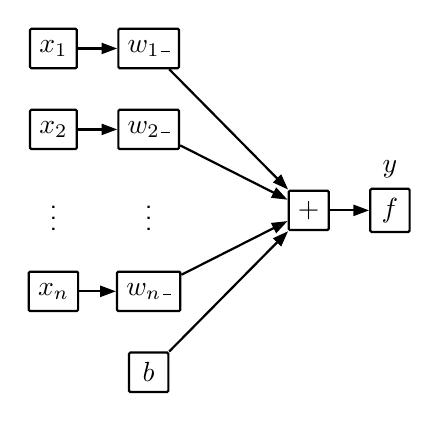
\begin{tikzpicture}
	\tikzstyle{borderless}=[nrect, draw=none]
	\def\inp{\_}
	
	\node[nrect] (x1) {$x_1$};
	\node[nrect] (x2) [below=of x1] {$x_2$};
	\node[borderless] (xdots) [below=of x2] {};
	\node[nrect] (xn) [below=of xdots] {$x_n$};
	\path (x2) -- node[auto=false]{\vdots} (xn);
	
	\node[nrect] (w1) [right=of x1] {$w_1\inp$};
	\node[nrect] (w2) [below=of w1] {$w_2\inp$};
	\node[borderless] (wdots) [below=of w2] {};
	\node[nrect] (wn) [below=of wdots] {$w_n\inp$};
	\path (w2) -- node[auto=false]{\vdots} (wn);	
	\foreach \i in {1,2,n}
	\path (x\i) edge [dedge] (w\i);
	\node[nrect] (b) [below=of wn] {$b$};
	
	\node[nrect] (+) [right=15mm of wdots] {$+$};	
	\foreach \i in {1,2,n}
	\path (w\i) edge [dedge] (+);
	\path (b) edge [dedge] (+);
	
	\node[nrect] (f) [right=of +] {$f$};
	\path (+) edge [dedge] (f);
	\node[above=0 of f] {$y$};
	\end{tikzpicture}
	\caption{Grafički prikaz umjetnog neurona. $w\_$ označava da se u $w$ množi s ulazom čvora.}
	\label{fig:umjetni-neuron}
\end{figure}

Za razliku od modela opisanih u odjeljku~\ref{sec:poopceni-linearni-modeli}, za ovakav i dublje modele opisane u sljedećim odjeljcima ciljna funkcija nije konveksna (ni unimodalna) pa nije garantirano da će postupak učenja pronaći dobru hipotezu. Empirijski rezultati ipak pokazuju da duboke mreže uz neke prilagodbe uspješno uče i generaliziraju. Algoritmi koji se koriste za učenje modela dubokog učenja temelje se na gradijentnom spustu. Oni su opisani u odjeljku~\ref{sec:du-ucenje}.


\section{Duboke unaprijedne mreže}

Može se pokazati da model mreže s jednim skrivenim slojem opisan jednadžbom~\eqref{eq:jednonslojna-nm}, ako je dimenzija skrivenog sloja dovoljno velika, može s proizvoljno malom greškom aproksimirati svaku neprekinutu funkciju kojoj je domena konveksni podskup od $\R$. O tome govori teorem o univerzalnoj aproksimaciji \citep{Cybenko:ASSF:1989,Leshno:1993:MFFNWNPA}. Aktivacijska funkcija mora biti nelinearna jer kompozicija linearnih funkcija je linearna funkcija. Teorem o univerzalnoj aproksimaciji ne govori o tome hoće li takav model generalizirati. Dodavanjem jedinica u skriveni sloj povećava se kapacitet modela.

Obična neuronska mreža može imati više skrivenih slojeva, što se može prikazati kao na slici~\ref{fig:neuronska-mreza} ili apstraktnije, kao na slici~\ref{fig:racunski-graf}. Povećavanjem broja skrivenih slojeva svaka jedinica u nekom sloju može koristiti izlaze svih jedinica prethodnog sloja kao značajke, što mreži omogućuje da, u odnosu na mrežu s $1$ skrivenim slojem, s manje jedinica modelira funkcije u kojima postoje uzorci koji se ponavljaju i imaju hijerarhijsku strukturu \citep{Goodfellow:2016:DL}. Posebne vrste dubokih modela koji uz to iskorištavaju još neke pretpostavke su zato jako uspješne u zadacima u vezi slika, zvuka, teksta i drugih signala. Niži slojevi služe višim slojevima kao značajke transformiranjem kojih se dobivaju značajke više razine.

\begin{figure}
\centering
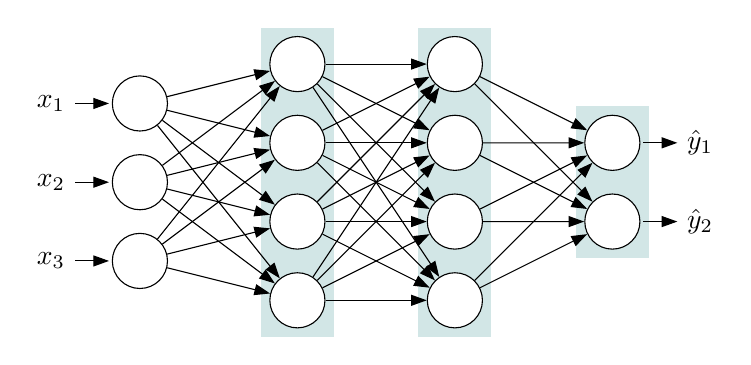
\begin{tikzpicture}[->,draw=black!100, node distance=\layersep]
	\definecolor{lcolor}{RGB}{210,230,230}
	\definecolor{inputcolor}{RGB}{0,0,0}	
	\pgfdeclarelayer{background}
	\pgfsetlayers{background,main}
	\tikzstyle{every pin edge}=[<-,shorten <=1pt]
	\tikzstyle{neuron}=[circle, minimum size=7mm, draw=black!100, fill=white]
	\tikzstyle{layer}=[rectangle, fill=lcolor, minimum size=17pt, inner sep=3pt, outer sep=0pt]
	\def\layersep{2cm}
	\def\inputsize{3}
	\def\hiddensize{4}
	
	% Draw the input layer nodes
	\foreach \name/\y in {1,...,\inputsize} % the same as \foreach \name / \y in {1/1,2/2,3/3,4/4}
	\node[neuron, pin=left:$x_\y$] (I-\name) at (0,-\y) {};
	% Draw the hidden layer nodes
	\foreach \layer in {1,2}
	 \foreach \name/\y in {1,...,\hiddensize}
	  \path[yshift=0.5cm] node[neuron] (H-\layer-\name) at (\layer*\layersep,-\y cm) {};
	% Draw the output layer nodes
	\foreach \name/\y in {1,2}
	 \path[yshift=-0.5cm] node[neuron,pin={[pin edge={->}]right:$\hat{y}_\y$}] (O-\name) at (3*\layersep,-\y cm) {};
	% Connect every node in the input layer with every node in the hidden layer.
	\foreach \source in {1,...,\inputsize}
	 \foreach \dest in {1,...,\hiddensize}
	  \path (I-\source) edge (H-1-\dest);
	% Connect every node in the input layer with every node in the hidden layer.
	\foreach \source in {1,...,\hiddensize}
	 \foreach \dest in {1,...,\hiddensize}
	  \path (H-1-\source) edge (H-2-\dest);
	% Connect every node in the hidden layer with the output layer
	\foreach \source in {1,...,\hiddensize}
	 \foreach \dest in {1,2}
	  \path (H-2-\source) edge (O-\dest);
	
	\begin{pgfonlayer}{background}
	 \node[layer, fit=(H-1-1) (H-1-\hiddensize)] {};
	 \node[layer, fit=(H-2-1) (H-2-\hiddensize)] {};
	 \node[layer, fit=(O-1) (O-2)] {}; 
	\end{pgfonlayer}
\end{tikzpicture}
\caption{Prikaz primjera troslojne mreže. Svakom bridu odgovara jedna težina (pomaci nisu prikazani). Slojevi su označeni plavim četverokutima. Čvorovi koji su unutar četverokuta mreže predstavljaju umjetne neurone. Slika je napravljena prema \url{http://www.texample.net/tikz/examples/neural-network/}.}
\label{fig:neuronska-mreza}
\end{figure}

\begin{figure}
	\centering
	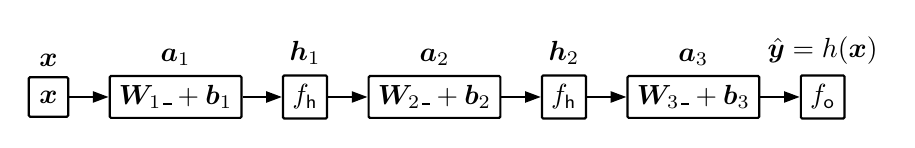
\begin{tikzpicture}
	\def\inp{\_}
	\node[nrect] (x) {$\vec x$};
		\node[above=0 of x] {$\vec x$};
	\node[nrect] (h1a) [right=of x] {$\vec W_1\inp+\vec b_1$};
		\node[above=0 of h1a] {$\vec a_1$};
	\node[nrect] (h1f) [right=of h1a] {$f_\text{h}$};
		\node[above=0 of h1f] {$\vec h_1$};
	\node[nrect] (h2a) [right=of h1f] {$\vec W_2\inp+\vec b_2$};
		\node[above=0 of h2a] {$\vec a_2$};
	\node[nrect] (h2f) [right=of h2a] {$f_\text{h}$};
		\node[above=0 of h2f] {$\vec h_2$};
	\node[nrect] (oa) [right=of h2f] {$\vec W_3\inp+\vec b_3$};
	\node[nrect] (y) [right=of oa] {$f_\text{o}$};
		\node[above=0 of oa] {$\vec a_3$};
	\node[above=0 of y] {$\hat{\vec y}=h(\vec x)$};
	\path (x) edge [dedge] (h1a);	
	\path (h1a) edge [dedge] (h1f);
	\path (h1f) edge [dedge] (h2a);
	\path (h2a) edge [dedge] (h2f);
	\path (h2f) edge [dedge] (oa);
	\path (oa) edge [dedge] (y);
	\end{tikzpicture}
	\caption{Prikaz troslojne mreže kao računskog grafa. Čvorovi predstavljaju funkcije s parametrima, a bridovi podatke (vektore) čije su oznake prikazane uz neke od čvorova iz kojih izlaze. Funkcije su označene oznakom funkcije (aktivacijska funkcija) ili definicijom (afina transformacija). Ulaz sloja označen je s $\_$, a oznake varijabli koje pripadaju čvorovima (ulaz u ulaznom čvoru i parametri u čvorovima afine transformacije) nisu podvučene.}
	\label{fig:racunski-graf}
\end{figure}

Kao prijenosna funkcija skrivenih slojeva često se koristi \emph{zglobnica} (\emph{ReLU}, engl. rectified linear unit) $\ReLU(x)=\max(0, s)$ za koju se empirijski pokazalo da ima prednosti nad funkcijama koju su prije bile češće korištene \citep{Glorot:2011:DSRNN}. Prije su češće bile korištene \emph{logistička funkcija}, $\sigma(s)=\frac{\exp(s)}{1+\exp(s)}$, i \emph{tangens hiperbolni}, $\tanh(x)=\frac{\exp(s)-\exp(-s)}{\exp(s)+\exp(-s)}$. U izlaznom sloju obično se koriste funkcije korištene kod poopćenih linearnih modela (odjeljak~\ref{sec:poopceni-linearni-modeli}) -- identitet za regresiju, logistička funkcija za binarnu klasifikaciju, a \emph{softmaks}, $\softmax(\vec s)=\frac{1}{\cvec 1^\tp\exp(\vec s)}\exp(\vec s)$, koji kao izlaz daje normalizirani vektor koji predstavlja razdiobu, za višeklasnu klasifikaciju. Na slici \ref{fig:prijenosne-funkcije} prikazani su grafovi nekih prijenosnih funkcija.

\begin{figure}
	\centering
	\includegraphics[width=1\linewidth]{transfer-functions}
	\caption[s]{Primjeri prijenosnih funkcija.}
	\label{fig:prijenosne-funkcije}
\end{figure}

Dosad opisivane mreže nazivaju se \emph{unaprijedne mreže} (engl. \textit{feedforward networks}) zato što se pri izračunu informacija propagira od ulaza prema izlazu, bez povratnih veza. Za mrežu kažemo da je duboka ako ime veći broj slojeva. Struktura duboke unaprijedne mreže ne mora se sastojati samo od niza afinih transformacija i nelinearnosti. Općenito, mrežu možemo predstaviti \emph{računskim grafom}, tj. usmjerenim acikličkim grafom kod kojega čvorovi predstavljaju varijable ili računske operacije i njihove izlaze, a bridovi označavaju ovisnosti, tj. koji čvor je ulaz kojeg čvora. Svaki čvor koji nije ulazni predstavlja funkciju koju ostvaruje podgraf koji čine njegovi preci pa ga možemo poistovjetiti s funkcijom čiji su parametri svi ulazni čvorovi iz skupa čvorova predaka. Čvorovi koji nemaju roditelje su varijable koje čine ulazi i parametri. Parametri se mogu dijeliti, tj. mogu biti ulaz većem broju čvorova kao i svi drugi čvorovi. Čvorovi koji nemaju djecu su izlazi računskog grafa. Na slici \ref{fig:umjetni-neuron} i \ref{fig:racunski-graf} su prikazani takvi grafovi s različitim razinama apstrakcije. U njima, radi sažetosti, parametri nemaju zasebne čvorove, nego su označeni unutar čvorova koji o njima ovise.

\section{Učenje} \label{sec:du-ucenje}

Cilj učenja je pronaći parametre $\vec\theta$ koji minimiziraju pogrešku
\begin{align}
E(\vec\theta;\set D) = \frac{1}{\envert{\set D}}\sum_{(\vec x_i,\vec y_i)\in\set D} L(\vec y_i,h(\vec x_i;\vec\theta)) + \lambda R_\text{R}(\vec\theta)
\end{align}
i postići dobru generalizaciju. Duboki modeli se obično uče algoritmima koji se temelje na gradijentnom spustu. Gradijent pogreške s obzirom na parametre je
\begin{align} \label{eq:gs-ucenje}
\nabla_{\vec\theta}E(\vec\theta;\set D) = \frac{1}{\envert{\set D}}\sum_{(\vec x_i,\vec y_i)\in\set D} \nabla_{\vec\theta}L(\vec y_i,h(\vec x_i;\vec\theta)) + \lambda \nabla_{\vec\theta}R_\text{R}(\vec\theta) \text{.}
\end{align}
Kod dubokih mreža, tj. usmjerenih acikličkih računskih grafova, gradijent se računa \emph{algoritmom propagacije pogreške unatrag} \citep{Rumelhart:1986:LIREP} koji se temelji na \emph{pravilu deriviranja kompozicije funkcija} i \emph{dinamičkom programiranju}. 

U ovom odjeljku su kratko opisane ideje korištene za efikasno računanje gradijenta i optimizacijski postupci koji se koriste za pronalaženje dobrih parametara kod dubokih mreža.

\subsection{Algoritam propagacije pogreške unatrag}

Na ovaj pododjeljak ima utjecaj \cite{Olah:2015:CCGB}.

Gradijent gubitka nije potrebno analitički računati za svaki parametar posebno. Primjenom pravila deriviranja složene funkcije, derivacija vrijednosti nekog čvora $b$ s obzirom na čvor vrijednost nekog čvora $a\in\pred(b)$ jednaka je zbroju umnožaka parcijalnih derivacija \textit{dijete-roditelj} čvorova po svakom putu između $a$ i $b$. Pri tome je put definiran kao niz takav da sljedeći (usmjereni) brid počinje u čvoru u kojem je prethodni završio. Svakom bridu $(p,c)$ odgovara derivacija $\pd{c}{p}$. Derivacije između susjednih čvorova ne moraju se računati za svaki put posebno. Već izračunate derivacije se mogu ponovo koristiti. Isto vrijedi ako su vrijednosti čvorova vektori (ako su višedimenzionalni nizovi, možemo ih svesti na vektore) i ako računamo Jakobijeve matrice. Dalje će se za Jakobijeve matrice isto koristiti riječ \textit{derivacija}.

Algoritam propagacije pogreške unatrag se tako naziva zato što se izračun gradijenta širi od izlaznog čvora (ili čvora koji predstavlja gubitak ili funkciju pogreške) prema njegovim roditeljima, pa prema roditeljima roditelja itd. uz primjenu pravila deriviranja kompozicije funkcija. Pri tome se ne moraju računati gradijenti s obzirom na čvorove koji ne ovise o varijablama za koje se računa gradijent.

Neka je $L$ vrijednost čvora gubitka, a $\vec\theta$ neki parametar. Želimo izračunati gradijent $\nabla_{\vec\theta_i}L=\pd{L}{\vec\theta}^\tp$. Derivacija gubitka s obzirom na čvoru $u$ se može rekurzivno izraziti: 
\begin{align} \label{eq:gradijent-rekurzivno}
\pd{L}{u} = \sum_{c\in\ch(u)} \pd{L}{c}\pd{c}{u}	\text{,}
\end{align}
gdje su $c$ djeca čvora $u$. Ako $\pd{L}{c}$ nije izračunat za trenutni ulaz, izračuna se, a inače se koristi prethodno izračunata vrijednost. Ista jednadžba vrijedi za čvorove parametara.

Neka je zadatak nadzirano učenje, $\set D=\cbr{\vec x_i, \vec y_i}_i$ skup podataka za učenje, a $L_i=L(\vec y_i, h(\vec x_i,\vec \theta))$ gubitak para $(\vec x_i, \vec y_i)$. Neka je pogreška npr. $E=\sum_i L_i + R_\text{R}(\vec\theta)$. Onda
\begin{align}
\pd{E}{\vec\theta} 
= \sum_{i} \pd{L_i}{\vec\theta} + \pd{R_\text{R}}{\vec\theta}\del{\vec\theta} \text{,}
\end{align}
gdje se izrazi na desnoj strani računaju rekurzivno uz pamćenje izračunatih gradijenata (ili unaprijed izračunate gradijente koji odgovaraju bridovima u podgrafu koji se sastoji od čvorova potomaka) prema jednadžbi~\ref{eq:gradijent-rekurzivno}.

\subsection{Gradijenti nekih osnovnih operacija}

U tablici~\ref{tab:derivacije} prikazane su parcijalne derivacije (Jakobijeve matrice) nekih operacija s obzirom na njihove ulaze. Korištenjem pravila deriviranja kompozicije funkcija mogu se izračunati derivacije složenijih funkcija. Radi efikasnosti se izračunavanje vrijednosti u računskom grafu i algoritam propagacije pogreške unatrag provodi paralelno za više ulaza odjednom. Izvodi gradijenata nekih operacija uz višestruke ulaze mogu vidjeti npr. ovdje: \url{http://www.zemris.fer.hr/~ssegvic/du/lab0.shtml}. 

\begin{table}
	\centering
	\begin{tabular}{|P{0.5\textwidth}|P{0.4\textwidth}|}
		\hline
		\bfseries Operacija & \bfseries Derivacije \\
		\hline
		$\vec y = \vec W \vec x + \vec b$
		& $\pd{\vec y}{\vec x} = \vec W$ \newline
		$\pd{\vec y}{\del{\vec W_\ind{i,:}}^\tp} = \vec x^\tp$ \newline
		$\pd{\vec y}{\vec b} = \cvec I$
		\\\hline
		$\vec y = \vec a \concat \vec b$
		& $\pd{\vec y}{\vec a} = \diag\del{\cvec 1_{\dim(\vec a)}\concat\cvec 0_{\dim(\vec b)}}$ \newline
		$\pd{\vec y}{\vec b} = \diag\del{\cvec 0_{\dim(\vec a)}\concat\cvec 1_{\dim(\vec b)}}$
		\\\hline
		$\vec y = \ReLU(\vec x)$
		& $\pd{\vec y_\ind{i}}{\vec x_\ind{j}} = 
		 \enbbracket{i=j} \enbbracket{\vec x_\ind{j}>0} $
		\\\hline
		$\vec y = \sigma(\vec x)$
		& $\pd{\vec y}{\vec x} =
		 \diag\del{\vec y\odot\del{\cvec1-\vec y}}$
		\\\hline
		$\vec y = \tanh(\vec x)$
		& $\pd{\vec y}{\vec x} =	
		 \diag\del{1 - \vec y\odot\vec y}$
		\\\hline
		$\vec y = \softmax(\vec x)$
		& $\pd{\vec y_\ind{i}}{\vec x_\ind{j}} = \vec y_\ind{j}\del{\enbbracket{i=j}-\vec y_\ind{j}}$
		\\\hline
		$y = -t\ln\sigma(x)-(1-t)\ln\del{1-\sigma(x)}$
		& $\pd{y}{x} = \sigma(x)-t$
		\\\hline
		$y = -\ln\softmax(\vec x)_\ind{t}$
		& $\pd{y}{\vec x} = \del{\softmax(\vec x)-\cvec e_t}^\tp$
		\\\hline
	\end{tabular}
	\caption{Parcijalne derivacije (Jakobijeve matrice) nekih operacija po njihovim ulazima. Zadnja sva retke predstavljaju gubitak unakrsne entropije (negativni logaritam izglednosti) za binarnu i višeklasnu klasifikaciju, gdje je $t$ indeks ciljne klase. $\cvec e_t$ označava jednojedinični vektor s elementima $\cvec {e_t}_\ind{i}=\enbbracket{i=t}$.}
	\label{tab:derivacije}
\end{table}


\subsection{Stohastička optimizacija} \label{subsec:dukn-stoh-optimizacija}

U pododjeljku~\ref{subsec:gradijenti-spust} opisan je gradijentni spust i neki izvedeni algoritmi koji koriste neke dodatne heuristike. U ovom pododjeljku opisana je primjena tih algoritama u dubokom učenju. Kod učenja dubokih modela se obično koristi puno podataka i iteracija optimizacije se provodi procjenjivanjem gradijenta funkcije pogreške na temelju manjeg dijela skupa za učenje.

Kod \emph{stohastičkog gradijentnog spusta} se u nekoj iteraciji gradijentnog spusta umjesto gradijenta pogreške koristi gradijent procjene pogreške na temelju nekog podskupa skupa za učenje ili samo jednog primjera. Takav algoritam naziva se \emph{stohastički gradijentni spust}. Moguće je podskupove u svakoj iteraciji ponovo slučajno izvlačiti iz cijelog skupa za učenje $\set D$, ali obično se iteracije podijele na \emph{epohe} od kojih se svaka sastoji od $B$ iteracija, u svakoj epohi se skup za učenje slučajno podijeli na $B$ nepreklapajućih podskupova $\set D_i$ jednake veličine, od kojih se svaki koristi u jednoj iteraciji unutar epohe. Skupove $\set D_i$ nazivamo \emph{mini-grupe}. U iteraciji $i$ u nekoj epohi koristi se procjena gradijenta
\begin{align} \label{eq:sgs-ucenje}
\nabla_{\vec\theta}E(\vec\theta;\set D_i) = \frac{1}{\envert{D_i}}\sum_{(\vec x_i,\vec y_i)\in\set D_i} \nabla_{\vec\theta}L(\vec y_i,h(\vec x_i;\vec\theta)) + \lambda \nabla_{\vec\theta}R_\text{R}(\vec\theta) \text{.}
\end{align}
i iteracija (prema jednadžbi~\eqref{eq:gs}) ima oblik
\begin{align} \label{eq:sgs}
\vec \theta_i = \vec \theta_{i-1} - \eta\nabla_{\vec\theta}E(\vec\theta;\set D_{i})\text{,}
\end{align}
gdje je $e$ broj epohe, a $i+1$ broj trenutne iteracije unutar epohe.

Prema \citet{Goodfellow:2016:DL}, na odabir veličine mini-grupe utječu:
\begin{enumerate}
	\item Kvaliteta procjene gradijenta. Veće minigrupe daju točniju procjenu gradijenta.
	\item Računska efikasnost. Premale mini-grupe ne iskorištavaju potpuno mogućnost paralelizacije izračuna, a prevlike grupe ne stanu u memoriju.
	\item Optimizacija s manjim mini-grupama ima učinak regularizacije \citep{Wilson:2003:GIBTGDL}, ali zahtijeva manju stopu učenja i sporije konvergira.
\end{enumerate}

Kako bi optimizacijski algoritam konvergirao, treba se smanjivati stopa učenja ovisno o iteraciji (epohi). Prema \cite{Goodfellow:2016:DL}, dovoljan uvjet za konvergenciju gradijentnog spusta je
\begin{align}
\sum_{k=1}^\infty \eta_k=\infty \wedge \sum_{k=1}^\infty \eta_k^2<\infty \text{,}
\end{align}
gdje je $k$ broj iteracije od početka učenja.

Kako bi se ublažio šum procjene gradijenta i ubrzalo učenje, obično se upotrebljava inercija, kao što je opisano u pododjeljku~\ref{subsec:gradijenti-spust}. Empirijski se pokazuje da stohastički gradijentni spust s momentom postiže dobru generalizaciju. U pododjeljku~\ref{subsec:gradijenti-spust} su opisana i dva algoritma koja koriste pokretne prosjeke momenata gradijenta i prilagođeni su stohastičkom učenju s mini-grupama. RMSProp skalira gradijent po elementima korištenjem pokretnog prosjeka kvadrata gradijenta tako da norma elemenata pomaka ne ovisi jako o prosječnoj normi gradijenta u zadnjim iteracijama. Adam koristi inerciju i obavlja skaliranje slično kao RMSProp.


\subsection{Inicijalizacija parametara}

Kod učenja dubokih modela jako je bitna inicijalizacija parametara. Sve težine mreže (ili dijela nje), npr. kao na slici~\ref{fig:neuronska-mreza}, se ne smiju se inicijalizirati konstantnom vrijednošću. Zamjenom dvaju jedinica istog sloja, npr. kao na slici~\ref{fig:neuronska-mreza}, dobiva se ista mreža i gradijent je jednak za sve težine unutar istog sloja, osim za zadnji sloj. To se rješava inicijalizacijom težina nasumičnim vrijednostima. Ako su inicijalizirane težine manje, sporije će se \textit{razbijati} simetrija, a ni prevelike težine nisu dobre. Ako se koriste prijenosne funkcije sa zasićenjem problem mogu biti težine s prevelikom apsolutnim vrijednostima jer mogu uzrokovati zasićenje i tako onemogućavati učenje. Taj problem rješava zglobnica, ali množenjem velikih težina kroz više slojeva daje sve veće izlaze, što kod linearnih slojeva daje prevelik gradijent, što se vidi u tablici~\ref{tab:derivacije}.

Heuristike korištene za inicijalizaciju težina se temelje na aproksimiranju mreže nizom matričnih množenja i postizanju da varijance gradijenata (i izlaza) budu otprilike konstantne kroz mrežu \citep{Goodfellow:2016:DL}. Otprilike konstantna varijanca gradijenta može se ostvariti inicijalizacijom iu Guassove ili unifomne razdiobe s varijancom $\frac{1}{n}$, gdje je $n$ broj ulaza. \citet{Glorot:2010:UDTDFNN} kao kompromis između jednake varijance gradijenta i jednake varijance izlaza slojeva predlažu varijancu $\frac{1}{n+m}$, gdje je $m$ broj izlaza \citep{Goodfellow:2016:DL}.

Pomaci se obično inicijaliziraju na neku konstantu.

\subsection{Problem nekonveksnosti funkcije pogreške}

\citet{Goodfellow:2016:DL} navode sljedeće probleme koji se javljaju kod nekonveksne optimizacije:
\begin{enumerate}
	\item \emph{Loše kondicioniranje Hesseove matrice}. Loše kondicioniranje Hesseove matrice može biti razlog da i s jako malim korakom učenje funkcija pogreške raste u smjeru gradijenta zato što kvadratni član u Taylorovom rezvoju u jednadžbi~\eqref{eq:grad-delta-approx}  bude pozitivan i prevlada linearni član.
	\item \emph{Lokalni minimumi}. I ako se zanemare ekvivalentni lokalni minimumi koji postoje zbog simetričnosti zamjenjivosti položaja neurona u istom sloju i drugih simetričnosti u neurnoskim mrežama, funkcija pogreške ima velik broj lokalnih minimuma. Empirijski se pokazuje da loši lokalni minimumi nisu problem i da nije potrebno pronaći globalni minimum kako bi se dobili dobri rezultati.
	\item \emph{Ostale stacionarne točke}. Kod visokodimenzionalnih optimizacijskih problema lokalni minimumi i maksimumi su obično rijetki zato što bi onda sve vlastite vrijednosti Hesseove matrice morale biti istog predznaka. Zato su češće sedlaste točke kod kojih se predznak barem jedne vlastite vrijednosti razlikuje od predznaka ostalih. Empirijski se pokazuje da sedlaste točke kod dubokih mreža nisu velik problem za optimizacijske postupke prvog reda koje ne privlače sedlaste točke. I ako se parametri nalaze točno u sedlastoj točki tako da je gradijent $\cvec 0$, stohastički gradijentni spust može imati drugačije gradijente.
	\item \emph{Litice i eksplodirajući gradijenti}. Kod nekih modela javlja se problem velikih vrijednosti gradijenta u nekim točkama. To se može riješiti ograničavanjem norme gradijenta.
\end{enumerate}


\section{Regularizacija i poboljšavanje učenja}

U ovom pododjeljku opisani su neki od češćih postupaka koji se koriste za poboljšavanje učenja, tj. postizanja bolje generalizacije i bržeg učenja. Dijelovi ovog pododjeljka temelje se na \citet{Goodfellow:2016:DL}, gdje se može naći opširniji i dublji pregled.

\subsection{Kažnjavanje norme težina}

Najjednostavniji način regularizacije je kažnjavanje norme težina. Regularizacijski dio funkcije pogreške $R_\text{R}$ se najčešće definira kao kvadrat $L^2$ norme, tj. koristi se \emph{$L^2$ regularizacija} koja odgovara apriornoj pretpostavci Gaussove razdiobe težina s dijagonalnom kovarijacijskom matricom i očekivanjem $\vec 0$. Može se koristiti i \emph{$L^1$ regularizacija} koja potiče rijetkost težina, tj. postavlja minimum funkcije pogreške u ovisnosti o nekim težinama točno u $0$. To je detaljnije objašnjeno npr. u \citet{Goodfellow:2016:DL}. $L^1$ regularizacija odgovara Laplaceovoj apriornoj razdiobi.  Općenito, gubitak $L^p$ regularizacije ima oblik:
\begin{align}
	R_\text{R}(\vec\theta) 
	= \frac{\lambda}{p}\enVert{\vec\theta}_p^p 
	= \frac{\lambda}{p}\sum_i \envert{\vec\theta_\ind{i}}^p \text{,}
\end{align}
gdje $\lambda$ određuje jačinu regularizacije, tj. koncentraciju apriorne razdiobe. Gustoći apriorne razdiobe odgovara
\begin{align}
\p(\vec\theta) &= \frac{1}{Z}\exp(-R_\text{R}(\vec\theta)) \\
&= \frac{1}{Z}\prod_i\exp\del{-\frac{\lambda}{p}\envert{\vec\theta_\ind{i}}^p} \text{,}
\end{align}
gdje je $Z$ normalizacijska konstanta. Gradijent regularizacijskog gubitka s obzirom na $\vec\theta_\ind{i}$ je $\lambda\sgn(\vec\theta_\ind{i})\envert{\vec\theta_\ind{i}}^{p-1}$. Posebno, to je  $\lambda\vec\theta_\ind{i}$ za $p=2$ i  $\lambda\sgn(\vec\theta_\ind{i})$ za $p=1$.

\subsection{Rano zaustavljanje učenja}

Regularizacijski učinak koji se može usporediti s $L^p$ regularizacijom ima \emph{rano zaustavljanje} učenja zato što ograničava koliko se parametri mogu udaljiti od početne vrijednosti. Ako se model predugo uči, može se dogoditi da se težine modela s velikim kapacitetom previše prilagode skupu za učenje i zato dođe do loše generalizacije.

\subsection{Generiranje podataka}

Postupci koji značajno mogu utjecati na generalizaciju su postupci \emph{proširivanja skupa podataka}, što znači da se tijekom učenja obično provode jednostavne slučajne transformacije nad primjerima prije nego što se daju kao ulaz modelu. Primjeri transformacija koje se mogu koristiti u računalnom vidu, ovisno o zadatku, su reflektiranje, translacija i rotacija. Generiranje podataka kod zadataka koji imaju veze sa zvukom isto može biti korisno \cite{Goodfellow:2016:DL}.

Dodavanje šuma ulazu isto može biti korisno \citep{Goodfellow:2016:DL}. To odgovara pretpostavci da primjeri koji su slični u ulaznom prostoru trebaju biti slični i u izlaznim prostoru.

Pokazalo se da je moguće pronaći ulazne primjere koji su u ljudskoj percepciji slični prirodnim primjerima, ali i modeli koji ostvaruju rezultate usporedive s rezultatima ljudi daju krive predikcije \citep{Szegedy:2013:IPNN,Goodfellow:2014:EHAE}. Takvi ulazni primjeri nazivaju se \emph{neprijateljski primjeri}. Oni se mogu dobiti i pomoću jednog koraka gradijentnog spusta pomicanjem ulaznog primjera u smjeru povećavanja gubitka. Jedan od uspješnijih načina postizanja otpornosti na neprijateljske primjere je proširivanje skupa za učenje neprijateljskim primjerima \citep{Madry:2017:TDLMRAA}.

\subsection{Isključivanje neurona - dropout}

\emph{Dropout} \citep{Hinton:2012:INNPCAFD,Srivastava:2014:DASWPNNO} je postupak regularizacije koji unosi šum u izlaze skrivenih slojeva tijekom učenja. Obično se ostvaruje tako da se tijekom učenja za svaki primjer svaka jedinica mreže isključi s vjerojatnošću $p$, koja je hiperparametar. Tijekom testiranja, tj. zaključivanja, sve se jedinice skaliraju s $1-p$, tj. očekivanjem skaliranja koje je tijekom učenja $0$ s vjerojatnošću $p$, a $1$ s vjerojatnošću $1-p$. Dropout se obično primjenjuje nakon afine transformacije (ne nakon aktivacije).

Učenje s \textit{dropoutom} se može interpretirati kao učenje eksponencijalnog broja modela koji dijele parametre, a zaključivanje kao aproksimacija usrednjavanja modela ili aproksimacija bayesovskog zaključivanja. Vremenski zahtjevniji, ali ispravniji postupak usrednjavanj modela bio bi uzorkovanje \citep{Srivastava:2014:DASWPNNO}, tj. \textit{Monte Carlo} aproksimacija izlaza. \citet{Gal:2016:DBARMUDL} su dali bayesovku interpretaciju takvog usrednjavanja. 

Umjesto Bernoullijeve razdiobe, skaliranje ili izlazi jedinica mogu imati npr. Gaussovu razdiobu ili neku drugu.

\subsection{Normalizacija po grupama}

Normalizacija po grupama (engl. \textit{batch normalization}) \citep{Ioffe:2015:BNADNTRUCS} je postupak koji ublažava probleme pri učenji i omogućuje učenja jako dubokih modela. Prema \citet{Goodfellow:2016:DL}, problem kod učenja jako dubokih modela je što se se sastoje od kompozicije velikog broja funkcija, zbog čega je velika međuzavisnost između parametara različitih slojeva, a u koraku gradijentnog spusta parametri svih funkcija ažuriraju se istovremeno. Gradijenti spust pretpostavlja da je utjecaj svakog parametra lokalno nezavisan, tj. svaka se funkcija (sloj afine transformacije) prilagođava ostatku mreže kakav je u trenutnom koraku, tj. očekuje da se prethodni slojevi neće promijeniti.

U \cite{Goodfellow:2016:DL} je to objašnjeno na jednostavnom primjeru $\hat y=xw_1w_2,\bidot,w_j$, gdje su elementi gradijenta $g_i=\nabla_{\vec w_i}\hat y=x\prod_{j\neq i}w_j$. Novi izlaz nakon koraka gradijentnog spusta je $x\prod_i(w_i-\epsilon g_i)$ gdje članovi uz više potencije $\epsilon$ mogu imati utjecaj koji raste eksponencijalno s dubinom $l$.

Sloj normalizacije po grupama se dodaje nakon sloje linearne transformacije (prije prijenosne funkcije). On kod učenja obavlja ovakvu operaciju:
\begin{align} \label{eq:bn}
	\vec Y = \del{\vec X-m(\vec X)}\oslash s(\vec X) \text{,}
\end{align}
gdje je $\vec X=\sbr{\vec x_i}_{i=1\bidot N}^\tp\in\R^{N\times n}$ matrica kojoj su reci vektori značajki pojedinih primjera, $\vec Y=\sbr{\vec y_i}_{i=1\bidot N}^\tp\in\R^{N\times n}$ matrica kojoj su reci značajke normalizirane ulazne značajki, $m(\vec X)\coloneqq\frac{1}{N}\sum_i\vec X_\ind{i,:}\in\R^{1\times n}$ srednja vrijednost vektora značajki, $s(\vec X)\coloneqq\del{\frac{1}{N}\sum_i\del{\vec X_\ind{i,:}-m(\vec X)}^{\odot 2}}^{\odot\frac{1}{2}}\in\R^{1\times n}$ standardna devijacija vektora značajki po elementima. Oduzimanje u jednadžbi~\eqref{eq:bn} je definirano tako da se od svakog retka $\vec X$ oduzima $m(\vec X)$. Takvo značenje ima i dijeljenje. Izlaz sloja normalizacije po grupama tijekom učenja je invarijantan na skaliranje i pomak ulaza $\vec X$.

Statistike grupe, tj. srednje vrijednosti i standardne devijacije od grupe za koju se provodi zaključivanje, se koriste samo kod učenja. Inače se koriste statistike skupa za učenje koje se mogu procijenjivati pokretnim prosjekom tijekom učenja. Računski graf normalizacije po grupama kod učenja i kod ispitivanja je prikazan na slici \ref{fig:bn-graf}.

\begin{figure}
	\centering
	\begin{subfigure}[t]{0.48\textwidth}
		\centering
		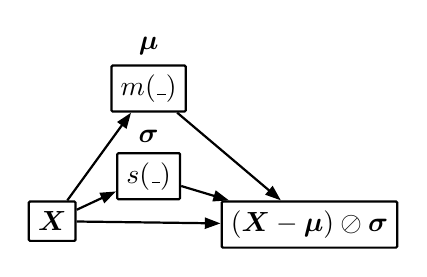
\begin{tikzpicture}
		\tikzstyle{borderless}=[nrect, draw=none]
		\def\inp{\_}
		\node[nrect] (x) [] {$\vec X$};
		\node[nrect] (s) [above right=0mm and 5mm of x] {$s(\inp)$};
		\node[nrect] (m) [above=of s] {$m(\inp)$};
		\node[above=0 of m] {$\vec\mu$};		
		\node[above=0 of s] {$\vec\sigma$};
		\node[nrect] (bn) [below right=0 and 5mm of s] {$(\vec X-\vec\mu)\oslash\vec\sigma$};
		
		\path (x) edge [dedge] (m);
		\path (x) edge [dedge] (s);
		
		\path (s) edge [dedge] (bn);
		\path (m) edge [dedge] (bn);
		\path (x) edge [dedge] (bn);
		\end{tikzpicture}
		\caption{Graf normalizacije po grupama kod učenja.}
		\label{subfig:bn-ucenje}
	\end{subfigure}
	~
	\begin{subfigure}[t]{0.48\textwidth}
		\centering
		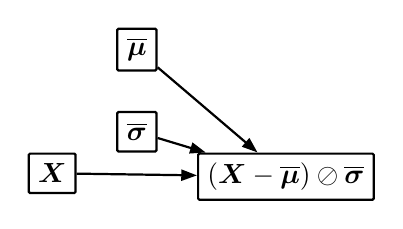
\begin{tikzpicture}
		\tikzstyle{borderless}=[nrect, draw=none]
		\def\inp{\_}
		\node[nrect] (x) [] {$\vec X$};
		\node[nrect] (s) [above right=0mm and 5mm of x] {$\overline{\vec\sigma}$};
		\node[nrect] (m) [above=of s] {$\overline{\vec\mu}$};

		\node[nrect] (bn) [below right=0 and 5mm of s] {$(\vec X-\overline{\vec\mu})\oslash\overline{\vec\sigma}$};
		
		\path (s) edge [dedge] (bn);
		\path (m) edge [dedge] (bn);
		\path (x) edge [dedge] (bn);
		\end{tikzpicture}
		\caption{Graf normalizacije po grupama kod ispitivanja.}
		\label{subfig:bn-ispitivanje}
	\end{subfigure}
	\caption{Grafovi normalizacije po grupama kod učenja i kod ispitivanja. $m$ i $s$ su funkcije koje računaju srednju vrijednost i standardnu devijaciju grupe. $\overline{\vec\mu}$ je srednja vrijednost, a $\overline{\vec\sigma}$ standardna devijacija ulaza kod skupa za učenje.}
	\label{fig:bn-graf}
\end{figure}

Kako se ne bi izgubila ekspresivnost, nakon sloja normalizacije po grupama obično se dodaje pomak $\vec\beta\in\R^{1\times n}$ i skaliranje $\vec\gamma\in\R^{1\times n}$ svake značajke. $\vec\beta$ i $\vec\gamma$ su parametri koji se uče. Kod ispitivanja je normalizacija po grupama uz skaliranje i pomak samo drugačija parametrizacija koja je uz prethodni sloj linearne transformacije s težinama $\vec W$ može svesti na sloj afine transformacije s težinama $\vec W\oslash\vec\sigma^\tp\odot\vec\gamma^\tp$ i pomacima $-\vec\mu\oslash\sigma\odot\vec\gamma+\vec\beta$.

Kod konvolucijskih mreža se normalizacija po grupama ne provodi samo po dimenziji grupe, nego i po dimenzijama konvolucije, po kojima treba vrijediti translacijska ekvivarijantnost. Npr. ako je ulazni niz dimenzija $N\times H\times W\times C$, gdje je $N$ veličina grupe, $H$ visina slike, $W$ širina slike, a $C$ broj značajki, tj. broj filtara zadnje konvolucije, vektor srednjih vrijednosti i vektor srandardnih odstupanja je dimenzije $C$, tj. $1\times 1\times 1\times C$.

%\subsection{Dijeljenja parametara, pomoćni gubici i višezadaćno učenje}
%višezadaćno učenje, pomoćni gubici, dijeljenje parametara


\section{Konvolucijske mreže}

\emph{Konvolucijske mreže} su mreže koje, prema definiciji u \citet{Goodfellow:2016:DL}, na barem jednom mjestu, umjesto općenite linearne transformacije, koriste \emph{konvoluciju}. Konvolucijske mreže koriste pretpostavku \emph{translacijske ekvivarijantnosti} po nekim dimenzijama ulaza i posebno se uspješno primjenjuju na zadacima u vezi slika. Pojedini elementi izlaza \emph{konvolucijskog sloja} računaju se množenjem manjeg \emph{filtra} s elementima ulaza koje on prekriva na svakom položaju ulaza. Element i izlaza ovise o malom broju elemenata ulaza oko odgovarajućih položaja, tj. \emph{povezanost} je \emph{lokalna}. To omogućuje da se broj parametara konvolucijskog sloja značajno smanji u odnosu na \emph{potpuno-povezani sloj}, tj. sloj linearne transformacije. Pojedine težine uče se na različitim dijelovima ulaza i to sve omogućuje veću efikasnost i bolju generalizaciju.

\subsection{Konvolucija}

Konvolucija funkcija iz $\Z\to\R$ definirana je ovim izrazom:
\begin{align}
(f*g)(t) \coloneqq \sum_\tau f(\tau)g(t-\tau) \text{.}
\end{align}
Jednako tako, definirana je konvolucija funkcija iz $\Z^n\to\R$:
\begin{align}
(f*g)(\vec t) \coloneqq \sum_{\vec\tau} f(\vec\tau)g(\vec t-\vec\tau) \text{.}
\end{align}
Na isti način, s integralom umjesto zbroja, definirana je i konvolucija funkcija s kontinuiranom domenom. Neka od svojstava konvolucije su:
\begin{enumerate}
	\item Komutativnost: $f*g=g*f$.
	\item Distributivnost zbrajanja. Vrijedi $(f+g)*h=f*h+g*h$.	
	\item Translacijska ekvivarijantnost. Ako $f'(t) \coloneqq f(t+d)$, onda $(f'*g)(t)=(f*g)(t+d)$.
	\item Konvolucija u vremenskoj domeni odgovara umnošku u Fourierovoj domeni, tj. $\const F[f*g]=\const F[f]\const F[g]$, gdje $\const F$ označava odgovarajuću Fourierovu transformaciju \citep{Jeren:2015:SISC55}.
\end{enumerate}

Konvolucija se može poopćiti na funkcije s kodomenom koja može općeniti vektorski prostor, tj. funkcije iz $\Z^m\to\R^n$. Jedan način je ovaj, gdje se po svakoj komponenti paralelno obavlja konvolucija:
\begin{align}
(f*_\text{p}g)(\vec t) \coloneqq 
\sum_{\vec\tau} f(\vec\tau)\odot g(\vec t-\vec\tau) \text{.}
\end{align}
Drugi način je ovaj, gdje se izlazni vektori funkcija skalarno množe:
\begin{align} \label{eq:konvolucija-s}
(f*_\text{s}g)(\vec t) \coloneqq 
\sum_{\vec\tau} \braket{f(\vec\tau)}{g(\vec t-\vec\tau)} \text{.}
\end{align}
U ovom slučaju, kodomena funkcije $f*_\text{s}g$ je $\R$. Isti izraz vrijedi i ako je kodomena funkcija $f$ i $g$ neki skup $n$-dimenzionalnih nizova, tj. $\R^{d_1\times\dots\times d_n}$, gdje su $d_i$ pojedine dimenzije niza. Zato se za skalarni produkt ovdje koristi oznaka skalarnog produkta.

\subsection{Konvolucijski sloj}

Jednom umjetnom neuronu kod konvolucijskih mreža, ako se zanemari pomak, obično odgovara operacija u jednadžbi~\eqref{eq:konvolucija-s}, samo što funkcijama $f$ i $g$ odgovaraju konačni $(m+1)$-dimenzionalni (ili $m$-dimenzionalni ako $n=1$) nizovi pa treba prilagoditi definiciju konvolucije na nizove. Jednoj funkciji odgovara ulazni niz, a drugoj \emph{konvolucijska jezgra} (\emph{filtar}) koja je obično manja i neovisna o veličini ulaza. Izlaz konvolucije je onda $m$-dimenzionalni niz kojem su dimenzije obično iste kao privih $m$ dimenzija ulaznog niza, ovisno o prilagodbi definicije konvolucije na nizove. Ovakvu konvoluciju ćemo nazivati \emph{$m$-dimenzionalna konvolucija}. Ovdje se neće razmatrati $m$-dimenzionalna konvolucija $(m+n)$-dimenzionalnih nizova kod kojih $n>1$, tj. $\vec A_\ind{i_1,\bidot,i_m,:}$ su vektori ako je $\vec A$ $(m+1)$-dimenzionalan.

Slojevi koji obavljaju konvoluciju nazivaju se \emph{konvolucijski slojevi}. Izlaz jedne jedinice (dobiven jednim filtrom) u konvolucijskom sloju naziva se \emph{mapa značajki}. Izlaz konvolucijskog sloja sastoji se od više mapa značajki i čini $(m+1)$-dimenzionalni izlaz kojem je zadnja dimenzija jednaka broju mapa značajki. $m$-dimenzionalnu konvoluciju s $k$ jezgri nazivat ćemo \emph{$k$-struka $m$-dimenzionalna konvolucija}.

Osnovni način definiranja $m$-dimenzionalne konvolucije (unakrsne korelacije ako ne reflektiramo jezgru) $(m+1)$-dimenzionalnog ulaza $\vec X$ s $(m+1)$-dimenzionalnom jezgrom $\vec W$, što daje $m$-dimenzionalni niz $\vec X*_\text{s}\vec W$, može se ovako izraziti:
\begin{align} \label{eq:konvolucija-sv}
(\vec X*_\text{s}^\text{v}\vec W)_\ind{\vec t} \coloneqq 
\braket{\vec X_\ind{\vec t:\vec t+ \vec d_{\vec W}+\cvec 1,:}}{\vec W} \text{,}
\end{align}
gdje je $\vec d_{\vec W} = \dim(\vec W)_\ind{1:m}$ vektor dimenzija jezgre po kojima se obavlja konvolucija. Skalarni produkt na desnoj je definiran ako $\forall i \in \cbr{1\bidot m}\ {\vec t}_\ind{i} \in \cbr{1,\bidot,{\vec d_{\vec X}}_\ind{i}-{\vec d_{\vec W}}_\ind{i}-1}$, gdje je $\vec d_{\vec X}=\dim(\vec X)_\ind{1:m}$ vektor dimenzija ulaza. Izlaz takve operacije je dimenzija $\del{{\vec d_{\vec X}}_\ind{i}-{\vec d_{\vec W}}_\ind{i}-\cvec 1}$.
Kod obrade slike obično želimo da izlaz konvolucije bude jednakih dimenzija kao ulaz. To se može ostvariti dopunjavanjem ulaza nulama po rubu dimenzija po kojima treba obavljati konvoluciju tako da sredina jezgre, za koju pretpostavljamo da ima neparne dimenzije, može doći do ruba originalnog ulaza. Neka $\mathrm{pad}\del{\vec X, \tfrac{1}{2}\del{\vec d_{\vec W}-\cvec 1}}$ označava takvu operaciju dopunjavanja. Definiramo novu operaciju:
\begin{align} \label{eq:konvolucija-ss}
\vec X *_\text{s}^\text{s} \vec W \coloneqq 
\mathrm{pad}\del{\vec X, \tfrac{1}{2}\del{\vec d_{\vec W}-\cvec 1}} *_\text{s}^\text{v} \vec W \text{.}
\end{align}
U gornjem indeksu operatora "v" dolazi od riječi \textit{valid} zato što se filtar pomiče samo unutar granica ulaza, a "s" od riječi \textit{same} zato što je izlaz istih dimenzija kao ulaz (osim zadnje). Na slici~\ref{fig:konvolucija-dopunjavanje} ilustrirani su najčešći načina dopunjavanja na primjeru jednostruke dvodimenzionalne konvolucije dvodimenzionalnih nizova. Na slici~\ref{fig:konvolucija-grafovi} prikazana je jednostruka jednodimenzionalna konvolucija (unakrsna korelacija) dvodimenzionalnih nizova s dopunjavanjem kao u jednadžbi~\eqref{eq:konvolucija-ss}. 

\begin{figure}
	\centering
	\begin{subfigure}[t]{0.31\textwidth}
		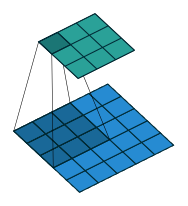
\includegraphics[width=1\textwidth]{konv/no_padding_no_strides_00_i3}
		\caption{Bez dopunjavanja.}
		\label{subfig:konv-nopad}
	\end{subfigure}
	~
	\begin{subfigure}[t]{0.31\textwidth}
		\centering
		\includegraphics[width=1\textwidth]{konv/same_padding_no_strides_00}
		\caption{Dopunjavanje takvo da izlaz ima iste dimenzije kao ulaz.}
		\label{subfig:konv-samepad}
	\end{subfigure}
	~
	\begin{subfigure}[t]{0.31\textwidth}
		\centering
		\includegraphics[width=1\textwidth]{konv/full_padding_no_strides_00}
		\caption{Potpuno dopunjavanje.}
		\label{subfig:konv-fullpad}
	\end{subfigure}
	\caption{Ilustracija dopunjavanja kod dvodimenzionalne konvolucije. Slika~\ref{subfig:konv-samepad} i slika~\ref{subfig:konv-fullpad} su preuzete, a slika~\ref{subfig:konv-nopad} je napravljena na temelju slika iz \citet{Dumoulin:2016:GCADL}.}
	\label{fig:konvolucija-dopunjavanje}
\end{figure}

\begin{figure}
\centering
\begin{subfigure}[t]{0.48\textwidth}
	\centering
	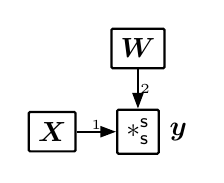
\begin{tikzpicture}
	\tikzstyle{borderless}=[nrect, draw=none]
	\def\inp{\_}
	\node[nrect] (x) [] {$\vec X$};	
	\node[nrect] (y) [right=of x] {$*_\text{s}^\text{s}$};
	\node[nrect] (w) [above=of y] {$\vec W$};
	\node[right=0 of y] {$\vec y$};
	\path (w) edge [dedge] node[right=-1mm]  {\tiny $2$} (y);
	\path (x) edge [dedge] node[above=-1mm]  {\tiny $1$} (y);
	\end{tikzpicture}
	\caption{Apstraktni prikaz konvolucije.}
	\label{subfig:konv-aps}
\end{subfigure}
~
\begin{subfigure}[t]{0.48\textwidth}
	\centering
	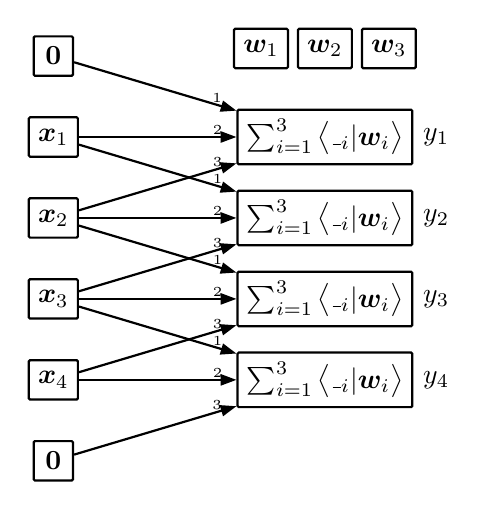
\begin{tikzpicture}
	\tikzstyle{borderless}=[nrect, draw=none]
	\def\inp{\_}
	\def\n{4}
	
	\node[nrect] (x0) {$\cvec 0$};
	\foreach \i in {1,2,...,\n}
	  \pgfmathtruncatemacro\result{\i-1}
	  \node[nrect] (x\i) [below=5mm of x\result] {$\vec x_\i$};
	\pgfmathtruncatemacro\result{\n+1}
	\node[nrect] (x\result) [below=5mm of x\n] {$\cvec 0$};
	
	\foreach \i in {1,2,...,\n} {
	  \node[nrect] (y\i) [right=20mm of x\i] {$\sum_{i=1}^3 \braket{\inp_i}{\vec w_i}$};
	  \node[right=0 of y\i] {$y_\i$};
	}
	\foreach \i in {1,2,...,\n}
	  \foreach \j in {1,2,3}
	    \pgfmathtruncatemacro\result{\i+\j-2}
	    \path (x\result) edge [dedge] node[above=-1mm,pos=0.88] {\tiny $\j$} (y\i);
	\node[nrect] (w2) [above=of y1] {$\vec w_2$};
	\node[nrect] (w1) [left=1mm of w2] {$\vec w_1$};
	\node[nrect] (w3) [right=1mm of w2] {$\vec w_3$};
	\end{tikzpicture}
	\caption{Detaljniji prikaz konvolucije.}
\label{subfig:konv-det}
\end{subfigure}
	\caption{Grafički prikaz jednodimenzionalne konvolucije s dopunjavanjem. Na slici~\subref{subfig:konv-det} detaljnije su prikazani dvodimenzionalni nizovi $\vec X\in\R^{4\times n}$ i $\vec W\in\R^{3\times n}$ iz slike~\subref{subfig:konv-aps} rastavljeni na vektore, dopunjavanje i konvolucija na razini vektora $\vec x_i=\vec X_\ind{i,:}$ i $\vec w_i=\vec W_\ind{i,:}$. Rezultat konvolucije je $\vec y=\sbr{y_1,\bidot,y_4}\in\R^4$. $\__i$ označava $i$-ti ulaz čvora u smjeru obrnutom od kazaljke na satu od desne strane.}
	\label{fig:konvolucija-grafovi}
\end{figure}


\subsubsection{Izlazni korak konvolucije i dilatacija jezgre}

Kod konvolucijski mreža još se koriste neke izmjene konvolucije kako bi se postigla veća računalna efikasnost. Jedna je korištenje \emph{izlaznog koraka} (ili \emph{korak}). Izlazni korak veći od $1$ da jezgra po toj dimenziji preskače neke položaje. Na taj način se postiže da dimenzije izlaza budu manje za otprilike za faktor veličine izlaznog koraka. Konvolucija s Izlazniim korakom $2$ po svim dimenzijama konvolucije ilustrirana ja na slici~\ref{fig:konvolucija-izl-korak}. 

\begin{figure}
	\centering
	\includegraphics[width=0.24\textwidth]{konv/no_padding_strides_00}
	\includegraphics[width=0.24\textwidth]{konv/no_padding_strides_01}
	\includegraphics[width=0.24\textwidth]{konv/no_padding_strides_02}
	\includegraphics[width=0.24\textwidth]{konv/no_padding_strides_03}
	\caption{Ilustracija konvolucije s korakom $2$. Slike su preuzete iz \citet{Dumoulin:2016:GCADL}.}
	\label{fig:konvolucija-izl-korak}
\end{figure}

Kako bi se povećalo \emph{receptivno polje} jedinice konvolucijskog sloja bez povećavanja dimenzija jezgre, koristi se konvolucija s \emph{dilatacijom} (ili \emph{dilacijom}), tj. \emph{širenje jezgre}. Na slici~\ref{fig:konvolucija-dilatacija} ilustrirana konvolucija s dilacijom $1$. Takva konvolucija je ekvivalentan konvoluciji kod koje se koristi veća jezgra kod koje se svaki drugi redak ili stupac sastoji od nula.

\begin{figure}
	\centering
	\includegraphics[width=0.24\textwidth]{konv/dilation_00}
	\includegraphics[width=0.24\textwidth]{konv/dilation_01}
	\includegraphics[width=0.24\textwidth]{konv/dilation_02}
	\includegraphics[width=0.24\textwidth]{konv/dilation_03}
	\caption{Ilustracija konvolucije s dilacijom $1$. Slike su preuzete iz \citet{Dumoulin:2016:GCADL}.}
	\label{fig:konvolucija-dilatacija}
\end{figure}

\subsubsection{Konvolucija kao matrično množenje}

Konvolucija je linearna operacija. Na slici~\ref{fig:konvolucija-konk} je konvolucija sa slike~\ref{fig:konvolucija-grafovi} prikazana malo drugačije. Jezgra je pretvorena u vektor, a ulaz je pretvoren u vektore koji se skalarno množe s vektorom koji predstavlja jezgru. Možemo ulaz $\vec X$ pretvoriti u matricu $\vec X_\text{M}\in\R^{4\times 3n}$, a jezgru $\vec W$ u vektor $w\in\R^{3n}$ tako da njihov matrični umnožak daje izlaz konvolucije:
\begin{align}
\underbrace{
\begin{bmatrix}
\cvec 0_{1\times n} & \vec x_1^\tp & \vec x_2^\tp \\
       \vec x_1^\tp & \vec x_2^\tp & \vec x_3^\tp \\
       \vec x_2^\tp & \vec x_3^\tp & \vec x_4^\tp \\
       \vec x_3^\tp & \vec x_4^\tp & \cvec 0_{1\times n}         
\end{bmatrix}
}_{\vec X_{\text{M}}}
\underbrace{
\begin{bmatrix}
\vec w_1 \\
\vec w_2 \\
\vec w_3     
\end{bmatrix}
}_{\vecfunc(\vec W)}
=
\underbrace{
\begin{bmatrix}
y_1 \\ y_2 \\ y_3 \\y_4     
\end{bmatrix}
}_{\vec y}
\text{.}
\end{align}

Konvolucijski sloj obično ima više jezgri $\vec W_i$. Sada se lako vidi da vrijedi $\pd{\vec y}{\vecfunc(\vec W)}=\vec X_\text{M}$. To možemo poopćiti na $k$-struku konvoluciju:
\begin{align}
\vec X_\text{M}
\begin{bmatrix}
\vecfunc(\vec W_1) & \vecfunc(\vec W_2) & \cdots & \vecfunc(\vec W_k)
\end{bmatrix}
= 
\begin{bmatrix}
\vec y_1 & \vec y_2 & \cdots & \vec y_k \\
\end{bmatrix}
\text{.}
\end{align}

\begin{figure}
	\centering
	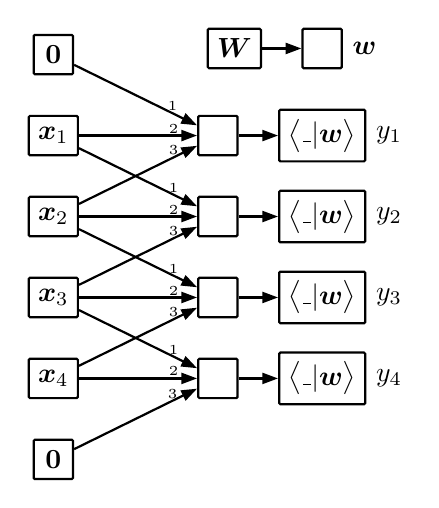
\begin{tikzpicture}
	\tikzstyle{borderless}=[nrect, draw=none]
	\def\inp{\_}
	\def\n{4}
	
	\node[nrect] (x0) {$\cvec 0$};
	\foreach \i in {1,2,...,\n}
		\pgfmathtruncatemacro\result{\i-1}
		\node[nrect] (x\i) [below=5mm of x\result] {$\vec x_\i$};
	\pgfmathtruncatemacro\result{\n+1}
	\node[nrect] (x\result) [below=5mm of x\n] {$\cvec 0$};
	
	%\node[nrect] (X) [below left=0 and 15mm of x3] {$\vec X$};
	
	\foreach \i in {1,2,...,\n} {
		%\path (X) edge [dedge] (x\i);		
		\node[nrect] (xx\i) [right=15mm of x\i] {$\concat$};
		\node[nrect] (y\i) [right=of xx\i] {$\braket{\inp}{\vec w}$};
		\node[right=0 of y\i] {$y_\i$};
	}
	\foreach \i in {1,2,...,\n} {
		\foreach \j in {1,2,3}
			\pgfmathtruncatemacro\result{\i+\j-2}
			\path (x\result) edge [dedge] node[above=-1mm,pos=0.8] {\tiny $\j$} (xx\i);
		\path (xx\i) edge [dedge] (y\i);
	}
	\node[nrect] (w) [above=of y1] {$\vecfunc$};
	\node[right=0 of w] {$\vec w$};
	\node[nrect] (W) [left=of w] {$\vec W$};
	\path (W) edge [dedge] (w);
	\end{tikzpicture}
	\caption{Alternativni prikaz konvolucije ekivalentan onom na slici~\ref{fig:konvolucija-grafovi}. $\concat$ ovdje označava združivanje vektora $\vec x_i\in\R^n$ u vektor iz $\R^{3n}$, $\vecfunc$ funkciju koja $\vec W\in\R^{3\times n}$ preslikava u $\vec w\in\R^{3n}$.}
	\label{fig:konvolucija-konk}
\end{figure}

To se može poopćiti i na višedimenzionalnu konvoluciju \citep{Sharan:2014:EPDL}. Onda su reci matrice $\vec X_\text{M}$ vektori $\vecfunc\del{\mathrm{pad}\del{\vec X, \tfrac{1}{2}\del{\vec d_{\vec W}-\cvec 1}}_\ind{\vec t:\vec t+\vec {d^{\vec W}}_\ind{1:m}+\cvec 1,:}}$ redom po $\vec t$, uz oznake iz jednadžbe~\eqref{eq:konvolucija-sv}, tj. reci su vektori koji sadrže elemente ulaza koje \textit{pokriva} jezgra za svaki položaj. Jezgra je opet vektor, a kao izlaz se dobije vektor koji treba preoblikovati tako da mu prvih $m$ dimenzija bude jednako prvih $m$ dimenzija ulaza.

Drugi način pretvaranja konvolucije u matrično množenje je ovakav: 
\begin{align}
\underbrace{
\begin{bmatrix}
\vec w_2^\tp & \vec w_3^\tp & \cvec 0_{1\times n} & \cvec 0_{1\times n} \\
\vec w_1^\tp & \vec w_2^\tp & \vec w_3^\tp & \cvec 0_{1\times n} \\
\cvec 0_{1\times n} & \vec w_1^\tp & \vec w_2^\tp & \vec w_3^\tp \\
\cvec 0_{1\times n} & \cvec 0_{1\times n} & \vec w_1^\tp & \vec w_2^\tp 
\end{bmatrix}
}_{\vec W_\text{M}}
\underbrace{
	\begin{bmatrix}
	\vec x_1 \\ \vec x_2 \\ \vec x_3 \\ \vec x_4 
	\end{bmatrix}
}_{\vecfunc(\vec X)}
= 
\underbrace{
	\begin{bmatrix}
	y_1 \\ y_2 \\ y_3 \\y_4     
	\end{bmatrix}
}_{\vec y}
\text{.}
\end{align}
Ovdje se vidi da $\pd{\vec y}{\vecfunc(\vec X)}=\vec W_\text{M}$. Gradijent gubitka $L$ po ulazu je $\del{\pd{L}{\vec y}\pd{\vec y}{\vecfunc(\vec X)}}^\tp = \vec W_\text{M}^\tp\nabla_{\vec y}L$. To isto odgovara jednoj vrsti konvolucije koja se naziva \emph{transponirana konvolucija} \citep{Segvic:2018:DUUUKS}.

\subsection{Slojevi sažimanja}

U konvolucijskim mrežama se, uglavnom radi smanjivanja dimenzija, mogu koristiti \emph{slojevi sažimanja}. Operacije sažimanja, slično konvolucijskim slojevima, primjenjuju neku funkciju pomicanjem okna po dimenzijama konvolucije, obično s korakom većim od 1. Za razliku od konvolucijskih slojeva, oni obično djeluju na svakoj mapi značajki posebno i izlazi sažimanja su invarijantni na zamjenu elemenata unutar okna. To svojstvo se naziva \emph{lokalna invarijantnost}. Najčešće se kao funkcija koja preslikava skup elementa okna u izlaz koristi $\max$ ili prosjek. Veličina okna je često jednaka veličini koraka tako da se susjedna okna ne preklapaju. Na slici~\ref{fig:sazimanje-primjeri}.

\begin{figure}
	\centering
	\begin{subfigure}[t]{0.48\textwidth}
		\includegraphics[width=1\textwidth]{konv/numerical_average_pooling_00}
		\caption{Sažimanje prosječnom vrijednošću s oknom dimenzija $3\times 3$ i korakom $1$.}
		\label{subfig:avg-pool}
	\end{subfigure}
	~
	\begin{subfigure}[t]{0.48\textwidth}
		\centering
		\includegraphics[width=1\textwidth]{konv/numerical_max_pooling_00}
		\caption{Sažimanje maksimalnom vrijednošću s oknom dimenzija $3\times 3$ i korakom $1$.}
		\label{subfig:max-pool-31}
	\end{subfigure}
	\vskip\baselineskip
		\begin{subfigure}[t]{0.48\textwidth}
		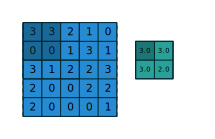
\includegraphics[width=1\textwidth]{konv/numerical_max_pooling_00_i22}
		\caption{Sažimanje maksimalnom vrijednošću s oknom dimenzija $2\times 2$ i korakom 2.}
		\label{subfig:max-pool-22}
	\end{subfigure}
	~
	\begin{subfigure}[t]{0.48\textwidth}
		\centering
		\includegraphics[width=1\textwidth]{konv/numerical_max_pooling_00_ig}
		\caption{Globalno sažimanje maksimalnom vrijednošću.}
		\label{subfig:max-pool-g}
	\end{subfigure}
	\caption{Ilustracije primjera dvodimenzionalnog različitih sažimanja. Slike su preuzete iz \citet{Dumoulin:2016:GCADL} i prilagođene.}
	\label{fig:sazimanje-primjeri}
\end{figure}


\chapter{Procjenjivanje nesigurnosti}


\section{Aleatorna i epistemička nesigurnost}

Kod bayesovskih modela nesigurnost zaključivanja izražava se razdiobom po vrijednostima varijable čija vrijednost se procjenjuje, a može se izraziti i entropijom ili varijancom kada je prikladno.

Postoje različiti izvori nesigurnosti \citep{Kennedy:2002:BCCM}, ali nesigurnost općenito možemo podijeliti na dvije vrste: \emph{aleatornu nesigurnost} i \emph{epistemičku nesigurnost} \citep{Kiureghian:2009:AEDM}. Riječ \textit{aleatorna} izvedena je vjerojatno od latinske riječi \textit{aleator} \citep{Gal:2016:UDL} koja znači \textit{kockar}, a riječ \textit{epistemička} izvedena je od grčke riječi \textit{epist\={e}m\={e}} koja znači \textit{znanje}. Aleatorna nesigurnost je nesigurnost koju model ne može smanjiti neovisno o znanju i količini dostupnih podataka. Ona dolazi od nedeterminizma samog procesa koji generira podatke, nedostupnosti dijela informacija ili ograničenja modela. Epistemička nesigurnost je nesigurnost u strukturu i parametre modela \citep{Gal:2016:UDL}. Ona dolazi od neznanja i može se smanjiti uz više podataka.

Granica između aleatorne i epistemičke nesigurnosti ovisi o modelu. Nešto što je kod jednostavnijeg modela aleatorna nesigurnost, kod složenijeg modela može biti epistemičkog karaktera. Ako su neke pojave po prirodi nasumične ili se ne mogu ili ne žele modelu dati informacije koje bi ih mogle objasniti, nesigurnost zaključivanja u vezi tih pojava će, neovisno o ograničenosti modela, biti aleatorna.

\section{Homoskedastička i heteroskedastička aleatorna nesigurnost}

Aleatorna nesigurnost može biti homoskedastička i heteroskedastička.

TODO: homoskedastička, heteroskedastička nesigurnost

TODO: model uncertainty, predictive uncertainty Gal-thesis 1.2

\the\fontdimen5\font\newline % em
\the\fontdimen6\font\newline % ex
small {\small \the\fontdimen6\font\newline} % ex}
footnotesize {\footnotesize \the\fontdimen6\font\newline} % ex}
\the\textwidth
		
\begin{figure}
	\centering
	\includegraphics[width=1.0\textwidth]{homoscedastic-heteroscedastic-noises}
	\caption{Homoskedastički (lijevo) i heteroskedastički (desno) Gaussov šum.  Crta prikazuje očekivanje $f(x)$, svjetloplava površina standardnu devijaciju šuma $s(x)$, a točke slučajne uzorke. Točke su generirane prema $(\rvar y\mid x) \sim \mathcal{N}(f(x),s(x)^2)$. Na lijevoj slici je $s(x)=1$.}
	\label{fig:homoscedastic-heteroscedastic-noises}
\end{figure}
		
		

\chapter{Nesigurnost kod dubokih mreža}


\section{Bayesovske neuronske mreže}


\chapter{Eksperimentalni rezultati}


\section{Programska izvedba}


\section{Skupovi podataka}



\chapter{Zaključak}

Zaključak.

\bibliography{literatura}
\bibliographystyle{fer}

\begin{sazetak}
Sažetak na hrvatskom jeziku.

\kljucnerijeci{Ključne riječi, odvojene zarezima.}
\end{sazetak}

% TODO: Navedite naslov na engleskom jeziku.
\engtitle{Title}
\begin{abstract}
Abstract.

\keywords{Keywords.}
\end{abstract}

\end{document}
